\documentclass[a4paper,10pt]{report}

\usepackage[in]{fullpage}
\usepackage{parskip}
\usepackage{hyperref}
\usepackage{tikz}
\usepackage{amsmath}
\usepackage[backend=bibtex,style=numeric-comp,sorting=nyt,sortcites=true,maxnames=4]{biblatex}
\usepackage[section]{placeins}
\usepackage[color,cntglobally]{circus}
\usepackage{fixltx2e}
\usepackage{comment}

\usetikzlibrary{calc}

\setcounter{secnumdepth}{4}

\title{A Framework for Verifying Safety-Critical Java Virtual Machines}
\author{James Baxter}
\date{}

\bibliography{literature} 

\setcounter{secnumdepth}{4}

\CountDefsfalse

\newif\ifFullModel
\FullModelfalse
\newcommand{\ifnFullModel}{\ifFullModel\else}

\newcommand{\directsubclass}{\prec_\mathrm{d}}
\newcommand{\directsubclassid}{\prec_\mathrm{D}}
\newcommand{\subclassid}{\preceq}

%TC:group zed 0 displaymath
%TC:group axdef 0 displaymath
%TC:group schema 1 displaymath
%TC:group circus 0 displaymath
%TC:group circusaction 0 displaymath
%TC:macroword \Circus 1
%TC:group theorem 1 displaymath
%TC:group zproof 0 displaymath 

\begin{document}
\maketitle

\begin{abstract}
  In recent years Java has been increasingly considered as a language
  for safety-critical embedded systems.
  However, some features of Java are unsuitable for such systems and
  this has resulted in the creation of Safety-Critical Java (SCJ).
  The different scheduling and memory management model of SCJ means
  that a specialised virtual machine is required to run SCJ programs.
  Given the safety-critical nature of the applications, it must be
  ensured that the virtual machine is correct, but so far no SCJ
  virtual machine has been formally verified.
  In this dissertation, we propose a framework for verification of SCJ
  virtual machines.
  We consider the differences between SCJ and standard Java, and
  discuss some of the existing virtual machines for SCJ.
  Seeing that many SCJ virtual machines precompile to native code, we
  then survey some of the literature on compiler correctness.
  Finally, we present some preliminary results identifying the
  requirements of the services of an SCJ virtual machine and
  constructing a formal model of those requirements.
\end{abstract}

\tableofcontents


\chapter{Introduction}

This chapter begins by explaining the motivation for the work
described in this dissertation.
Afterwards, the objectives of the work, which come from the
motivation, are described and, finally, the structure of the remainder
of this dissertation is described.

\section{Motivation}

Since its release in 1995, the Java programming
language~\cite{gosling2013} has increased in popularity and is now in
use on many platforms.
This popularity means that Java has been used in a wide variety of
areas including desktop applications, on the internet in the form of
Java applets, on smartcards~\cite{chen2000} and on mobile
devices~\cite{oracle2014}.
Several languages derived from Java have also been created, including
Scala~\cite{lausanne2015} and Ceylon~\cite{redhat2015}, as well as
older variants of Java such as MultiJava~\cite{clifton2006} and
Pizza~\cite{odersky1997}, which have in turn contributed to the
development of Java.
Scala adds functional programming features to Java, some of which have
been incorporated into Java 8.
Ceylon extends Java's type system with features such as union types,
allowing some common Java errors to be checked at compile time through
the type system.

One use of Java that is of particular interest is in embedded systems.
While early versions of Java were developed for programming embedded
systems, particularly TV set-top boxes, the technology was not well
received.
It was only in the growing sector of the internet that Java initially
found a market~\cite{horstmann2002}.
However, it was soon realised that the portability, modularity, safety
and security benefits of Java could be of great use in embedded
systems~\cite{mulchandani1998}.
This required the creation of specialised Java virtual machines as the
standard JVM is too large for most embedded systems.
Much research has gone into making smaller and smaller virtual
machines to widen the range of devices that Java can be used
on~\cite{caska2011,thomm2010}.

Many embedded systems are also real-time systems, and features of Java
such as the garbage collector and the concurrency model make it
unsuitable for real-time systems, for which strict guarantees about
timing properties must be made.
To address this issue the Real-Time Specification for Java
(RTSJ)~\cite{gosling2000} was created.
The RTSJ extends Java with a scoped memory model and a more
predictable scheduling system.

While the RTSJ addresses real-time requirements of embedded systems,
many embedded systems are also safety-critical.
For these conformance to certain standards, such as \mbox{DO-178C} and
ISO~26262, is required.
To support the development of safety-critical programs that meet these
requirements in Java, the Safety-Critical Java (SCJ)
specification~\cite{locke2013} has been created.
SCJ is a subset of the RTSJ that removes the features that cannot be
easily statically reasoned about, which means that features such as
the garbage-collected heap and dynamic class loading are absent from
SCJ.
This facilitates the creation of SCJ programs that fulfil formal
specifications; indeed work has already been done on developing
correct SCJ programs from formal specifications~\cite{cavalcanti2011,
  cavalcanti2013}.

On the other hand, even if it can be shown that SCJ programs are
correct, it must still be ensured those programs are executed
correctly.
In the case of Java-like languages, this generally means ensuring the
Java compiler and Java Virtual Machine (JVM) are correct.

Work has been done on modelling virtual machines for Java, and on the
formal correctness of compilers targeting those virtual machines.
Some of the most complete work in that area was by St\"{a}rk, Schmid
and B\"{o}rger~\cite{stark2001}, who present a model of the full Java
language and virtual machine, along with a formally verified compiler,
although for an older version of Java than is current.
Other work has also been done on modelling the JVM and Java
compilation using refinement techniques~\cite{duran2010}.
Additionally there has been work considering machine checked models of
Java virtual machines and compilers~\cite{lochbihler2012, nipkow2000,
  strecker2002}.
Work has also been done on the semantics of Java bytecode and
verification of standard JVMs~\cite{bertelsen2000, jones1998}.

However, SCJ has a number of differences from standard Java.
Firstly, as already indicated the SCJ memory model is rather different
to the standard Java memory model, abandoning the garbage collector in
favour of a scoped memory model.
Garbage collection is less predictable and often quite complex, and so
difficult to reason about and unsuitable for some of the strictest
certifiability requirements of safety-critical systems.
By contrast, the scoped memory model provides greater predictability
on when memory is freed.
Similarly, the SCJ approach to scheduling differs from that of
standard Java, using a preemptive priority scheduling approach rather
than the unpredictable scheduling of standard Java threads.
These differences of SCJ from standard Java mean that the standard JVM
is not suitable for running SCJ programs.
A specialised virtual machine is required.

In the case of virtual machines for embedded systems, the priorities
are usually size and speed, which generally results in machines that
are hard to verify.
Moreover, virtual machines that rely on interpreting bytecode are
unsuitable for real-time embedded systems as they are likely to be
slower.
An alternative method to run a Java program is to compile it to native
code and some authors have suggested doing so either
directly~\cite{schultz2003} or via C~\cite{varma2004}.
There are several virtual machines that take this approach including
Fiji VM~\cite{pizlo2009}, Icecap HVM~\cite{sondergaard2012} and
OVM~\cite{armbruster2007}.
This allows correct running of an otherwise correct SCJ program to be
viewed as a compiler verification problem.

There has been much research into compiler correctness.
Much of the work follows a commuting diagram approach, in which the
compilation is shown to be consistent with transformation between the
semantics of the source and target languages\cite{morris1973,
  thatcher1979}.
This approach is apparent in much of the early work such as that of
McCarthy and Painter~\cite{mccarthy1967}, as well as in more recent
work such as the CompCert project~\cite{leroy2009a, leroy2009b}.
There has also been work that follows this approach and employs
automated theorem provers~\cite{klein2006, milner1972, nipkow2000}.
They provide additional certainty that the proof is correct and can
also provide code generation facilities to allow creation of a working
compiler.

An alternative is the algebraic approach to compiler
verification~\cite{hoare1991, sampaio1993}, based on modelling
compilation using refinement calculi~\cite{back1981, morgan1990,
  morris1987}.
This approach appears to be less commonly used but has been applied to
Java~\cite{duran2005, duran2010} and hardware description
languages~\cite{perna2010, perna2011}.
This approach is also quite amenable to automation as it relies on
refinement laws that can be applied by a term rewriting system.

There is a clear need for formal verification of SCJ virtual machines
due to the safety-critical nature of the systems involved and the fact
that safety standards such as DO-178C require it at the highest safety
levels.
However, there appears to be little work done in that area and, as far
as we know, no SCJ virtual machine has been formally verified.

% explain that there is a gap with no verification for SCJ compilers
% for embedded systems

\section{Objectives}

Our objective is to develop an approach to verification of an SCJ
virtual machine that allows the production and verification of correct
SCJ virtual machines.
Although the actual creation and verification of such machines is
outside the scope of our work, we provide the following resources for
developers and verifiers:
\begin{itemize}
\item a specification of the requirements of an SCJ virtual machine,
\item a formal model of the virtual machine specification,
\item a compilation strategy from Java bytecode to native C code,
\item proofs for validation of the formal model and verification of
  the compilation strategy, and
\item a mechanisation of the model and proofs.
\end{itemize}

We follow the design of existing SCJ virtual machines to ensure that
our work is of practical relevance to the SCJ community.
We particularly focus on the icecap HVM~\cite{sondergaard2012}, as
that is the only publicly-available SCJ virtual machine that is
up-to-date with the SCJ specification.
Where there are ambiguities or concerns regarding the description of
the virtual machine in the SCJ standard, we take the icecap
implementation as a reference to define the requirements and formal
model for an SCJ virtual machine.
In addition, the native C code generated by our formal compilation
strategy is very close
% TODO: check this near the end of the work when we know what is
% achieved
to that actually produced by icecap.
%This is an assurance of the practical relevance of our results.

Our results can be used to aid the development and verification of an
SCJ virtual machine in several different ways.
The informal specification provides a reference for the requirements
of an SCJ virtual machine


\subsection{SCJ Virtual Machine Specification}

The first component required is a specification of the requirements
for an SCJ virtual machine.
This specification will shape the rest of the work and there is at
present no clear specification of what is required of an SCJ virtual
machine or how it differs from a standard Java virtual machine.
The specification of requirements needs to consider the requirements
imposed, both explicitly and implicitly, on virtual machines by the
SCJ specification~\cite{locke2013} as that provides the authoritative
source for information on SCJ.
It is also helpful to consider the approach taken by some existing SCJ
virtual machines on points where the SCJ specification is unclear.
The virtual machine must also meet the standard Java Virtual Machine
specification~\cite{lindholm2014} on points such as how to interpret
Java bytecode instructions.
There is much existing work on the semantics of Java bytecode that can
be used in our work~\cite{bertelsen2000, jones1998, stark2001}.

\subsection{Compilation Strategy}

As many existing virtual machines for SCJ precompile programs to
native code in order to allow faster execution on embedded systems, it
seems wise to include that in our approach.
We will focus on compilation of Java bytecode to C as that is the
approach adopted by several existing virtual machines for embedded
systems, including Fiji VM~\cite{pizlo2009} and icecap
HVM~\cite{sondergaard2012}, and C is already widely used for embedded
systems software.

There are two main approaches to the specification and verification of
compilers: the commuting diagram approach and the algebraic approach.
The commuting diagram approach involves specifying the compiler as a
function from the source language to the target language and showing
that it is consistent with transformation between the semantics of the
source and target languages~\cite{morris1973, thatcher1979}.
This approach has been used in much of the work on compiler
correctness, including some of the earliest work~\cite{mccarthy1967}
and recent work such as that of the CompCert project~\cite{leroy2009a,
  leroy2009b}.

The algebraic approach involves defining the source and target
languages in the same specification space, and using proved
specialised rewrite rules to characterise compilation as model
transformation in the extended language.
This approach was first proposed in the early nineties by
Hoare~\cite{hoare1991} and further developed by
Sampaio~\cite{hoare1993, sampaio1993}.
The algebraic approach does not seem to be as popular as the commuting
diagram approach, but it does have the advantage that the
specification of the compilation strategy is correct by construction
as the rewrite rules that comprise it have all been proved.

\subsection{Formal Model and Proofs}

In order to ensure that the specification is precise and to facilitate
proofs of its correctness, it must have a model written in some formal
specification language.
We will focus on using the \Circus{} specification
language~\cite{oliveira2009}, as it has been used in some of the
previous work on formalising SCJ~\cite{cavalcanti2011,
  cavalcanti2013}.
It is important that the correctness of the formal models and
compilation strategy can be shown via mathematical proof, which
requires the specification language to have a well-defined semantics.
\Circus{} has such a semantics, defined using the model of Unifying
Theories of Programming (UTP)~\cite{hoare1998}.

\subsection{Mechanisation}

To prevent mistakes in the proofs, it is helpful to mechanise the
formal model and proofs.
There are various systems that can be used for this, but we will focus
on the proof assistant Isabelle~\cite{nipkow2002, nipkow2014}.
It has existing mechanisations of \Circus{}~\cite{feliachi2012} and
the UTP~\cite{foster2015}, and has been used in previous work
verifying compilers for Java-like languages~\cite{klein2006,
  strecker2002, lochbihler2010}, making it well placed for our work.

\subsection{Summary}

In conclusion, our objective is an approach verification of SCJVMs
consisting of mechanised formal models together with proofs of
properties about them.
These formal models will cover both the services that must be provided
by a running SCJVM and a compilation strategy for translating Java
bytecode to native code.
With our results, SCJVM developers will be able to create provably
correct ahead-of-time compiling SCJVM implementations and check the
correctness of those implementations.

\section{Document Structure}

Having given a brief overview of the area of study and identified the
problem we wish to consider, the remainder of this dissertation
proceeds as follows.

In Chapter~\ref{literature-review-chapter} we examine the literature
on safety-critical virtual machines and compilers for Java-like
languages.
This includes a discussion of why a safety-critical variant of Java is
necessary and how it differs from standard Java.
We also explain why a specialised virtual machine is necessary for
SCJ.
This is followed by a survey of the existing virtual machines for
Safety-Critical Java and the techniques used in verifying compilers.

In Chapter~\ref{scjvm-services-chapter} we present an identification of the
requirements of SCJ virtual machine services, with a formal model of
those requirements in the \Circus{} specification language.
This is followed by a model of the an SCJ virtual machine core
execution environment in Chapter~\ref{cee-chapter}.

Finally, we conclude in Chapter~\ref{conclusions-chapter} by
summarising our contributions and mentioning the wider context of this
research.

\chapter{Compilers and Virtual Machines for Java-like languages in the
  Safety-critical Domain}
\label{literature-review-chapter}

This chapter begins with a discussion of why Java is being used in
safety-critical systems and the need for a specialised version of Java
for use in that area.
Then, in Section~\ref{scj-section} we cover the variant of Java
developed for safety-critical systems, how it differs from standard
Java and why a specialised virtual machine is required, before
discussing some of the existing virtual machines for that variant in
Section~\ref{virtual-machines-section}.

In Section~\ref{compiler-correctness-section} we survey some of the
literature on compiler correctness, and discuss the two main
approaches in Sections~\ref{commuting-diagram-subsection} and
\ref{algebraic-approach-subsection}, before seeing how the techniques
of compiler correctness have been applied to Java-like languages in
Section~\ref{java-compiler-correctness-subsection}.

In Section~\ref{circus-section}, we give an overview of the \Circus{}
specification language used for our virtual machine specification,
before concluding in Section~\ref{final-considerations-section}.

\section{Java for Safety-critical systems}
\label{java-safety-critical-section}

% provide motivation for SCJ, mentioning standard Java and RTSJ

In recent years Java has increasingly been considered as a language
for writing safety-critical software.
Other languages that are generally used in the safety-critical domain
are C/C++ and Ada; C and C++ impose challenges concerning reliable use
at the highest levels of safety~\cite{kornecki2009}, and the number of
Ada programmers is not very large~\cite{bissyande2013}.
While Java has not traditionally been seen as a language for
safety-critical systems, it was originally developed for the area of
embedded systems, particularly for use in television set-top boxes,
and has seen renewed interest in its use in embedded systems after
gaining popularity in programming for the
internet~\cite{mulchandani1998}.

There are, however, several issues with standard Java that make it
unsuitable for safety-critical systems.
Many safety critical systems are also real-time systems, which are
required to be predictable in their scheduling and use of memory.
However, standard Java uses a garbage-collected memory model, which
makes it hard to predict when memory may be freed or how long the
process of freeing memory may take.
Standard Java's thread model also lacks the predictability and control
that is required in real-time systems.

To rectify these problems the Real-Time Specification for Java
(RTSJ)~\cite{gosling2000} was created; it augments Java's memory and
scheduling models with a system of scoped memory areas and a
preemptive priority scheduler.
RTSJ also allows for the standard Java models to be used alongside its
own, making it suitable for a wide range of different real-time
applications.
On the other hand, this makes it hard to certify RTSJ applications and
thus renders the RTSJ unsuitable for use in the safety-critical
domain.

In order to allow certifiable safety-critical systems in Java, the
Safety-Critical Java (SCJ)~\cite{locke2013} specification was
developed.
SCJ is a subset of the RTSJ that leaves out the features from standard
Java that are difficult to certify such as the garbage collector.
SCJ also provides annotations that allow memory usage to be more
easily checked.
We discuss SCJ in more detail in the next section.

\section{Safety-Critical Java}
\label{scj-section}

SCJ removes the aspects of the RTSJ that make certification difficult,
including standard Java threads and the garbage collector.
This leaves scheduling and memory management models that are very
different to the models for standard Java and that, therefore, require
specialised virtual machines to support them.

SCJ defines three compliance levels to which programs and
implementations may conform.
Level 0 is the simplest compliance level.
It is intended for programs following a cyclic executive approach.
Level 1 lifts several of the restrictions of level 0, allowing
handlers that may trigger in response to external events and preempt
one another.
Level 2 is the most complex compliance level, allowing access to
real-time threads and suspension via \texttt{wait()} and
\texttt{notify()}.  

An SCJ program consists of one or more missions, which are collections
of schedulable objects that are scheduled by SCJ's priority scheduler.
Missions are run in an order determined by a mission sequencer
supplied by an SCJ program.
Running a mission proceeds in several phases, as shown in
Figure~\ref{phases-diagram}.

\begin{figure}[ht]
  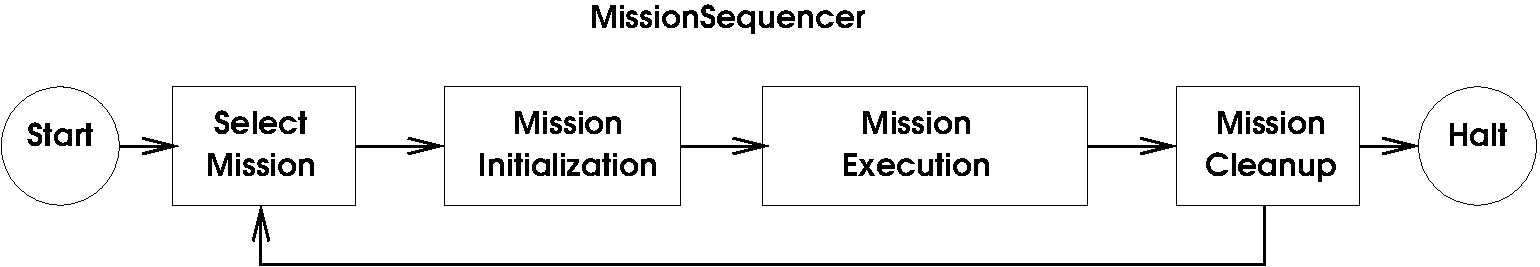
\includegraphics[width=\textwidth]{phases.pdf}
  \caption{A diagram showing the phases of SCJ mission execution}
  \label{phases-diagram}
\end{figure}

The first phase is initialisation, which consists of setting up the
schedulable objects controlled by the mission and creating any data
structures required for the mission.
Then the mission is executed by starting each of the schedulable
objects in the mission and waiting for a request to terminate the
mission.
When the mission is requested to terminate, each of the schedulable
objects in the mission is terminated and the mission's memory is
cleared.

The schedulable objects within a mission are asynchronous event
handlers that are released either periodically, at set intervals of
time, aperiodically, in response to a release request, or once at a
specific point in time (though handlers that are released once can
have a new release time set, allowing them to be released again).
At level 2 real-time threads are also allowed, which run continuously
from when they start until they finish, unless they are suspended or
interrupted by another schedulable object.

Each schedulable object has a priority and the highest priority object
that is eligible to run at each point in time is the object that runs.
This allows for simpler reasoning about order of execution and allows
for more urgent tasks to preempt less urgent tasks.

SCJ allows for assigning schedulable objects to ``scheduling
allocation domains'', where each domain consists of one or more
processors.
At Level 1, each scheduling allocation domain is restricted to a
single processor.
Hence, in scheduling terms, the system is fully partitioned.
This allows for mature single processor schedulability analysis to be
applied to each domain (although the calculation of the blocking times
when accessing global synchronised methods are different than they
would be on a single processor system due to the potential for remote
blocking~\cite{davis2011}).

SCJ deals with memory in terms of memory areas, which are Java objects
that provide an interface to blocks of physical memory called backing
stores.
Memory allocations in SCJ are performed in the backing store of the
memory area designated as the allocation context.
Each schedulable object has a memory area associated with it that is
used as the allocation context during a release of that object, and is
cleared after each release.
Each mission also has a mission memory area that can be used as an
allocation context by the schedulable objects of that mission, to
provide space for objects that need to persist for the duration of the
mission or to be shared between the schedulable objects.
The amount of memory required for the mission memory must be computed
ahead of time and specified by the programmer as part of writing the
mission, though there has been some work on automated computation of
worst case memory use for SCJ programs~\cite{andersen2013}.
There is also an immortal memory area where objects can be allocated
if needed for the entire running of the program (they are never
freed).
SCJ places restrictions on which objects an object may point to, so as
to avoid dangling pointers from being created.
Some examples of valid and invalid object references for some
asynchronous event handlers are shown in
Figure~\ref{stacks-areas-diagram}.

\begin{figure}[ht]
  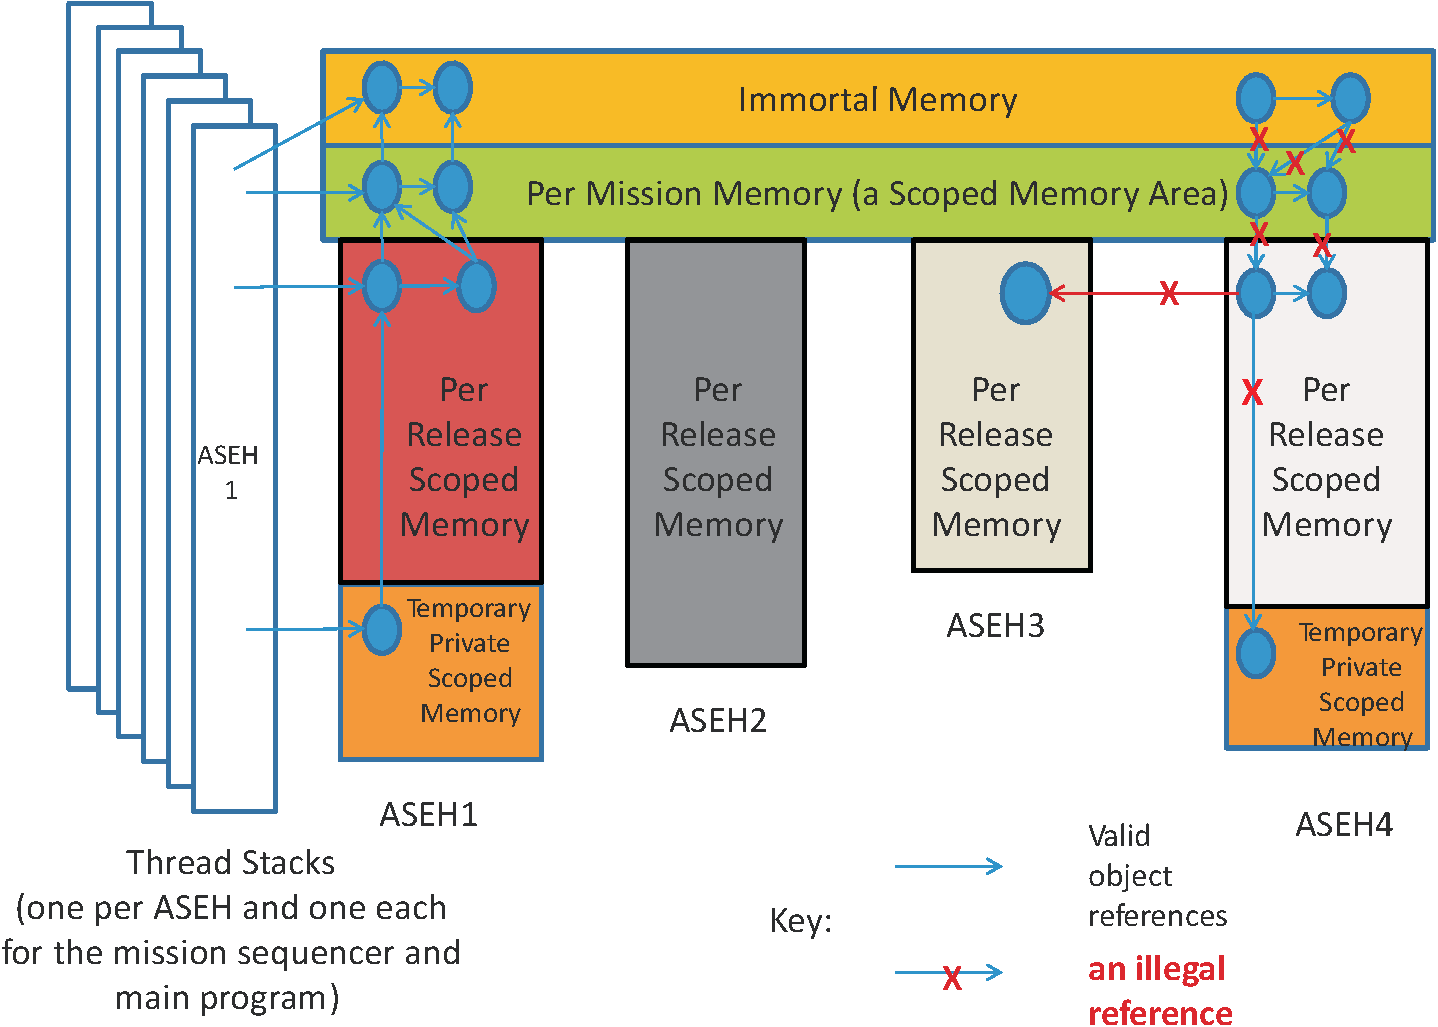
\includegraphics[width=\textwidth]{Stacks-Areas.pdf}
  \caption{An example of the layout of memory areas for four
    asynchronous event handlers (ASEHs), showing possible valid and
    invalid references between them}
  \label{stacks-areas-diagram}
\end{figure}

This system of memory areas makes it easy to predict when memory is
freed.
It is not supported by standard JVMs as they do not provide memory
outside of the heap for allocation and lack a notion of allocation
context.
The SCJ memory manager also needs to provide a means of accessing raw
memory for the purposes of device access, which is mediated by
accessor objects provided by the SCJ API.
As this API was stabilised at a later stage in the development of the
SCJ specification than its other features, we have not had opportunity
to include it in this work.
It can, however, be seen that any system of raw memory access is not
supported by most standard JVMs.

Moreover, dynamic class loading is not allowed in SCJ; all classes
used by the program must be loaded when the program starts.
This is because dynamic class loading may introduce time overheads
that are hard to predict and additional code paths that complicate
certification.
Finally, SCJ also disallows object finalisers as it is not always easy
to predict when they are run.

\section{Virtual Machines for Safety-Critical Java}
\label{virtual-machines-section}

% one subsection per machine

Because of the novel features of SCJ, briefly described in the
previous section, a specialised virtual machine that provides support
for allocation in memory areas and preemptive scheduling is required
for SCJ.
Although SCJ is a relatively recent development there have been
various virtual machines created for SCJ or variations of SCJ,
including icecap HVM~\cite{sondergaard2012}, Fiji VM~\cite{pizlo2009},
OVM~\cite{armbruster2007}, HVM\textsubscript{TP}~\cite{luckow2014} and
PERC Pico~\cite{atego2015, richard2010}.
These are each described in the following subsections.

\subsection{icecap HVM and
  \texorpdfstring{HVM\textsubscript{TP}}{HVMTP}}


The icecap hardware-near virtual machine (HVM) was created as part of
the Certifiable Java for Embedded Systems Project~\cite{schoeberl2014}
and provides an open-source implementation of SCJ targeted at embedded
systems.
The approach taken by the HVM is one of precompiling Java bytecode to
C in order to allow for faster running programs with fewer memory
resources.
It includes an implementation of the SCJ libraries that covers most of
SCJ level 2, originally supporting only single processor programs but
with multiprocessor support added later~\cite{zhao2015}.
This implementation, however, cannot be easily decoupled from the
virtual machine itself.

The icecap HVM also provides a lightweight Java bytecode interpreter
and allows for interpreted code to be mixed with compiled code.
The reason for this is that the bytecode together with the interpreter
can often be smaller than the compiled code, though there is a
tradeoff for speed.
HVM\textsubscript{TP} is a modification of the icecap HVM's bytecode
interpreter to improve time predictability and ensure that bytecode
instructions are executed in constant time, which is important for
ensuring real-time properties of the system hold.

\subsection{Fiji VM}

Fiji VM is a proprietary Java implementation designed to run on
real-time embedded systems.
Similarly to the icecap HVM, Fiji VM uses the strategy of compiling to
C in order to improve performance.
However, Fiji VM is not specifically targeted at SCJ and works with a
range of libraries, including SCJ, RTSJ and the standard Java
libraries.
Fiji VM does have the advantage of high portability and multiprocessor
support, which is lacking in some other SCJ virtual machines.

The fact that Fiji VM works with the SCJ libraries and supports the
scoped memory model means it can run SCJ programs.
It does not necessarily support all aspects of SCJ properly though.

\subsection{OVM}

OVM was created at Purdue University as part of the PCES
project~\cite{baker2006}, to provide a virtual machine that can
execute real-time Java programs with a high level of performance on
embedded systems.
Similar to Fiji VM and icecap HVM, OVM follows the principle of
precompiling code for performance reasons, but translates Java to C++
instead of bytecode to C.

OVM also differs from the icecap HVM and Fiji VM in that it predates
SCJ.
It is written to implement the RTSJ, though it can still support SCJ
programs; indeed, an SCJ implementation for OVM was later
created~\cite{plsek2010}.
However, OVM does not appear to have kept up with more recent changes
to the draft SCJ standard.
OVM is, unlike Fiji VM and the icecap HVM, single processor.

\subsection{PERC Pico}

PERC Pico is a product of Atego based on early ideas for SCJ, but uses
its own system of Java metadata annotations to ensure the safety of
scoped memory.
This systems of annotations provides additional information about how
memory is used so that it can be checked.
Similarly to other SCJ virtual machines, PERC Pico allows for
precompilation of Java code but targets executable machine code rather
than an intermediate programming language.
The metadata annotations are used to guide the compiler to produce
code that uses the correct scoped memory.
PERC Pico does not support the current SCJ standard, though it has
been suggested that it could be modified to do so~\cite{nilsen2011}.

To summarise, as far as we are aware there is one publicly available
virtual machine that has kept up with the developing SCJ
specification, the icecap HVM.
This is and, typically, virtual machines for SCJ will be, designed to
be very small and fast so as to be able to run on embedded systems.

As can be seen from the preceding discussion, a common technique to
run Java programs on embedded systems is to precompile them to native
code.
This means compiler correctness techniques must be considered in
verification of such a virtual machine; these techniques are discussed
in the next section.

\section{Compiler Correctness}
\label{compiler-correctness-section}

Due to the importance of compiler correctness, there has been much
research over the years in this area.
Most of the work done follows a similar approach, which we term
the commuting-diagram approach as it is based on showing that a
particular diagram commutes.
We discuss the commuting-diagram approach in
Section~\ref{commuting-diagram-subsection}.

An alternative approach to compiler verification is the algebraic
approach developed in the early 90s.
It is based on the concepts of refinement calculi designed for
deriving software from specifications of behaviour.
We explain the algebraic approach in
Section~\ref{algebraic-approach-subsection} and discuss how it differs
from the commuting-diagram approach.

We finish in Section~\ref{java-compiler-correctness-subsection} by
reviewing some of the literature on correctness of compilers for
Java-like languages.
We explain how the techniques of compiler correctness have been
applied in the case of Java and compare the different approaches.

\subsection{Commuting-diagram Approach}
\label{commuting-diagram-subsection}

Much of the work on compiler correctness can be seen as following the
approach identified by Lockwood Morris~\cite{morris1973}, and later
refined by Thatcher, Wagner and Wright~\cite{thatcher1979}.
The approach is essentially that a compiler correctness proof is a
proof that the diagram shown in Figure~\ref{commuting-diagram}
commutes, that is, $\gamma \circ \psi = \phi \circ \epsilon$.

\begin{figure}[ht]
  \begin{center}
    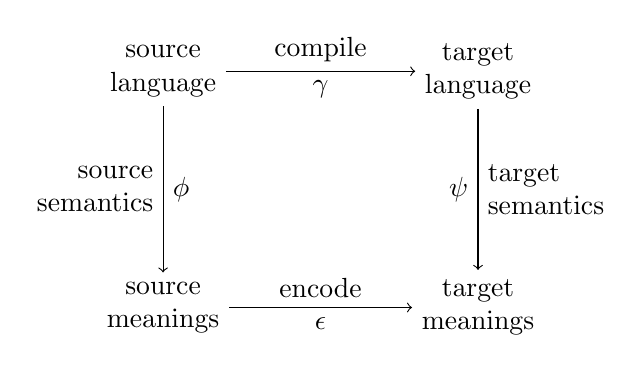
\begin{tikzpicture}
      \node[align=center] (S) at (0cm,3cm) {source\\language};
      \node[align=center] (T) at (4cm,3cm) {target\\language};
      \node[align=center] (M) at (0cm,0cm) {source\\meanings};
      \node[align=center] (U) at (4cm,0cm) {target\\meanings};
      
      \path (S) edge[->] node[align=center, above] {compile}
      node[align=center, below] {$\gamma$} (T); \path (S) edge[->]
      node[align=right, left] {source\\semantics}
      node[align=center,right] {$\phi$} (M); \path (T) edge[->]
      node[align=left, right] {target\\semantics} node[align=center,
      left] {$\psi$} (U); \path (M) edge[->] node[align=center, above]
      {encode} node[align=center, below] {$\epsilon$} (U);
    \end{tikzpicture}
  \end{center}
  \caption{The commuting diagram used in the traditional approach to
    compiler verification}
  \label{commuting-diagram}
\end{figure}

Lockwood Morris had the corners of the diagram as algebras, rather
than merely sets, with the functions between them being homomorphisms
in order to add additional structure to the proof.
This differs from the approach of some earlier works, particularly the
earliest work by McCarthy and Painter~\cite{mccarthy1967}, and instead
follows work such as that of Burstall and Landin~\cite{burstall1969}.

McCarthy and Painter's work featured a simple expression language with
addition, natural numbers and variables.
This was compiled to a simple 4-instruction single-register machine.
The arrows of the diagram were simple functions, rather than
homomorphisms, and the proof was performed using induction over the
source language.
This work laid the foundation for the study of compiler correctness.

Burstall and Landin showed correctness of a compiler for the same
source and target languages as McCarthy and Painter; they used a more
algebraic approach that better matches what Lockwood Morris later
suggested.
Burstall and Landin's approach involved representing the source and
target languages, and their meanings, as algebras, with the
compilation functions as homomorphisms.
They targeted several intermediate machines in the proof of
correctness.
Viewing the languages as algebras allows for simpler proofs as some of
the arrows of the commuting diagram can be wholly or partially derived
from the algebraic structure.
It was this goal of simplifying the proofs that led Lockwood Morris to
advocate the use of algebras and homomorphisms.

The overall goal of pursuing formal proofs of compiler correctness, as
proposed by McCarthy and Painter~\cite{mccarthy1967}, is to allow
machine-checked proofs of program correctness.
There has been work in that area, the earliest of which was that by
Milner and Weyhrauch~\cite{milner1972} who showed the correctness of
an ALGOL-like language.
The proof of correctness was partially mechanised in the LCF theorem
prover~\cite{milner1972a} and the authors were of the opinion that the
proof was feasible and could be completed relatively easily.
A point to note is that Milner and Weyhrauch acknowledged the need for
some way of structuring the proof in order to make it amenable to
machine-checking.
This gives further support to the algebraic commuting-diagram approach
advocated by Lockwood Morris.
Indeed, Milner and Weyhrauch explicitly followed that approach as they
were in discussions with Lockwood Morris.

One advantage to making proofs easily machine-checkable, apart from
the added certainty that the proof is correct, is that working
compilers can be created from the machine-checked proofs.
Code generation facilities are available with many theorem provers
such as those of Isabelle/HOL~\cite{haftmann2007} and
Coq~\cite{letouzey2003, letouzey2008}.
The fact that the commuting-diagram approach involves treating the
compilation as a function between algebras representing the source and
target languages fits well with this idea.
In this case, there is then a function defined in the mechanised logic
for the purposes of conducting proofs about it that can be readily
extracted to executable code.

The commuting-diagram approach has been followed in much of the
literature through the years, though not always with the algebraic
methods recommended by Lockwood Morris.
The basic structure of the commuting diagram is a fairly natural
approach to take, as seen by work such as that of the ProCoS
project~\cite{buth1992}.

Another piece of work that follows the commuting-diagram approach is
that of Polak~\cite{polak1981}, who states that he is more interested
in verification of a ``real'' compiler rather than ``abstract code
generating algorithms'', and shows the correctness of a compiler for a
Pascal-like language.
This work focuses much more on pragmatic applications of the
commuting-diagram approach, leaving behind the algebraic ideas of
earlier papers.
It sets a precedent for a simpler verification approach based on
considering the functions in the commuting diagram.

The commuting-diagram approach has also been used in recent work, some of the
most successful of which is that of CompCert~\cite{leroy2009a,
  leroy2009b, leroy2012}.
This is a project to create a fully verified realistic compiler for a
subset of C, using the theorem prover Coq~\cite{coq2004}.

There is also recent variation of the commuting-diagram approach, 
based on an operational semantics of the source
language~\cite{bahr2015}.
In this work, the operational semantics of the source language and
a way of relating the source and target semantics are used to derive a
different operational semantics of the source language acting on the
state of the target machine.
The semantics of the target language are then identified as part of
that operational semantics and it is transformed to extract a
compilation function.
This approach may be viewed as variant of the commuting-diagram
approach in which the compilation function is derived from the source
and target semantics and the relationship between them, rather than
being verified by those elements of the commuting diagram.

\subsection{Algebraic Approach}
\label{algebraic-approach-subsection}

The second main approach to showing correctness of compilers is the
algebraic approach proposed by Hoare in 1991~\cite{hoare1991}, and
further developed by Sampaio~\cite{hoare1993, sampaio1993,
  sampaio1997}.
We note that the algebraic approach discussed in this section is
largely unrelated to the algebraic commuting-diagram approaches
mentioned in the previous section.

The algebraic approach to compilation derives from the concepts of
algebraic reasoning about programs and program refinement.
These concepts come from the idea, proposed by Hoare in
1984~\cite{hoare1984}, that programs can be thought of as predicates
and so the laws of predicate logic can be used to construct laws for
reasoning about programs~\cite{hoare1987}.
As an example of such a law for reasoning about programs, we present
below associativity of sequential composition,
Equation~\eqref{seq-comp-assoc}, and left and right unit of sequential
composition, namely, the program $\Skip$ that does nothing,
Equation~\eqref{skip-comp-identity}.
\begin{equation}
  \label{seq-comp-assoc}
  P;(Q;R) = (P;Q);R
\end{equation}
\begin{equation}
  \label{skip-comp-identity}
  P;\Skip = \Skip;P = P
\end{equation}

The notion of refinement is central to the algebraic approach to
compilation.
Refinement calculi have been developed, independently, by
Back~\cite{back1981}, Morris~\cite{morris1987} and
Morgan~\cite{morgan1990}, following from earlier concepts of program
transformation~\cite{bauer1976, balzer1976, standish1976, arsac1979}.
The basic idea is that there is a relation between programs that
captures the idea of one program being ``at least as good as'' another
or, to put it more precisely, at least as deterministic as another.
Languages and laws for reasoning about programs with this notion of
refinement can then be used to develop programs from specifications.
This means that certain aspects of a system can have a
nondeterministic specification and several different implementations
can refine that specification.

In using refinement to show the correctness of a compiler, the laws of
the specification language can be used to prove compilation refinement
laws.
These compilation laws can be used to transform the source programs
into some normal form that represents an interpreter for the target
language running the target code.
In other words, the code output by the compiler, when executed by on
the target machine, must be a refinement of the source program.
The compilation laws can be used to prove this refinement and at the
same time generate the target code.

As an example, consider the following refinement in which a simple
program that performs some arithmetic and stores the results into
variables is refined by a normal form representing the target machine
and code.
The symbol $\circrefines$ represents the refinement relation here.
\begin{equation}
  \circvar x, y, z \circspot x := (x + 5) \times (y + z) ; z := z + 1
  \circrefines
  \begin{aligned}
    &\circvar A, P, M \circspot P := 1; \circdo \\
    &\quad            P=1  \then A,    P := M[2],          2 \\
    &\quad \extchoice P=2  \then A,    P := A + M[3],      3 \\
    &\quad \extchoice P=3  \then M[4], P := A,             4 \\
    &\quad \extchoice P=4  \then A,    P := M[1],          5 \\
    &\quad \extchoice P=5  \then A,    P := A + 5,         6 \\
    &\quad \extchoice P=6  \then A,    P := A \times M[4], 7 \\
    &\quad \extchoice P=7  \then M[1], P := A,             8 \\
    &\quad \extchoice P=8  \then A,    P := M[3],          9 \\
    &\quad \extchoice P=9  \then A,    P := A + 1,         10 \\
    &\quad \extchoice P=10 \then M[3] := A,                11 \\
    &\circod ; \{ P = 11 \}
  \end{aligned}
\end{equation}
The normal form represents the behaviour of an interpreter for the
target code running in a target machine whose structure is defined
by the variables A, P, and M.
The variable $A$ represents a general-purpose register of the target
machine, $P$ represents the program counter of the target machine, and
$M$ is an array representing the memory of the target machine.
The normal form consists of a program that initialises $P$ to 1 and
then enters a loop in which the operation performed on each iteration
is dependent on the value of $P$.
The loop is exited when $P$ is set to a value for which there is no
operation and it is asserted that $P$ will be equal to 11 at the end
of the program.
Each of the statements of the source program corresponds to several
operations in the normal form as complex expressions are broken down
into simpler expressions that can be handled by instructions of the
target machine.

The compilation proceeds by first applying rules to simplify the
assignment statements.
The register $A$ is introduced at this stage by splitting assignments
of expressions to variables into two assignments that transfer the
values to and from $A$.
In this way, the assignments are transformed for the target machine
that only has instructions involving registers.
Particularly complex expressions such as $(x + 5) \times (y + z)$ are
handled by storing intermediate results in temporary variables.
In this case the result of the expression $y + z$ is placed in a
temporary variable when $P = 3$.
The variables used in the source program and introduced compilation
are later replaced with locations in the memory array $M$ in a data
refinement step.
This causes the variables $x$, $y$ and $z$ to be replaced with $M[1]$,
$M[2]$ and $M[3]$ respectively.
The temporary variable introduced to store the result of $y + z$ is
similarly replaced with $M[4]$.

Each of the assignment statements is then refined by a normal form
with an explicit program counter $P$, that is incremented as part of
the assignment operation.
These normal forms are then combined together by the refinement rule
for sequential composition to create the normal form of the full
program.
The update of the program counter in this program is quite simple but
more complex updates would occur for conditionals or loops.

The power of the algebraic approach is that the compilation of
individual elements of the source language can be specified and proved
separately in different refinement laws.
The compilation can also be split into stages, with a set of
refinement laws for each stage to modularise the compilation.
The separate refinement laws can then be combined to form a
compilation strategy.

The first major work done using the algebraic approach was that of
Sampaio~\cite{sampaio1993}, who used it to specify a correct compiler
for a simple language that, nonetheless, covers all the constructs
available in most programming languages.
The target machine Sampaio used was a simple single-register machine
that bears similarity to most real processor architectures.
He mechanised the compiler in the OBJ3 term rewriting
system~\cite{goguen1988}, showing that working compilers can be easily
created from specifications using the algebraic approach.
However, the algebraic laws Sampaio used to prove correctness of the
compiler were taken as axioms.
Sampaio notes that they could be easily proved given a semantics for
the reasoning language.

Though there has not been much work done using the algebraic approach,
we single out the work of Perna~\cite{perna2010, perna2011}, showing
correctness of a compiler for a hardware description language.
The compilation takes high-level descriptions of hardware written in
Handel-C and transforms them into systems of basic hardware components
connected by wires.
The algebraic approach works well here as the target language is a
subset of the source language, albeit in a different form.
Perna was able to handle features not covered by most other works on
hardware compilation, such as parallelism with shared variables.
Also, whereas Sampaio took the basic algebraic laws as axioms, Perna
proved the laws from a semantics given using the Unifying Theories of
Programming (UTP) model~\cite{hoare1998}.
There has also been work on the correctness of Java compilers using
the algebraic approach.
This is considered in the next section, where we consider compiler
correctness for Java-like languages.

\subsection{Correctness of Java Compilers}
\label{java-compiler-correctness-subsection}

The popularity of Java has meant that there has been plenty of work on
formalising Java and the JVM~\cite{hartel2001}, but there have been
relatively few works on formally verified compilers for Java-like
languages.
However, the work that has been done uses both of the two main
approaches and covers most of the features of Java.

Some of the earliest and most thorough work is that by S\"{a}rk,
Schmid and B\"{o}rger~\cite{stark2001}, who formalise most of Java and
the JVM before specifying and showing the correctness of a compiler
for Java.
The approach taken by them uses Abstract State Machines (ASMs) to
specify the source and target languages.
The ASMs give an operational semantics to Java and the JVM, describing
how each construct affects the running of the program.
The languages are each specified by multiple ASMs, beginning with an
imperative core, then adding classes, objects, exceptions and,
finally, threads.

Although this approach is called the ASM approach, it becomes clear
from the definition of compiler correctness given in terms of a
mapping between ASMs that this work ultimately follows the
commuting-diagram approach.
This work leaves parts of the proof incomplete (in particular,
compilation of threads is not addressed) and applies to an old version
of Java.
This is, nevertheless, an admirable attempt at producing a verified
Java compiler.

Work has also been done by Duran following the algebraic
approach~\cite{duran2005, duran2010}.
Duran's work specifies a compiler for a language called Refinement
Object-Oriented Language (ROOL)~\cite{borba2000}, which was created
for reasoning about object-oriented languages and bears much
similarity to Java.
ROOL features constructs for specifying and reasoning about programs
as well as object-oriented programming language constructs.
This means that the there are algebraic laws for ROOL, from which the
rewrite rules that form the basis of the algebraic approach can be
proved.
Duran's work adds further phases to Sampaio's compilation strategy in
order to deal with the object-oriented features, but does not consider
some other aspects of Java such as exceptions and threads.
Duran notes that other work has addressed some of those issues.

While the two works already discussed were not machine checked, there
have also been compiler correctness proofs for Java-like languages in
the Isabelle/HOL proof assistant.
The first of these was by Strecker~\cite{strecker2002}, showing
correctness of a compiler for a subset of Java called $\mu$Java, which
already had a formalisation of its semantics in
Isabelle/HOL~\cite{nipkow2000}.
This work was followed by Klein and Nipkow's work on a compiler for a
slightly larger subset of Java called Jinja~\cite{klein2006}, which
added exception handling.
Finally, Lochbihler~\cite{lochbihler2010} added threads to Jinja and
showed correctness of compilation for Java concurrency.
It is notable that this is the only work on Java compilation that
properly addresses concurrency.
All of these works follow the commuting-diagram approach.

Though some work has been done on correct compilers for Java-like
languages and many virtual machines for SCJ adopt an approach of
compiling to native code, no work has been done on verifying that
compilation to native code.
Therefore, in this thesis, we consider correctness of the compilation
to native code as part of our work on SCJ virtual machines.
We follow the algebraic approach as it gives greater assurance of
correctness, as an additional function mapping source meanings to
target meanings is not required, and a good level of modularity, as
the compilation is split into separately proved rewrite rules.
In order to represent the normal form we require a specification
language and for that purpose use \Circus{}, which is described
in the next section.

\section{\Circus{}}
\label{circus-section}

The \Circus{} specification language~\cite{oliveira2009} is based on
CSP~\cite{roscoe2011}, which is used to specify processes that
communicate over channels, and the Z notation~\cite{woodcock1996},
which is used to specify state and data operations.
A \Circus{} specification is made up of processes that communicate
over channels.
These channels may carry values of a particular type, or may be used
as flags for synchronisation or signalling between processes.
Each process may have state, and is made up of actions that operate on
that state and communicate over channels.

We illustrate the concepts of \Circus{} using as an example the
process for the real-time clock from an early version of our
specification of an SCJ virtual machine.
The specification begins with a declaration of the channels that may
be used in the following processes.
Type declarations written in Z can also be included at the beginning
of a \Circus{} specification.
Here, we define a type $Time$ to be the set of natural numbers and
create a boolean datatype
%
\begin{zed}
  Time == \nat \\
  Bool ::= True | False
\end{zed}
%
We declare channels to represent interactions corresponding to calls
to methods to get the clock's time and precision, and set and clear
alarms.
Channels are also declared to model interactions with the hardware
that accept clock tick interrupts and read the time from the hardware
clock.
%
\begin{circus}
  \circchannel getTime, getPrecision, setAlarm : Time \\
  \circchannel clearAlarm \\
  \circchannel HWtick \\
  \circchannel HWtime : Time
\end{circus}
%
We also specify a constant to represent the clock's precision using a
Z axiomatic definition.
The value of the constant is required to be nonzero, but is otherwise
left unrestricted, so that any nonzero time value is a valid
instantiation.
%
\begin{axdef}
  precision : Time \where precision > 0
\end{axdef}
%
After the channel declarations, we can declare processes that use
them.
Here we declare the $RealtimeClock$ process.
It is a basic process, that is, its state is defined in Z, and its
behaviour using CSP constructs and Z data operations.
%
\begin{circus}
  \circprocess RealtimeClock \circdef \circbegin
\end{circus}
%
In this example, the state records the current time, whether an alarm
is set, and the time of the alarm that may be set.
An invariant specifies that if an alarm is set, then the time of the
alarm must not be in the past.
%
\begin{schema}{RTCState}
  currentTime  : Time \\
  alarmSet     : Bool \\
  currentAlarm : Time
\where
  alarmSet = True \implies \\
  \t1 currentAlarm \geq currentTime
\end{schema}
\begin{circusaction}
  \circstate RTCState
\end{circusaction}
%
The behaviour is described using actions, written in a mixture of Z
and CSP.
The first action is a Z initialisation operation, $Init0$.
Its final state is represented by variables obtained by placing a
prime on the names of the state components.
Here, the initialisation takes as input the initial time, represented
by the variable $initTime?$.
In Z schemas, inputs to operations are distinguished by ending with a
question mark.
Similarly, outputs are marked with an exclamation mark.
The current time is defined to be equal to the initial time and no
alarm is initially set.
The initial time of the alarm is arbitrary, that is,
nondeterministically chosen from elements of its type, since the
initialisation imposes no restrictions on it.
%
\begin{schema}{Init0}
  RTCState~' \\
  initTime? : Time
\where 
  currentTime' = initTime? \\
  alarmSet' = False
\end{schema}
%
The action $Init$, defined below, uses a CSP prefixing to specify an
input communication before the initialisation operation $Init0$.
The initial time of the clock is read from the hardware clock and then
the initialisation specified by the Z schema is performed.
%
\begin{circusaction}
  Init \circdef HWtime?initTime \then Init0
\end{circusaction}
%
The action that returns the current time simply uses CSP to output the
current time from the state over the $getTime$ channel.
The action ends with the special action $\Skip$, which indicates the
end of an action.
%
\begin{circusaction}
  GetTime \circdef getTime!currentTime \then \Skip
\end{circusaction}
%
Setting a new alarm is a more complex operation that involves Z
schemas that specify two different scenarios in which this operation
may be used.
In the first case, the new alarm is not in the past.
The symbol $\Delta$ denotes a change of state.
The operation stores the time of the new alarm and sets a flag to
indicate an alarm is set in this case.
%
\begin{schema}{SetAlarm0}
  \Delta RTCState \\
  newAlarm? : Time
\where
  newAlarm? \geq currentTime \\
  currentAlarm' = newAlarm?{} \\
  alarmSet' = True \\
  currentTime' = currentTime
\end{schema}
%
In the second case, the new alarm is in the past and so the alarm is
not set (we have omitted the error reporting for the sake of
simplicity).
The symbol $\Xi$ denotes that the state remains the same.
%
\begin{schema}{SetAlarm1}
  \Xi RTCState \\
  newAlarm? : Time
\where
  newAlarm? < currentTime
\end{schema}
%
The two Z schemas are combined using a logical disjunction, allowing
either to specify the behaviour when a request to set the alarm takes
place.
%
\begin{circusaction}
  SetAlarm \circdef setAlarm?newAlarm \then \lschexpract SetAlarm0 \lor SetAlarm1 \rschexpract
\end{circusaction}
%
In addition to Z and CSP constructs, \Circus{} also has other
constructs more familiar to programmers, such as if statements and do
loops.
One of these constructs, the assignment operator, is used in the
action that clears the current alarm to update part of the state
without requiring a Z schema.
The alarm is cleared by simply setting $alarmSet$ to $False$, without
updating any other state variables.
%
\begin{circusaction}
  ClearAlarm \circdef clearAlarm \then alarmSet := False
\end{circusaction}
%
Each of the actions the process can perform are joined together with
the CSP external choice operator, which chooses an action to take
based on the channel communications that the environment is willing to
perform.
This includes the actions above, as well as some other actions that
have been omitted here.
The choice is repeated in a loop.
%
\begin{circusaction}
  Loop \circdef \left( GetTime \extchoice SetAlarm \extchoice
    ClearAlarm
    \extchoice \cdots \right) \\
  \t1 \circseq Loop
\end{circusaction}
%
The \Circus{} process then ends with the main action that specifies
the overall behaviour of the process.
Here, the process simply performs the initialisation and then enters
the loop.
%
\begin{circusaction}
  \circspot Init \circseq Loop
\end{circusaction}
\begin{circus}
  \circend
\end{circus}

In addition to the constructs presented here \Circus{} also contains
operators for composing processes in parallel, with or without
synchronisation on channels.
These operators are used both to specify actual parallelism and to
represent composition of requirements.
In this way several \Circus{} specifications of individual components
can be combined to form a specification of the entire system.

A detailed account of \Circus{} can be found in~\cite{oliveira2009}.
Table~\ref{circus-operators-table} summarises the \Circus{} constructs
used in this thesis.

\begin{table}
  \centering
  \begin{tabular}{p{11.3cm}l}
    \hline
    Construct & \Circus{} notation \\
    \hline
    Termination & $\Skip$ \\
    Divergence (abortion) & $\Chaos$ \\
    Assignment of expression $e$ to variable $x$ & $x := e$ \\
    Prefixing of signal on channel $c$ to action $A$ & $c \then A$ \\
    Prefixing of output on channel $c$ of expression $e$ to action $A$ & $c!e \then A$ \\
    Prefixing of input on channel $c$ of variable $x$ to action $A$ & $c?x \then A$ \\
    Variable block with variable $x$, of type $T$, and action $A$ & $\circvar x : T \circspot A$ \\
    Value parameter block with parameter $x$, of type $T$, and action $A$ & $\circval x : T \circspot A$ \\
    Result parameter block with parameter $x$, of type $T$, and action $A$ & $\circres x : T \circspot A$ \\
    Instantiation of parameterised action $A$ with expression $e$ & $A(e)$ \\
    Guarding of $A$ with predicate $g$ & $\lcircguard g \rcircguard \circguard A$ \\
    Sequential composition of actions $A$ and $B$ & $A \circseq B$ \\
    External choice of actions $A$ and $B$ & $A \extchoice B$ \\
    Conditional choice of actions $A$ and $B$, with conditions $g$ and $h$ & $\circif g \circthen A \circelse h \circthen B \circfi$ \\
    Parallel interleaving of processes $P$ and $Q$ & $P \interleave Q$ \\
    Recursion with body given by action function $F$ & $\circmu X \circspot F(X)$ \\
    Parallel composition of processes $P$ and $Q$, synchronising on the \endgraf \hspace{1cm} intersection of channel sets $cs1$ and $cs2$ & $P _{cs1}\!\!\parallel_{cs2} Q$ \\
    Parallel composition of processes $P$ and $Q$, synchronising on the \endgraf \hspace{1cm} channel set $cs$ & $P \lpar cs \rpar Q$ \\
    Hiding of channel set $cs$ in process $P$ & $P \circhide cs$ \\
    \hline
  \end{tabular}
  \caption{Summary of \Circus{} notation}
  \label{circus-operators-table}
\end{table}

% for the thesis add a more comprehensive description of Circus with a
% description of process operators and tables of operator descriptions

\section{Final Considerations}
\label{final-considerations-section}

% summarise the problem and how to solve it

We have seen that Java is increasingly being considered as a language
for safety-critical embedded systems and that the modifications to
Java required to make it suitable for such systems require a
specialised virtual machine.
The developing Safety-Critical Java specification has several
differences from standard Java, particularly in the areas of
scheduling and memory management, that make standard JVMs unsuitable
for running SCJ programs.
We have considered several virtual machines that have been developed
for running SCJ programs and noted that none of them has been formally
verified and that most of them adopt an approach of precompiling
programs to native code.

With that in mind, we have considered the techniques used to verify
the correctness of compilers and found that there are two main
approaches: the commuting-diagram approach and the algebraic approach.
In the commuting-diagram approach the source semantics, target
semantics, compilation function, and a function mapping the source
meanings to the target meanings, are shown to commute.
This approach is popular and has had much research done on it but
relies on the definition of the function from the source meanings to
the target meanings.

The algebraic approach defines the source and target languages within
the same specification language, which is additionally equipped with a
refinement relation between programs.
Laws of the specification language are then used to prove refinement
rules that are applied according to some compilation strategy.
The algebraic approach has the advantage that it does not require the
additional function that is required in the commuting-diagram
approach, since the source and target languages are defined in terms
of the same specification language.
The algebraic approach also permits a modular approach to proof and
allows for the compiler to be easily implemented by application of the
refinement rules using a term rewriting system.

Given the considerations above, we have decided to adopt the algebraic
approach when specifying the compilation to native code employed by
many SCJ virtual machines.
This means that a specification language is required in which to
define the source and target languages, as well as for the purposes of
specifying other aspects of the virtual machine.
We have chosen \Circus{} as the specification language as it contains
a wide variety of constructs that allow for specification of both data
and behaviour, has a well defined semantics with many laws already
proved, and has been used for previous work on the specification of
SCJ programs.
\Circus{} also has some existing mechanisation and tool support, which
can help give greater assurance of the correctness of specifications.

\chapter{Safety-Critical Java Virtual Machine Services}
\label{scjvm-services-chapter}

In order to reason about a Safety-Critical Java virtual machine
(SCJVM), we first require an identification of the the requirements of
an SCJVM and a formal model of those requirements.
For the purposes of our model, we consider an SCJVM to have the
components illustrated in Figure~\ref{scjvm-services-fig}.
An SCJVM is divided into two main parts:~the core execution
environment and the SCJVM services that may make use of the services
of an underlying operating system or hardware abstraction layer.

\begin{figure}[ht]
  \centering
  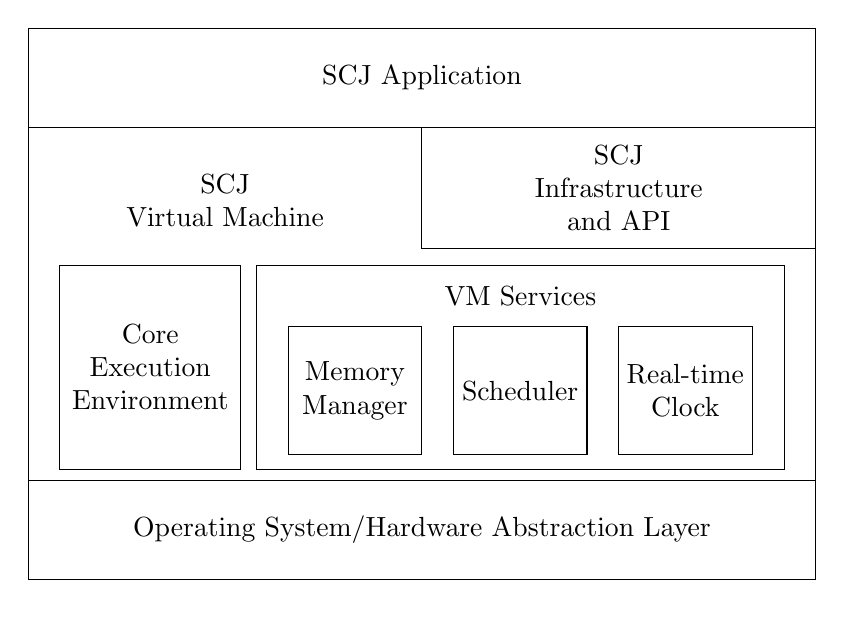
\begin{tikzpicture}

    \coordinate (width)  at (10cm,0cm);
    \coordinate (height) at (0cm,7cm);

    \path (0,0) -- (height)
    coordinate[pos=0.18] (OS boundary)
    coordinate[pos=0.20] (VM part bottom)
    coordinate[pos=0.57] (VM part top)
    coordinate[pos=0.60] (API boundary)
    coordinate[pos=0.82] (App boundary);
    
    \path (VM part bottom) -- (VM part top)
    coordinate[pos=0.7] (VM Service top);

    \path (VM part bottom) -- (VM part top)
    coordinate[pos=0.85] (VM Services ypos);

    \path (0,0) -- (width)
    coordinate[pos=0.04] (CEE left)
    coordinate[pos=0.27] (CEE right)
    coordinate[pos=0.29] (VM Services left)
    coordinate[pos=0.96] (VM Services right)
    coordinate[pos=0.17] (VM Service width)
    coordinate[pos=0.04] (VM Service sep);

    \path (VM Services left) -- (VM Services right)
    coordinate[pos=0.5] (VM Services xpos);

    \path (0,0) to node[pos=0.5] (mid) {} (width);
    \path (0,0) to node[pos=0.25] (quart) {} (width);

    \draw (0,0) rectangle (width |- height);

    \draw (OS boundary) -- ++(width);
    \path (0,0) rectangle node[pos=0.5] (OS) {} (width |- OS boundary);
    \draw (mid |- API boundary) rectangle node[pos=0.5] (API) {} (width |- App boundary);
    \draw (App boundary) -- ++(width);
    \path (App boundary) rectangle node[pos=0.5] (App) {} (width |- height);

    \path (quart |- API boundary) rectangle node[pos=0.4] (SCJVM) {} (quart |- App boundary);
    \draw (CEE left |- VM part bottom) rectangle node[pos=0.5] (CEE) {} (CEE right |- VM part top);
    \draw (VM Services left |- VM part bottom) rectangle (VM Services right |- VM part top);
    \coordinate (VM Services) at (VM Services xpos |- VM Services ypos);

    \node[align=center] at (App)   {SCJ Application};
    \node[align=center] at (API)   {SCJ\\Infrastructure\\and API};
    \node[align=center] at (SCJVM) {SCJ\\Virtual Machine};
    \node[align=center] at (CEE)   {Core\\Execution\\Environment};
    \node[align=center] at (OS)    {Operating System/Hardware Abstraction Layer};
    
    \foreach \x in {1,...,3}
    \pgfmathsetmacro{\a}{0.333*(\x - 1)}
    \pgfmathsetmacro{\b}{0.333*\x}
    \path ($(VM Services left) + (VM part bottom)!0.07!(VM part top)$) -- 
    node[pos=\a] (VM Service \x start) {}
    node[pos=\b] (VM Service \x end) {}
    ($(VM Services right) + (VM part bottom)!0.07!(VM part top) - (VM Service sep)$);

    \foreach \x in {1,...,3} 
    \draw ($(VM Service \x start) + (VM Service sep)$)
    rectangle node[pos=0.5] (VM Service \x) {}
    (VM Service \x end |- VM Service top);

    \node[align=center] at (VM Services)  {VM Services};
    \node[align=center] at (VM Service 1) {Memory\\Manager};
    \node[align=center] at (VM Service 2) {Scheduler};
    \node[align=center] at (VM Service 3) {Real-time\\Clock};
  \end{tikzpicture}
  \caption{A diagram showing the structure of an SCJVM and its
    relation to the SCJ infrastructure and the operating
    system/hardware abstraction layer, focusing on the SCJVM services}
  \label{scjvm-services-fig}
\end{figure}

The core execution environment manages the execution of Java bytecode,
whether that be via interpretation, just-in-time compilation or
ahead-of-time compilation.
The core execution environment must also manage data that relates to
the execution of bytecode instructions, such as the representation of
classes and objects.

The SCJVM services represent the additional services that must be
offered by an SCJVM in order to support the SCJ infrastructure.
These services may be supplied as standalone services and so do not
need to be handled by the compilation strategy.
We consider the virtual machine services to be divided into three
areas:
\begin{itemize}
\item the memory manager, which manages backing stores for memory areas and
  allocation within them;
\item the scheduler, which manages threads and interrupts, and allows for
  implementation of SCJ event handlers; and
\item the real-time clock, which provides an interface to the system real-time
  clock.
\end{itemize}
Each of these services is used either by the core execution environment or by
the SCJ infrastructure; some of the services also rely on each other.  For
example, the scheduler must update the allocation context in the memory manager
when performing a thread switch.

A model of the core execution environment is presented in
Chapter~\ref{cee-chapter}.
In this chapter, we present the requirements for each area of the
SCJVM services:~the memory manager in
Section~\ref{memory-manager-section}, the scheduler in
Section~\ref{scheduler-section}, and the real-time clock in
Section~\ref{realtime-clock-section}.
The formal model of the SCJVM requirements is presented in
Section~\ref{formal-model-section}.
A complete version of the model can be found in
Appendix~\ref{full-scjvm-services-model}

The memory manager model has been subject to proof using Z/Eves.
The theorems proved about the memory manager can be found in
Appendix~\ref{memory-manager-theorems}, with the Z/Eves proof scripts
in Appendix~\ref{memory-manager-proofs}.
Many additional lemmas about objects in the Z/Eves mathematical
toolkit have been proved in the course of carrying out these proofs.
As these can be of use outside our work, we have included them
separately in Appendix~\ref{additional-lemmas} with their proofs in
Appendix~\ref{additional-lemmas-proofs}.

Part of an earlier version of this model was presented at the 13th
International Workshop on Java Technologies for Real-time and Embedded
Systems~\cite{baxter2015a} with the full earlier version made available
as a technical report~\cite{baxter2015}.

\section{Memory Manager API}
\label{memory-manager-section}

The SCJVM memory manager deals with the raw blocks of memory used as
backing stores for the memory areas of SCJ.
The memory areas themselves are Java objects, and so are dealt with by
the core execution environment and accessed through the SCJ API,
instead of directly via the virtual machine.
This is in line with what is specified in the SCJ standard and also
done for RTSJ.
Backing stores are assumed to have unique identifiers that can be used
to refer to them; these identifiers can be simply pointers to the
physical blocks of memory used for backing stores.

There is initially one backing store, called the root backing store,
which has its size set when the SCJVM starts up to cover all the
memory available for allocation in backing stores.
The root backing store cannot be resized or destroyed, so that there
is always a fixed base for the layout of memory.
The root backing store is used as the backing store for the immortal
memory area.

A backing store may have other backing stores nested within it, so
that a possible memory layout is as shown in Figure~\ref{memory-fig}.
In this example, the backing store of the mission memory is nested
within the root backing store, and the backing stores for the
per-release memory of each schedulable object in a mission is nested
within the mission memory's backing store.

\begin{figure*}[ht]
  \centering
  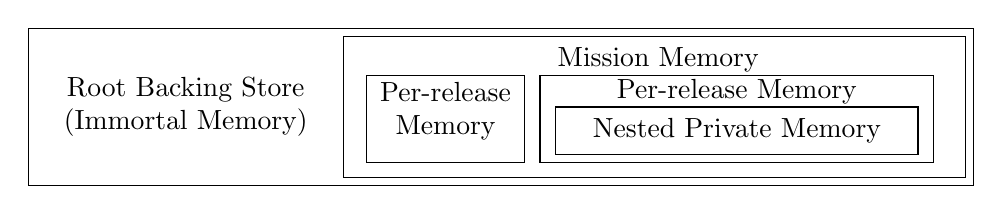
\begin{tikzpicture}
    \draw (0,0) rectangle (12,2); \node[align=center] at (2,1) {Root
      Backing Store\\(Immortal Memory)};
    
    \draw (4,0.1) rectangle (11.9,1.9); \node[align=center] at (8,1.6)
    {Mission Memory};
    
    \draw (4.3,0.3) rectangle (6.3,1.4); \node[align=center] at
    (5.3,0.95) {Per-release\\Memory};
    
    \draw (6.5,0.3) rectangle (11.5,1.4); \node[align=center] at
    (9,1.2) {Per-release Memory};
    
    \draw (6.7,0.4) rectangle (11.3,1); \node[align=center] at (9,0.7)
    {Nested Private Memory};
  \end{tikzpicture}
  \caption{An example memory layout}
  \label{memory-fig}
\end{figure*}

The operations of the memory manager API are summarised in
Table~\ref{memory-manager-table}.
In addition to the inputs and outputs described there, there should
also be some system of reporting erroneous inputs, whether that be
exceptions, global error flags, or particular return values signalling
errors.
The conditions that cause an error to be reported are listed in
Table~\ref{memory-manager-table} as well.

\begin{table*}[ht]
  \centering
  \footnotesize
  \begin{tabular}{|l|p{3.1cm}|p{3.1cm}|p{3.9cm}|}
    Operation & Inputs & Outputs & Error Conditions \\
    \hline
    \texttt{getRootBackingStore} &
    (none) &
    backing store identifier &
    (none)
    \\\texttt{getTotalSize} &
    backing store identifier &
    size in bytes &
    invalid identifier
    \\\texttt{getUsedSize} &
    backing store identifier &
    size in bytes &
    invalid identifier
    \\\texttt{getFreeSize} &
    backing store identifier &
    size in bytes &
    invalid identifier
    \\\texttt{findBackingStore} &
    memory pointer &
    backing store identifier &
    no backing store found
    \\\texttt{allocateMemory} &
    backing store identifier \newline
    size in bytes &
    memory pointer &
    invalid identifier \newline
    insufficient free memory \newline
    no current allocation context
    \\\texttt{makeBackingStore} &
    backing store identifier \newline
    size in bytes & 
    backing store identifier &
    invalid identifier \newline
    insufficient free memory
    \\\texttt{clearBackingStore} &
    backing store identifier &
    (none) &
    invalid identifier \newline
    nested backing store in use
    \\\texttt{resizeBackingStore} &
    backing store identifier \newline
    size in bytes &
    backing store identifier &
    invalid identifier \newline
    backing store in use \newline
    backing store is root \newline
    backing store not empty \newline
    backing store not only child \newline
    insufficient free space \newline
    no space for memory overhead
    \\\texttt{createStack} &
    size in bytes &
    stack identifier &
    insufficient free space
    \\\texttt{destroyStack} &
    stack identifier &
    (none) &
    invalid identifier \newline
    stack space fragmentation
  \end{tabular}
  \caption{The operations of the SCJVM memory manager}
  \label{memory-manager-table}
\end{table*}

The root backing store is always available to the SCJ infrastructure
through the \texttt{get\-Root\-Backing\-Store} operation.
An SCJ program, on the other hand, does not have direct access to the
root backing store except through memory areas provided by the
infrastructure.

It is possible to obtain information about the used and available
space in a given backing store using the operations
\texttt{get\-Total\-Size}, \texttt{get\-Used\-Size}, and
\texttt{get\-Free\-Size}.
This information is made available to SCJ programs through the
interface provided by memory areas defined in the infrastructure.

The backing stored in which a particular memory address lies can also
be queried.  
This information can be obtained by the \texttt{find\-Backing\-Store}
operation and is required by the infrastructure for obtaining the
memory area of a given object.

Allocation within backing stores is possible through the
\texttt{allocate\-Memory} operation, which allocates blocks of memory
within a given backing store.
This operation is provided in order for the core execution environment
to implement the \texttt{new} bytecode instruction and is not directly
available to the program or infrastructure.
Though the memory manager allocates space for objects, there is no
notion of objects in the memory manager since they only exist at the
level of Java code, and so are dealt with by the core execution
environment. 
Dealing solely with blocks of memory in the SCJVM services allows for
objects to be represented in a way appropriate to the structure of the
core execution environment.
Allocations within backing stores must not cause fragmentation, so as
to fulfil real-time predictability requirements.
The operation \texttt{allocate\-Memory} must also zero the memory it
allocates, in order to match the semantics of \texttt{new}.
 
Allocation of backing stores is provided by
\texttt{make\-Backing\-Store}, which is available to the
infrastructure for use when creating new memory areas.
A new backing store is created nested within the specified backing
store.
The infrastructure is responsible for storing the backing store
identifier returned by \texttt{make\-Backing\-Store}.
Backing store allocation must be done in constant time without
fragmentation.

Deallocation of memory in backing stores cannot be done directly as
that could introduce fragmentation and would defeat the scoped-memory
model of SCJ.
Instead, the SCJVM provides for clearing a backing store when the
memory area it serves is no longer in use.
This functionality is provided by the operation
\texttt{clear\-Backing\-Store}, which clears the specified backing
store, deallocating all objects and nested backing stores within it.
It is not necessary to track exactly which objects are deallocated by
this operation as SCJ does not have object finalisers.
The clearing of a backing store includes the clearing of all backing
stores nested within it, whose memories are freed with the rest of the
backing store.
This would create a problem if the parent backing store were cleared
while another thread is using a backing store within it as an
allocation context.
Such a situation should not occur as the backing stores of mission
memory and immortal memory are the only ones that contain backing
stores in use by different threads.
The mission memory is only cleared when all the event handler threads
within the mission have finished and the immortal memory should never
be cleared.
An attempt to clear a backing store with a nested backing store in use
is handled as an error case.

The last operation on backing stores is their resizing.
This is provided for by \texttt{resize\-Backing\-Store} but, as
resizing a backing store presents a lot of difficulties in terms of
fragmentation, there are several restrictions.
In addition to being a valid backing store and there being enough
space in the parent backing store for the resizing to take place, a
backing store to be resized must not be the root backing store, and
must be empty and the only backing store within its parent.
This operation should only be needed for resizing of the mission
memory in between missions and resizing of a nested private memory
when it is reentered.
In both these cases all the needed restrictions hold.
Due to the fact that resizing a backing store can move it and that a
backing store identifier may be a pointer to the backing store, the
identifier may change and so the new identifier is output from this
operation.

These operations on backing stores each take a backing store
identifier as input since the memory manager does not handle
allocation contexts.
Management of allocation contexts is instead left to the core
execution environment, which must pass the appropriate backing store
identifier when using the memory manager services.

The memory manager must also manage stacks, which are placed in a
separate area of memory to the backing stores.
The operations \texttt{create\-Stack} and \texttt{destroy\-Stack}
allow for stacks to be created and destroyed.
The stack space must not be fragmented, which is a requirement that
can be met since stacks for threads are allocated together when a
mission is initialised and destroyed together when the mission ends.
That remains true at level 2 where nested missions are permitted,
since the nested mission's stacks are allocated after the stacks of
its parent mission, and are destroyed before the parent mission ends.
Like backing stores, stacks are referred to by unique identifiers that
may simply be pointers to the space allocated for the stack.

The memory manager must interact with the scheduler to obtain the
current thread when it needs to operate on the current allocation
context.
The next section gives an overview of the scheduler.

\section{Scheduler API}
\label{scheduler-section}

The SCJVM scheduler manages the scheduling of threads, which are
abstract lines of execution, each with its own stack and current
allocation context.
These threads are useful, for example, to implement the event handlers
of SCJ, with each event handler being bound to a single thread.
The operations of the scheduler are summarised in
Table~\ref{scheduler-table}.

\begin{table*}[ht]
  \centering
  \footnotesize
  \begin{tabular}{|l|p{3.2cm}|p{2.3cm}|p{3.6cm}|}
    Operation & Inputs & Outputs & Error Conditions \\
    \hline
    \texttt{getMaxSoftwarePriority} &
    (none) &
    priority level &
    (none)
    \\\texttt{getMinSoftwarePriority} &
    (none) &
    priority level &
    (none)
    \\\texttt{getNormSoftwarePriority} &
    (none) &
    priority level &
    (none)
    \\\texttt{getMaxHardwarePriority} &
    (none) &
    priority level &
    (none)
    \\\texttt{getMinHardwarePriority} &
    (none) &
    priority level &
    (none)
    \\\texttt{getMainThread} &
    (none) &
    thread identifier &
    (none)
    \\\texttt{makeThread} &
    priority level \newline
    class identifier \newline
    method identifier \newline 
    argument list &
    thread identifier &
    (none)
    \\\texttt{startThreads} &
    list of thread and backing store identifiers &
    (none) &
    invalid identifier \newline
    thread already started
    \\\texttt{getCurrentThread} &
    (none) &
    thread identifier &
    (none)
    \\\texttt{destroyThread} &
    thread identifier &
    (none) &
    invalid identifier \newline
    thread not destroyable
    \\\texttt{suspendThread} &
    (none) &
    (none) &
    thread cannot be blocked \newline
    thread holds locks
    \\\texttt{resumeThread} &
    thread identifier &
    (none) &
    invalid identifier \newline
    thread not blocked
    \\\texttt{setPriorityCeiling} &
    pointer to object \newline
    priority level &
    (none) &
    invalid priority
    \\\texttt{takeLock} &
    pointer to object &
    (none) &
    lock in use
    \\\texttt{releaseLock} &
    pointer to object &
    (none) &
    lock not held
    \\\texttt{attachInterruptHandler} &
    interrupt identifier \newline
    backing store identifier \newline
    class identifier \newline
    pointer to object &
    (none) &
    (none)
    \\\texttt{detachInterruptHandler} &
    interrupt identifier &
    (none) &
    (none)
    \\\texttt{getInterruptPriority} &
    interrupt identifier &
    priority level &
    (none)
    \\\texttt{disableInterrupts} &
    (none) &
    (none) &
    (none)
    \\\texttt{enableInterrupts} &
    (none) &
    (none) &
    (none)
    \\\texttt{endInterrupt} &
    (none) &
    (none) &
    not in interrupt
  \end{tabular}
  \caption{The operations of the SCJVM scheduler}
  \label{scheduler-table}
\end{table*}

Each thread is scheduled according to a priority level.
The SCJ standard requires that there be at least 28 priorities and
separates them into hardware and software priorities, with hardware
priorities being higher than software priorities.
The range of priorities that an SCJVM actually supports may vary
between different implementations within these restrictions.
To allow the range of supported priorities to be determined in the
implementation of the SCJ API, the minimum and maximum hardware and
software priority levels can be obtained with
\texttt{getMaxSoftwarePriority},
\texttt{getMinSoftwarePriority},
\texttt{getMaxHardwarePriority}, and
\texttt{getMinHardwarePriority}.
The SCJVM chooses a default normal software priority for threads, that
can be queried through the \texttt{getNormSoftwarePriority}
operation.

Initially there is one thread running, which is called the main
thread.
The main thread is created when the SCJVM starts and has an
implementation-defined priority.
The main thread can be suspended by the infrastructure when it is not
needed, and resumed when it is needed again (using operations described
in the sequel).
This allows it to be used for setting up the SCJ application and
missions, then suspended during mission execution.
The main thread's identifier can be retrieved using the
\texttt{getMainThread} operation.

Threads other than the main thread can be created by the
\texttt{makeThread} operation, which takes the entry point and
priority level of the thread to be created.
The entry point is expressed as the class and identifier of the method
that the thread is to run, along with any arguments for the method.
This operation returns the identifier of the newly created thread,
which must be stored by the infrastructure.
The SCJVM does not distinguish between the different thread-release
conditions, so for periodic and one-shot threads the infrastructure
must set a timer separately using the real-time clock API when a
thread is created.
The only priorities allowed for threads are the software priorities,
as hardware priorities are reserved for interrupts.

The SCJVM threads that are eligible to run must be scheduled as if
they are placed in queues with one queue for each priority.
At each moment in time, the thread at the front of the highest
priority non-empty queue is running.
A thread becomes eligible to run after it is started, and stops being
eligible to run when it is blocked.
Threads are started using the \texttt{start\-Threads} operation, which
takes a list of threads to start, together with the backing stores
associated with them.
They must be started by the infrastructure when its enclosing mission
starts.
The reason for the separation between thread creation and thread start
is to facilitate the implementation of the SCJ control flow, which
requires that threads all start together after mission initialisation
has been completely finished.
A backing store is provided when a thread is started to serve as the
allocation context of the thread since the per-release memory of an
event handler is only created as the handler thread is started.
The backing store supplied is only used to set the backing store in
the memory manager and core execution environment when the thread
starts and is not stored by the scheduler.

The identifier of the currently running thread can be obtained through
\texttt{get\-Current\-Thread}.
This operation may be used by the infrastructure as part of obtaining
the current schedulable object, but is mainly intended for use by the
memory manager to discern the current allocation context.

A thread can suspend itself, causing it to become blocked, and be
resumed on command from another thread, causing it to become eligible
to run again, by the operations \texttt{suspend\-Thread} and
\texttt{resume\-Thread}.
A thread must not be holding any locks when it suspends.
These operations are only visible to the program through
\texttt{wait()} and \texttt{notify()} at level 2.
These operations are also used in hardware communication, when a
thread must wait for the hardware to complete a request, and to
implement thread release, whereby a thread remains suspended until
released.

A thread that has been created can then be destroyed with the
\texttt{destroy\-Thread} operation, which removes the thread from the
scheduler.
Destroying a thread does not automatically destroy its stack or the
backing store being used as its allocation context.
The SCJ infrastructure should not destroy a thread while it is running
as a thread should only be destroyed when the mission it is part of is
ending.
The infrastructure should instead ensure that all threads in a mission
are suspended before destroying them.

The SCJVM must support priority ceiling emulation, which is a
mechanism to avoid priority inversion when threads synchronise via
locking of objects.
In priority ceiling emulation, each object has a priority ceiling,
which is the priority of the highest priority thread that may lock the
object.
When locking an object, a thread's active priority is temporarily
raised to the priority ceiling of the object to ensure it is not
blocked by higher priority threads waiting to access the same object.
This is handled by the \texttt{set\-Priority\-Ceiling} operation that
associates a priority ceiling value to an object.
An object that does not have its priority ceiling explicitly set has a
priority ceiling equal to the default ceiling.
This should be the highest software priority, but it is possible for
an SCJVM to have an option to change the default priority ceiling.
From our perspective it does not matter what the default priority
ceiling, only that it is a constant value for all threads for a given
run of an SCJVM.
The SCJVM scheduler does not require a notion of object in order to
associate priority ceilings to objects since an object's pointer can
be used as an opaque identifier.

The operations for taking and releasing locks are \texttt{takeLock}
and \texttt{releaseLock}.
A thread can only take a lock if its active priority and the ceiling
priorities of any other objects it holds the locks for are lower than
or equal to the ceiling priority of the object the lock is being taken
on.
Only one thread can take a given object's lock at a time.
When a lock is taken, the thread's active priority is raised to the
object's priority ceiling.
When a thread releases a lock, the thread's active priority is lowered
to its previous active priority.
The thread may hold nested locks on multiple objects.

The SCJVM scheduler must also manage interrupts, as interrupt handlers
must be scheduled along with threads.
An interrupt handler can be attached to a given interrupt using the
\texttt{attach\-Interrupt\-Handler} operation, and an interrupt's
handler can be removed with the \texttt{detach\-Interrupt\-Handler}
operation.
An interrupt with no handler attached to it is ignored.
The clock interrupt coming from the hardware is handled by the SCJVM
clock (see Section~\ref{realtime-clock-section}) and converted into a
clock interrupt that is passed to the scheduler for handling by the
attached interrupt handler (which should simply call the
\texttt{triggerAlarm()} method of \texttt{Clock}).

Each interrupt has a priority associated with it, which is set by the
SCJVM on startup and cannot be changed by the application.
These interrupt priorities must be hardware priorities.
An interrupt handler is run with the priority of the interrupt it is
associated to when that interrupt fires.
An interrupt handler interrupts any lower-priority interrupt handlers
and any running threads, and blocks lower-priority interrupts from
occurring until it has finished.
The priority associated with each interrupt can be obtained by the
\texttt{get\-Interrupt\-Priority} operation.

Interrupts can be disabled and re-enabled using the
\texttt{disableInterrupts} and \texttt{enableInterrupts} operations.
While interrupts are disabled no interrupt handlers can run, but it is
implementation-defined as to whether or not interrupts fired while
interrupts are disabled are lost.

Finally, an interrupt can be ended using the \texttt{end\-Interrupt}
operation.
This operation should be used by the infrastructure to ensure normal
thread scheduling resumes when an interrupt handler has finished
execution.
This operation cannot be used outside of an interrupt handler.

Though the scheduler manages most interrupts, the clock interrupt is
managed by the real-time clock, which is the subject of the next section.

\section{Real-time Clock API}
\label{realtime-clock-section}

The SCJVM must manage the system real-time clock, providing an
interface that allows for the time to be read and alarms to be set to
trigger time-based events.
The operations of the SCJVM real-time clock are summarised in
Table~\ref{realtime-clock-table}.

\begin{table*}[ht]
  \centering
  \footnotesize
  \begin{tabular}{|l|p{1.2cm}|p{2cm}|p{2.6cm}|}
    Operation & Inputs & Outputs & Error Conditions \\
    \hline
    \texttt{getSystemTime} &
    (none) &
    time &
    (none)
    \\\texttt{getSystemTimePrecision} &
    (none) &
    time precision &
    (none)
    \\\texttt{setAlarm} &
    time &
    (none) &
    time in past
    \\\texttt{clearAlarm} &
    (none) &
    (none) &
    (none)
  \end{tabular}
  \caption{The operations of the SCJVM real-time clock}
  \label{realtime-clock-table}
\end{table*}

The main function of the real-time clock API is to provide access to
the system time through the \texttt{get\-System\-Time} operation.
The SCJ API deals with time values in terms of
milliseconds-nanoseconds pairs.
That should also be the format for time values passed to and from the
SCJVM though another format could be used.
The system time may be measured from January 1, 1970 or from the
system start time (in case there is no reliable means of determining
the date and time), and so may not correspond to wall-clock time.

The time between ticks of the system clock (its precision) must be
made available through the \texttt{get\-System\-Time\-Precision}
operation.
The clock's precision must not change.

The SCJVM must also provide a facility to set an alarm that sends a
clock interrupt to the scheduler when a specific time is reached.
This facility is provided by the \texttt{set\-Alarm} operation, which
accepts an absolute time value at which the alarm should trigger.
The time passed to \texttt{set\-Alarm} is required to not be in the
past.
Running code at a specified relative time offset needs to be handled by
the infrastructure.
Once an alarm has triggered, it is removed and a new alarm must be set
in order to perform events periodically.

The current alarm (if any) can be cleared using the
\texttt{clear\-Alarm} operation.
Attempting to clear the alarm when there is no alarm set does nothing.

This concludes our discussion of the API of SCJVM services.
A formal account of each of the operations in
Tables~\ref{memory-manager-table}, \ref{scheduler-table}, and
\ref{realtime-clock-table} is the subject of the next section. 

\section{Formal Model}
\label{formal-model-section}

We now present the formal model of the SCJVM services in the \Circus{}
specification language.
The model is structured using a single process for each group of SCJVM
services described above, which are then combined in parallel to form
a complete model of the SCJVM services.
We describe the model of the memory manager in
Section~\ref{memory-manager-model-section}, the scheduler in
Section~\ref{scheduler-model-section}, and the real-time clock in
Section~\ref{realtime-clock-model-section}.
Finally, the parts of the model are combined in
Section~\ref{scjvm-services-section}


\subsection{Memory Manager}
\label{memory-manager-model-section}

As already said, the SCJVM memory manager is the component that
manages the backing stores that underlie memory areas, and provides
operations for creating, clearing, and resizing backing stores, and
allocating within them.
The memory manager also handles allocation and freeing of stack space.

In our formal model, we first declare the types and channels needed
for the memory manager model, then build up the model in several
layers, beginning with memory blocks that allow operations such as
allocation, clearing, and resizing, then adding in the structure of
backing stores that may contain other backing stores nested inside.
Afterwards, the global memory manager covering all the backing stores
is specified, and thread handling considerations are taken into
account.
Finally, the stack memory management is defined, with the stack area
based on the memory blocks model.
In this section, we present a \Circus{} process that defines the
memory manager; the paragraphs of this process include a Z
specification that defines each of these layers separately.

\input{../../SCJ-VM/James/memorymanager.zed}

This concludes the specification of the memory manager.
We have built the memory manager in several layers, first defining the
concept of a memory block, in which allocations can occur and which is
used as the basis for specifying backing stores and the stack space.
We then specified backing stores, which are memory blocks that keep a
record of other backing stores nested within them.
The backing store operations have then been promoted to act over a
global memory manager with a view of all backing stores.
For the operation of allocating memory, which must work with the
current allocation context, operations were added to track the current
allocation context of each running thread and memory allocation was
promoted to act upon it.
Allocation and deallocation of space for stacks has also been
specified, with the stack space treated as a memory block to allow
memory for stacks to be allocated within it.
Finally, we lifted the operations to \Circus{} actions, making them
available over channels, via which the inputs to the operation (if
any) are provided.
Outputs from operations with output are provided via a separate return
channel and all operations also report whether an error occurred via a
separate error reporting channel.

Having specified the SCJVM services related to memory management in
this section, we cover the next group of services, relating to
scheduling, in the next section.

\subsection{Scheduler}
\label{scheduler-model-section}

The SCJVM scheduler must manage separate threads of execution, which
involves tracking information about threads, selecting which thread to
run, handling locks, and blocking threads.
The scheduler must also manage interrupts as they interfere with
thread scheduling.

\input{../../SCJ-VM/James/scheduler.zed}

This concludes the specification of the scheduler.
We have specified threads and information about them, including their
priority, whether they are available to run or not, and the method
information required to begin execution of the thread.
We specified the priority scheduler, which sorts the executable
threads into queues by priority and selects the thread at the front of
the highest non-empty priority queue to run.
This includes the operation to create, start, destroy, suspend and
resume threads.
A mechanism for locking objects to prevent interference has also been
specified, with priority ceiling emulation as a mechanism for avoiding
priority inversion problems.
We have also described the mechanism by which interrupt handlers are
specified and how interrupt processing is performed by starting
interrupt threads.
Finally, we have lifted the scheduler operations to \Circus{} actions
accessed via channels and specified the relation of the scheduler to
the hardware, memory manager and core execution environment.

\subsection{Real-time Clock}
\label{realtime-clock-model-section}

The SCJVM real-time clock provides an interface to a hardware
real-time clock, which is used by the SCJ clock API. 
The periodic clock interrupt from the hardware is handled by the SCJVM
clock and used to manage alarms that trigger when a certain time is
reached. 
If an alarm is set, the interrupt is passed to the scheduler when the
alarm triggers, the SCJ API implementation should attach an interrupt
handler to it that simply calls the \texttt{triggerAlarm()} method of
\texttt{Clock} for the real-time clock. 

\input{../../SCJ-VM/James/realtimeclock.zed}

We have now specified the real-time clock that tracks the current time
and any alarm that may be set.
Operations are provided to set and clear the alarm.
The state of the clock is updated when a clock interrupt signal is
received and the clock is checked against the alarm, forwarding the
interrupt signal to the scheduler if the alarm time has passed.

\subsection{Complete VM Services Model}
\label{scjvm-services-section}

Having defined the three processes that model the three components of
the VM services, we now compose them in parallel to form the complete
model of the VM services.

\input{../../SCJ-VM/James/scjvmservices.zed}

\section{Final Considerations}

In this chapter, we have presented the services that must be provided
by an SCJVM in order to support the core execution environment and the
SCJ API.
We have divided these services into three areas, the memory manager,
the scheduler, and the real-time clock, and detailed the services
provided in each area.
We have also presented our model of the SCJVM services in the
\Circus{} specification language, of which a full version can be found
in Appendix~\ref{full-scjvm-services-model}.

Our model is composed of a \Circus{} process for each of the three
classes of services we have identified.
The memory manager process largely consists of Z data operations on
the state of the memory, which are then lifted to \Circus{} actions
that can be accessed via channels.
The scheduler also consists of a large Z model, but requires more
reliance on \Circus{} to specify interaction with interrupts.
The real-time clock model is mainly made up of \Circus{} actions with
few Z schemas, though it is also a smaller component than the other
two due to the small number of services it provides.

Overall, the division of the SCJVM services into the three areas we
have chosen appears to give a good separation between the components
with little coupling.
This is shown in Figure~\ref{scjvm-services-model-fig}, where it can
be seen that only one channel, $RTCclockInterrupt$, is required for
communication between the processes in the model.
The use of \Circus{} has allowed us to specify the few necessary
points of communication between these processes, and also their
relation to hardware interrupts and the core execution environment.

The fact that the requirements of scheduler and memory manager model
are largely expressed in Z allows them to be checked using Z proof
tools.
Indeed, we have already partially subjected the memory manager model
to proof using Z/Eves.
The proofs we have performed are consistency proofs and proofs that
functions are not applied outside their domain.
We have performed these proofs for the first two parts of the memory
manager model, covering memory blocks and backing stores, and also the
global memory manager state.
The theorems we have proved about the memory manager, along with their
proofs and some additional lemmas about mathematical toolkit objects
that we have proved in the course of our work, can be found in
Appendix~\ref{zeves-proofs}.

\begin{figure}[ht]
  \centering
  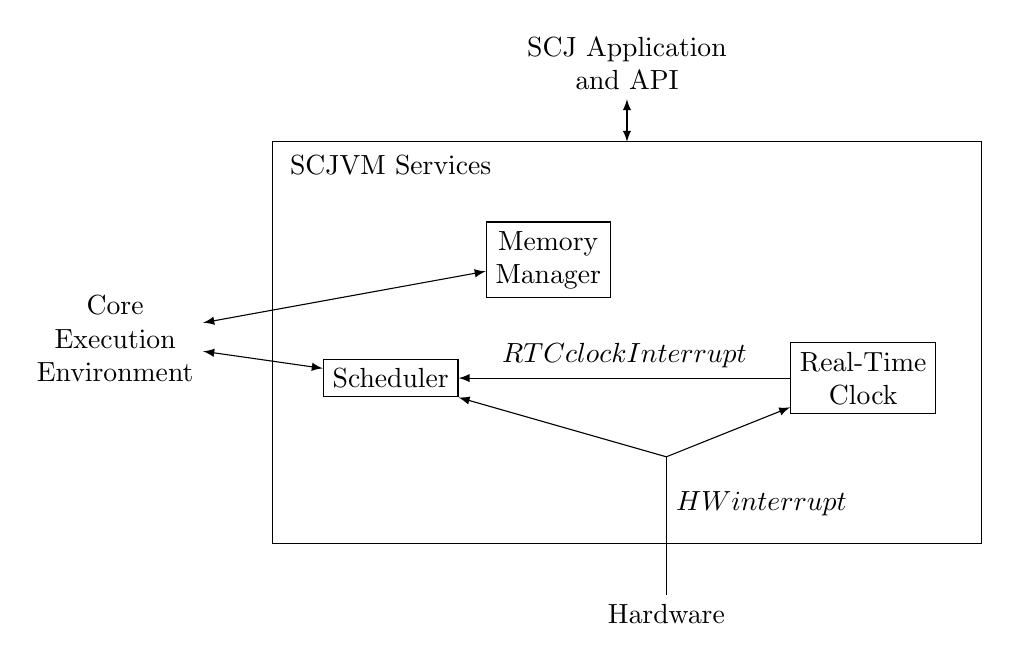
\begin{tikzpicture}
        \node[draw,align=center] (MM)  at (3.5cm,1.5cm) {Memory\\Manager};
        \node[draw,align=center] (S)   at (1.5cm,0cm)  {Scheduler};
        \node[draw,align=center] (RTC) at (7.5cm,0cm)  {Real-Time\\Clock};
        \draw (0cm,-2.1cm) rectangle (9cm,3cm);
        \node at (1.5cm,2.7cm) {SCJVM Services};
        
        \node[align=center] (HW) at (5cm,-3cm) {Hardware};
        
        \draw[-latex] (RTC) edge node[above] {$RTCclockInterrupt$} (S);
        
        \draw[-] (HW) -- node[above right] {$HWinterrupt$} coordinate[pos=1] (X) ++(0cm,2cm);
        \draw[-latex] (X) to (S);
        \draw[-latex] (X) to (RTC);
        
        \node[align=center] (CEE) at (-2cm,0.5cm) {Core\\Execution\\Environment};
        \draw[latex-latex] (S) -- (CEE);
        \draw[latex-latex] (MM) -- (CEE);
        
        \node[align=center] (App) at (4.5cm,4cm) {SCJ Application\\and API};
        \draw[latex-latex] (4.5cm,3cm) -- (App);
      \end{tikzpicture}
      \caption{The structure of the SCJVM services model, showing the
        channels used for communication between the processes in the
        model}
      \label{scjvm-services-model-fig}
\end{figure}

\chapter{The Core Execution Environment}
\label{cee-chapter}

This chapter describes the core execution environment (CEE) of an
SCJVM, which handles execution of an SCJ program.
% The CEE is aware of the structure of Java objects and classes in order
% to handle bytecode instructions properly.
In addition, the CEE of an SCJVM manages the flow of execution
dictated by the SCJ programming model, including, for example,
\texttt{Safelet} setup and mission execution.

This is the part of our SCJVM model that is handled by our compilation
strategy. 
So, it may take the form of a bytecode interpreter, which is the
starting point for the compilation, or C code, which is the output of
the compilation.
We describe both of these in this chapter
(Sections~\ref{cee-launcher-section}, \ref{cee-interpreter-section}
and~\ref{cee-c-code-section}) while the compilation strategy for
transforming between them is described in the next chapter.
We begin with an overview of the CEE's structure in the next section.
We conclude with some final considerations in
Section~\ref{cee-final-considerations-section}.

\section{Overview}

The CEE has three components, two of which depend on whether it is
interpreting bytecodes or executing C code. 
For the CEEs that use a bytecode interpreter, the components are
listed below and shown in Figure~\ref{cee-fig}:
\begin{itemize}
\item the object manager, which manages information about objects
  created during execution of the bytecode;
\item the interpreter itself, which handles execution of bytecode
  instructions; and
\item the launcher, which coordinates the startup of the SCJVM, the
  execution of missions, and the execution of methods in the
  interpreter.
\end{itemize}
% The interpreter is central to the main functionality of the core
% execution environment, but proper handling of infrastructure methods
% requires handling the SCJ mission-based programming model, which is
% dealt with by the launcher.
% The interpreter requires access to memory, but the class information
% and bytecode instructions do not change throughout the execution of
% the SCJVM, so they are provided as global constants in our model that
% are passed to the interpreter as parameters.
% Objects do change throughout the execution of the SCJVM and are in a
% separate region of memory to classes and bytecode instructions.
% The management of objects is handled by the object manager component
% of the core execution environment.

\begin{figure}[bth]
  \centering
  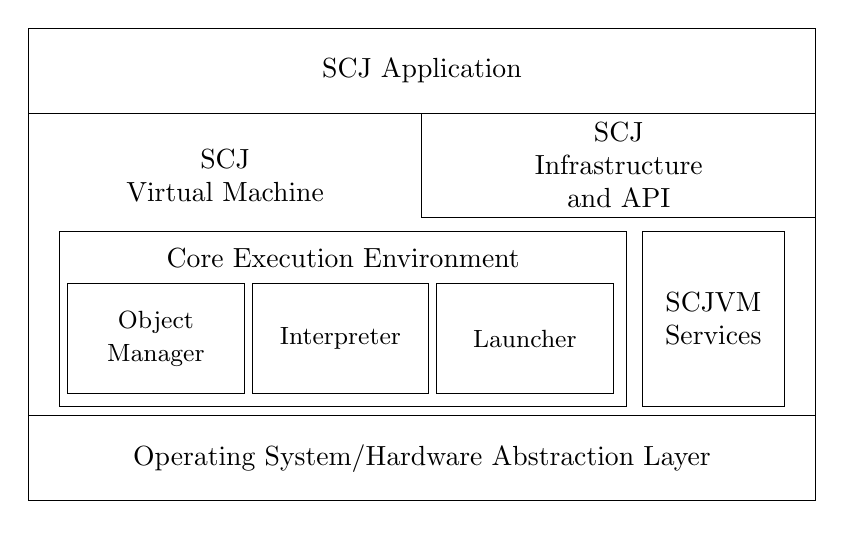
\begin{tikzpicture}

    \coordinate (width)  at (10cm,0cm);
    \coordinate (height) at (0cm,6cm);

    \path (0,0) -- (height)
    coordinate[pos=0.18] (OS boundary)
    coordinate[pos=0.20] (VM part bottom)
    coordinate[pos=0.57] (VM part top)
    coordinate[pos=0.60] (API boundary)
    coordinate[pos=0.82] (App boundary);
    
    \path (VM part bottom) -- (VM part top)
    coordinate[pos=0.7] (CEE part top);

    \path (VM part bottom) -- (VM part top)
    coordinate[pos=0.85] (CEE ypos);

    \path (0,0) -- (width)
    coordinate[pos=0.04] (CEE left)
    coordinate[pos=0.76] (CEE right)
    coordinate[pos=0.78] (VM Services left)
    coordinate[pos=0.96] (VM Services right)
    coordinate[pos=0.01] (CEE part sep);

    \path (CEE left) -- (CEE right)
    coordinate[pos=0.5] (CEE xpos);

    \path (0,0) to node[pos=0.5] (mid) {} (width);
    \path (0,0) to node[pos=0.25] (quart) {} (width);

    \draw (0,0) rectangle (width |- height);

    \draw (OS boundary) -- ++(width);
    \path (0,0) rectangle node[pos=0.5] (OS) {} (width |- OS boundary);
    \draw (mid |- API boundary) rectangle node[pos=0.5] (API) {} (width |- App boundary);
    \draw (App boundary) -- ++(width);
    \path (App boundary) rectangle node[pos=0.5] (App) {} (width |- height);

    \path (quart |- API boundary) rectangle node[pos=0.4] (SCJVM) {} (quart |- App boundary);
    \draw (CEE left |- VM part bottom) rectangle (CEE right |- VM part top);
    \draw (VM Services left |- VM part bottom) rectangle node[pos=0.5] (VM Services) {} (VM Services right |- VM part top);
    \coordinate (CEE) at (CEE xpos |- CEE ypos);

    \node[align=center] at (App)   {SCJ Application};
    \node[align=center] at (API)   {SCJ\\Infrastructure\\and API};
    \node[align=center] at (SCJVM) {SCJ\\Virtual Machine};
    \node[align=center] at (CEE)   {Core Execution Environment};
    \node[align=center] at (VM Services)  {SCJVM\\Services};
    \node[align=center] at (OS)    {Operating System/Hardware Abstraction Layer};

    \foreach \x in {1,...,3}
    \pgfmathsetmacro{\a}{0.33*(\x - 1)}
    \pgfmathsetmacro{\b}{0.33*\x}
    \path ($(CEE left) + (VM part bottom)!0.07!(VM part top)$) -- 
    node[pos=\a] (CEE part \x start) {}
    node[pos=\b] (CEE part \x end) {}
    ($(CEE right) + (VM part bottom)!0.07!(VM part top) - (CEE part sep)$);

    \foreach \x in {1,...,3} 
    \draw ($(CEE part \x start) + (CEE part sep)$)
    rectangle node[pos=0.5] (CEE part \x) {}
    (CEE part \x end |- CEE part top);
    
    \node[align=center] at (CEE part 1) {\small Object \\ \small Manager};
    \node[align=center] at (CEE part 2) {\small Interpreter};
    \node[align=center] at (CEE part 3) {\small Launcher};
  \end{tikzpicture}
  \caption{Structure of an SCJVM, showing the components of the CEE,
    and its relation to the SCJ infrastructure and the operating
    system/hardware abstraction layer}
  \label{cee-fig}
\end{figure}

The components after compilation to C are similar, but the object
manager is replaced with a struct manager, which manages C struct
types representing objects, and the interpreter is replaced with the C
program itself.
The launcher remains unchanged throughout the compilation.
It is assumed that it is already in the form of native code that can
be called from the C code.

The CEE is combined with the SCJVM services to form the complete
SCJVM; this is indicated in Figure~\ref{cee-fig}, which shows the same
structure described in Figure~\ref{scjvm-services-fig} in the previous
chapter, but has a focus on the CEE components.
The SCJVM services are unaffected by the compilation strategy and can
be implemented as a separate library.

Each of the components of the CEE is represented by a single \Circus{}
process in our model.
These processes interact as shown in Figure~\ref{cee-model-fig}.
The overall pattern of the interaction is unaffected by the
compilation, that is, the model of the compiled code has the same
overall flow of communication, although the components have different
names and different channels are used for communication.

\begin{figure}[ht]
  \centering
  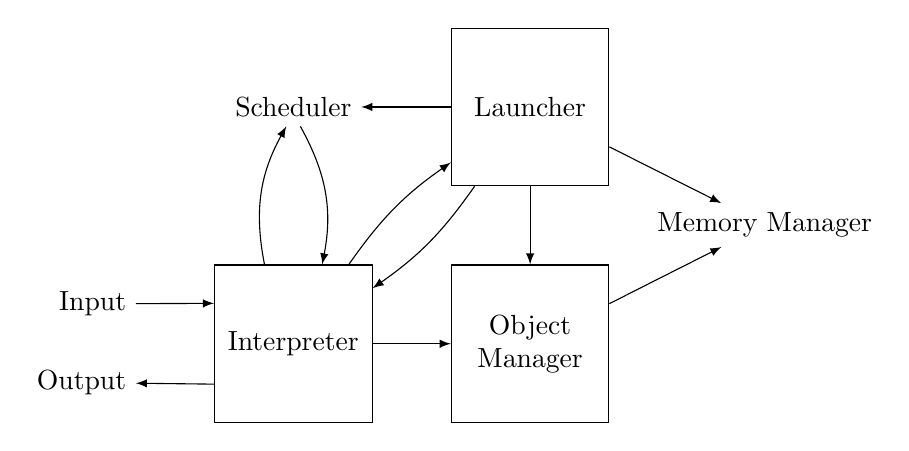
\begin{tikzpicture}
    \node[draw, minimum size=2cm, below right=2cm, align=center]
    (M) {Object\\Manager};
    \node[draw, minimum size=2cm, below=2cm]
    (I) {Interpreter};
    \node[draw, minimum size=2cm, right=2cm]
    (L) {Launcher};

    \draw[-latex, bend left=10] (I) edge (L);
    \draw[-latex, bend left=10] (L) edge (I);
    \draw[-latex] (I) edge (M);
    \draw[-latex] (L) edge (M);
    

    \node[below=1.5cm, right=4.5cm] (MM) {Memory Manager};
    \node[] (S) {Scheduler};
    \draw[-latex] (M) edge (MM);
    \draw (L) edge[-latex] (S);
    \draw (S) edge[-latex, bend left=20] (I);
    \draw (I) edge[-latex, bend left=20] (S);
    \draw (L) edge[-latex] (MM);

    \node[below=2.5cm, left=2cm] (In) {Input};
    \node[below=3.5cm, left=2cm] (Out) {Output};
    \draw[-latex] (In) to (I.153);
    \draw[-latex] (I.207) to (Out);
  \end{tikzpicture}
  \caption{The CEE model processes and their communication with each
    other and the SCJVM services}
  \label{cee-model-fig}
\end{figure}

The launcher manages the startup procedure for the SCJVM and the
execution of missions.
This involves communication with the interpreter (or C program) to
execute initialisation methods.
The interpreter then communicates back with the launcher when it
requires services that are provided by the SCJ infrastructure and API,
such as registering a schedulable object with the current mission.
Allocation of backing stores for the schedulable objects and entering
the corresponding memory areas involves communication with both the
object (or struct) manager in the CEE and the memory manager of the
SCJVM services.
The launcher must also communicate with the scheduler to indicate when
threads should be started or suspended during mission execution.

The interpreter must accept the requests to execute methods on the
main thread from the launcher, and it must also respond to requests
from the scheduler to start the other threads.
When a thread has finished execution, the interpreter signals to the
scheduler that the thread has finished so that it is no longer
scheduled.
The interpreter must also communicate with the launcher to handle
calls to methods that are provided by the SCJ infrastructure, such as
the methods to enter memory areas.
Handling of memory allocation during method execution is performed via
communication with the object manager, which then communicates with
the SCJVM memory manager.
Additionally, the interpreter communicates inputs and outputs to some
console input/output device, which is the only such device required by
the SCJ specification.
Supporting a full range of hardware connections is beyond the scope of
this work.

The interactions just described are modelled by channel
communications.
Those with the SCJVM services memory manager and scheduler use the
channels already described in
Sections~\ref{memory-manager-model-section}
and~\ref{scheduler-model-section}.
The types of values communicated by those channels are also used by
the CEE processes.
These include the type of object identifiers, $ObjectID$, the type of
thread identifiers, $ThreadID$, the type of backing store identifiers,
$BackingStoreID$, and the type of virtual machine data words, $Word$.
We also use the $ClassID$ and $MethodID$ types, which are the types of
class and method identifiers that are declared in the scheduler model
to permit the declaration of the $CEEstartThread$ channel.
Additionally, we declare a field identifier type, $FieldID$.
\begin{zed}
  [FieldID]
\end{zed}
The class, method and field identifiers may be the full names used in
Java class files or some shorter representation, such as unique
identification numbers.
In any case, type information needs to be taken into account so that
methods and fields with the same name, but different type signatures,
have different identifiers.
This is because the identifiers in Java class files include the type
information and the correct operation of method overloading relies on
it.

The channels used for communication between the CEE processes are
summarised in Figure~\ref{cee-channel-table}, with the full channel
declarations shown in Appendix~\ref{cee-model-channels}.
In addition to presenting the name and type for each channel, in the
first two columns of the table.
We also indicate which components of the CEE make use of the channel.
% L - launcher
% I - interpreter
% OM - object manager.
% I/L refers to a channel that is used by both the launcher and
% interpreter, with communications on that channel interleaved.
The channels $output$ and $input$ are used for communication with the
console device mentioned earlier.
As we do not model the console device itself, these are left as
externally visible channels when the component processes are composed
into the complete SCJVM model.
% The fact that they are external channels is indicated by the use of
% \textless{}ext.\textgreater{} in the final columns of the table.
Some channels are marked with various symbols (*, \dag{}, {}+{} and
\ddag{}) so that we can refer to them later in the text.

\begin{table}[t]
  \begin{center}
    \begin{tabular}{@{}lllll}
      \hline
      & Name & Parameter Type & \multicolumn{2}{l}{Communication} \\
      &      &                & from & to     \\
      \hline
      & $executeMethod$ & $ThreadID \cross ClassID \cross MethodID \cross \seq Word$ & L & I  \\
      & $executeMethodRet$ & $ThreadID \cross Word$ & I & L  \\
      & $continueExecution$ & $ThreadID$ & I & L \\
      & $initMainThread$ & $StackID$ & L & I \\ 
      *\dag & $register$ & $ThreadID \cross ObjectID$ & I & L \\
      %* & $registerRet$ & \textless no parameters\textgreater & L & I \\
      *\dag & $enterPrivateMemory$ & $ThreadID \cross \nat \cross ObjectID$ & I & L \\
      *\dag & $executeInAreaOf$ & $ThreadID \cross ObjectID \cross ObjectID$ & I & L \\
      *\dag & $executeInOuterArea$ & $ThreadID \cross ObjectID$ & I & L \\
      \dag & $enterPerReleaseMemory$ & $ThreadID \cross ObjectID$ & I & L \\
      {}+{} & $suspend$ & \textless no parameters\textgreater & I & L \\
      {}+{} & $suspendRet$ & \textless no parameters\textgreater & L & I \\
      {}+{} & $resumeThread$ & $ThreadID$ & I & L \\
      {}+{} & $resumeThreadRet$ & \textless no parameters\textgreater & L & I  \\
      & $output$ & $Word$ & I & \textless ext.\textgreater \\
      & $input$ & $Word$ & \textless{}ext.\textgreater{} & I \\
      & $enterBackingStore$ & $ThreadID \cross BackingStoreID$ & L & OM \\
      & $exitBackingStore$ & $ThreadID$ & L & OM  \\
      & $exitBackingStoreRet$ & $BackingStoreID \cross \boolean$ & L & OM \\
      & $getCurrentAC$ & $ThreadID$ & L & OM \\
      & $getCurrentACRet$ & $BackingStoreID$ & OM & L \\
      & $newObject$ & $ThreadID \cross ClassID$ & I/L & OM  \\
      & $newObjectRet$ & $ObjectID$ & OM & I/L  \\
      \ddag & $getClassIDOf$ & $ObjectID \cross ClassID$ & I/L & OM  \\
      \ddag & $getField$ & $ObjectID \cross FieldID$ & I & OM \\
      \ddag & $getFieldRet$ & $Word$ & OM & I \\
      \ddag & $putField$ & $ObjectID \cross FieldID \cross Word$ & I & OM \\
      \ddag & $getStatic$ & $ClassID \cross FieldID$ & I & OM \\
      \ddag & $getStaticRet$ & $Word$ & OM & I \\
      \ddag & $putStatic$ & $ClassID \cross FieldID \cross Word$ & I & OM \\
      & $addThreadMemory$ & $ThreadID \cross BackingStoreID$ & I & OM \\
      & $removeThreadMemory$ & $ThreadID$ & I & OM \\       
      \hline
    \end{tabular}
  \end{center}
  \caption{The channels used for communication between CEE processes
    before compilation. 
    In the final two columns, L refers to the launcher, I refers to
    the interpreter, OM refers to the object manager, I/L indicates a
    channel shared by the interpreter and launcher in interleaving,
    and \textless{}ext.\textgreater{} indicates and external channel.}
  \label{cee-channel-table}
\end{table}

Most of the channels are part of pairs, with one channel to
communicate a signal to begin an operation and supply any inputs, and
a return channel to communicate back when the operation has finished
and supply any outputs.
The return channel is named by appending $Ret$ to the name of the
channel used to initiate the operation.

There are some channels that deviate this pattern of having a return
channel.
The $executeMethod$ channel is used to signal to the interpreter that
it should begin execution of a method on a given thread.
The interpreter signals on $executeMethodRet$ channel when it has
finished execution of the method.
Since the launcher may need to take some action, such as exiting a
memory area, after the interpreter has finished executing a method,
the interpreter waits until it receives a signal on the
$continueExecution$ channel before continuing to execute.
Since the $continueExecution$ channel forms part of this communication
pattern, it does not have its own return channel.

Before the interpreter can execute methods on the $main$ thread, the
stack space for the $main$ thread must allocated by the launcher and
communicated to the interpreter.
This is handled by the $initMainThread$ channel, which carries the
$StackID$ for the stack space allocated for the $main$ thread.
The interpreter waits for communication on the $executeMethod$ channel
before commencing execution, so the launcher does not need to wait for
the interpreter to finish registering the $main$ thread's stack.

As mentioned above, while executing a method, the interpreter may
signal back to the launcher for handling of special methods.
The channels used for this are the ones marked with a * or a {}+{} in
Table~\ref{cee-channel-table}.
The channels marked with a * represent calls to infrastructure methods
that are part of the SCJ API.
The inputs and outputs of these methods (and hence the types of the
channels associated with them) are taken from the SCJ specification.
The channels marked with a \dag{} are methods that do not return a
value and involve execution of a method in the interpreter as part of
their handling.
Thus, the interpreter waits for a signal on the $executeMethod$
channel after signalling the launcher to handle one of these methods.
The methods marked with a \dag{} do not, therefore, require separate
return channels.
The channels marked with a + expose SCJVM scheduler operations to the
code executed in the interpreter, in order to allow for the
implementation of event handlers. 
Their types follow those of the scheduler's channels.

As mentioned previously, the $output$ and $input$ channels are used to
communicate $Word$ values to and from a console device.
The rest of the channels are used by the launcher and the interpreter
to communicate with the object manager.
The $enterBackingStore$ channel is used by the launcher to signal to
the object manager when a memory area is entered so that it can record
that the corresponding backing store has been entered.
This carries the $ThreadID$ of the thread to be entered, since the
backing stores entered are recorded separately for each thread, and
the $BackingStoreID$ of the backing store to be entered.
There is no corresponding return channel, since it is not necessary
for the launcher to wait while the object manager records the entry to
a backing store.
Similarly, the $exitBackingStore$ channel is used to signal an exit
from the backing store that is the current allocation context of the
given thread.
This does have a return channel, since the launcher must be informed
if the backing store was cleared due to no longer being in use by any
thread.
The $BackingStoreID$ of the exited backing store and a boolean value
indicating if the backing store was cleared are therefore communicated
back to the launcher on a return channel.
Additionally, the $getCurrentAC$ channel (and its return channel) is
used to obtain the $BackingStoreID$ of the backing store used as the
current allocation context for given thread from the object manager,
in order to handle some cases of entering memory areas.

The remaining channels used by the launcher to communicate with the
object manager are used by both the launcher and the interpreter.
These are the $newObject$ channel, which is used to allocate space for
new objects in the current allocation context, and the $getClassIDOf$
channel, which is used to obtain the $ClassID$ for the class of the
object associated with a given $ObjectID$.
% It is used for implementing the \texttt{new} bytecode in the
% interpreter and for creating infrastructure objects in the launcher.
% After compilation it represents a call to a method similar to
% \texttt{malloc()}.
The $newObject$ channel carries the $ThreadID$ of the current thread,
since there is a separate allocation context for each thread, and the
$ClassID$ of the class of the object to be allocated.
The object manager returns the $ObjectID$ of the newly allocated
object via the corresponding return channel.
The $getClassIDOf$ channel carries both the input and output to the
operation on the same channel, since it is a simple data accessing
operation that can be dealt with in a single communication.

The other channels used by the interpreter are the channels for
accessing fields of objects and classes.
The $getField$ channel is used for obtaining the value stored in a
given field of a given object.
It carries the $ObjectID$ of the object whose field is to be accessed
and the $FieldID$ of the field to be accessed.
The object manager then returns the $Word$ value stored in the field.
For putting a value into an object's field, the $putField$ channel is
used, which carries the $Word$ value to store in the field in addition
to the $ObjectID$ and $FieldID$ that identify the object and field to
update.
As this just updates the field and does not return any information,
there is no need for a return channel.
Channels for accessing static fields, $getStatic$ and $putStatic$, are
also provided.
These operate similarly to the channels for object fields but use
$ClassID$ values rather than $ObjectID$ values, since static fields are
attached to classes rather than objects.

The final channels used by the interpreter are the $addThreadMemory$
and $removeThreadMemory$ channels.
The $addThreadMemory$ is used to inform the object manager of a
thread's initial allocation context when the thread starts.
It carries the $ThreadID$ of the thread and the $BackingStoreID$ of
the backing store that serves as the thread's initial allocation
context.
When a thread has finished execution, it informs the object manager
via the $removeThreadMemory$ channel, which carries the $ThreadID$ of
the thread.

As mentioned earlier, some channels used by the interpreter to
communicate with the object manager are replaced with different
channels during compilation.
Those channels are marked with a \ddag{} in
Table~\ref{cee-channel-table}.
After compilation these channels are replaced with channels to obtain
the struct representing the contents of an object and to store an
object’s struct after updating it.
Note that the $getClassIDOf$ channel is shared between the launcher
and interpreter.
After compilation, the interpreter accesses a struct field storing the
$ClassID$ for an object.
However, the launcher is unaffected by the compilation and is agnostic
as to whether the program is in the form of bytecode or C code.
Therefore, the launcher continues to use the $getClassIDOf$ channel
after compilation, which represents a service offered by the object
manager or struct manager to obtain the $ClassID$ by whatever means
are appropriate to the form of the object.
As an optimisation in an implementation, the launcher could be changed
to access struct fields in the same way as the interpreter.
We discuss the form of field accesses in the C code and the channels
used for them in more detail in
Sections~\ref{cee-struct-manager-subsection}
and~\ref{cee-c-program-subsection}.

%\input{../../SCJ-VM/James/LIchans.zed}

%\input{../../SCJ-VM/James/memory_chans.zed}


Next, in Section~\ref{cee-launcher-section}, we describe our model of
the launcher.
We then detail the bytecode interpreter model in
Section~\ref{cee-interpreter-section}, and the C code model in
Section~\ref{cee-c-code-section}.

\section{Launcher}
\label{cee-launcher-section}

As mentioned in the previous section, the launcher is the component of
the CEE that manages the SCJVM startup and coordinates mission
execution.
It is described by the $Launcher$ process.

The launcher remains unaffected throughout the compilation strategy,
because it is agnostic to the class and bytecode information.
However, the launcher must know where to begin execution, so it takes
a parameter, $safeletClass$, which is the $ClassID$ of the
\texttt{Safelet} class.
This can be seen in the the $Launcher$ process definition, the
beginning of which is shown below.

Class initialisers must be executed as part of the SCJVM startup
procedure.
The order in which they are executed is determined by the dependencies
between class initialisers and classes, and is passed to the
$Launcher$ process as a second parameter, $initOrder$, which is a
sequence of $ClassID$s.
\begin{circus}
  \circprocess Launcher \circdef safeletClass : ClassID; initOrder : \seq ClassID \circspot \circbegin
\end{circus}

In what follows, we describe the definition of $Launcher$, focusing on
the aspects relevant for the compilation.
The complete definition can be found in
Appendix~\ref{launcher-appendix}.

The state of the $Launcher$ is divided into three parts.
The first part contains the identifiers of the objects that form the
SCJ mission model, so that the $Launcher$ can call methods of those
objects during SCJVM startup.
The second part contains information on the memory-area objects of
the program, including the relationship between the memory-areas and
the backing stores they represent, so that methods for entering and
exiting memory-areas can be handled.
The final part of the state describes the relationship between the
schedulable objects of SCJ and the threads used by the CEE so that the
threads can be started when mission execution begins.

We use separate Z schemas to specify each part of the state.
The first part is described by the $MissionManager$ schema, shown
below.
It contains the identifiers of three objects:
\begin{itemize}
\item $safelet$, the instance of the class implementing the
  \texttt{Safelet} interface for the program;
\item $missionSequencer$, the mission sequencer
  returned by the safelet's \texttt{getSequencer()} method; and
\item $currentMission$, the mission that is currently executing.
\end{itemize}
Methods of these objects are called at various points throughout SCJVM
startup and mission execution.
\begin{schema}{MissionManager}
  safelet, missionSequencer, currentMission : ObjectID
\end{schema}

The second part of the $Launcher$'s state is described by the
$MemoryAreaManager$ schema below.
It contains the identifiers of the memory-area objects for the
immortal memory, $immortalMemory$, and mission memory,
$missionMemory$.
There is a map, $backingStores$, that relates these identifiers and
the identifiers of the other memory-area objects, to the identifiers
of the backing stores they represent.
We also record the backing store identifiers of the per-release
memories for each thread in the $perReleaseMemories$ map.
Finally, to make sure that nested private memories can be reused,
there is a map from backing store identifiers to the identifiers of
private backing stores they contain, $privateMemoryMap$.
\begin{schema}{MemoryAreaManager}
  immortalMemory, missionMemory : ObjectID \\
  backingStores : ObjectID \finj BackingStoreID \\
  perReleaseMemories : ThreadID \finj BackingStoreID \\
  privateMemoryMap : BackingStoreID \finj BackingStoreID
\where
  \cdots
\end{schema}
Each of the maps in the $MemoryAreaManager$ is injective, since each
memory-area object has a distinct backing store and memory-areas
cannot share a nested private memory-area.
The invariants of $MemoryAreaManager$ are elided above. 
They ensure that each memory-area object has a corresponding backing
store in $backingStores$, and that areas which are not nested private
memories do not appear in the range of $privateMemoryMap$.

The final part of the state is specified in the $SchedulableManager$
schema below.
It contains a map, $schedulableThreads$, from the identifiers of
schedulable objects to the identifiers of the threads associated with
them.
This map must be injective, since every schedulable object has a
separate thread.
\begin{schema}{SchedulableManager}
  schedulableThreads : ObjectID \finj ThreadID
\end{schema}

The state of the process is then the conjunction of these three
schemas.
\begin{circusaction}
  \circstate LauncherState == MissionManager \land MemoryAreaManager \land SchedulableManager
\end{circusaction}

The $Launcher$ state is initialised as described in $LauncherInit$,
which is shown below.
The object identifiers are initialised to the $null$ identifier.
They are later filled with non-$null$ identifiers as the corresponding
objects are created during SCJVM execution.
Similarly, each of the maps is initialised to the empty set.
\begin{schema}{LauncherInit}
	LauncherState~'
\where
	\{ safelet', missionSequencer', currentMission', immortalMemory', missionMemory' \} \\
	\t1 {} \subseteq \{ null \} \\
	backingStores' = \emptyset \\
	perReleaseMemories' = \emptyset \\
	privateMemoryMap' = \emptyset \\
	schedulableThreads' = \emptyset
\end{schema}

The main action of the $Interpreter$ proceeds as shown below.
The state is first initialised as described by $LauncherInit$ and then
the actions $Startup$ and $RunNextMission$ follow in sequence.
$Startup$ defines the SCJVM startup procedure that must be performed
once at the start of SCJVM execution, whereas $RunNextMission$ defines
the procedure that must be performed for each mission run.
We do not handle mission termination in our $Launcher$ model.
This is because the SCJ mission termination procedure has almost no
effect on our compilation strategy; a single mission is sufficient for
our examples to evaluate the compilation strategy.
A formal account of it is available elsewhere~\cite{cavalcanti2013,
  luckcuck2016, zeyda2011}. 
Thus, $RunNextMission$ is only executed once.
\begin{circusaction}
  \circspot \lschexpract LauncherInit \rschexpract \circseq Startup \circseq RunNextMission
\end{circusaction}

The definition of $Startup$ is shown below.
It performs a number of actions in sequence, following the startup procedure for an SCJVM:
\begin{itemize}
\item creating the main thread's stack and passing on the
  $initMainThread$ channel, in $MakeMainStack$;
\item executing the class initialisers in the order given in
  $initOrder$, in $RunClassInitialisers$;
\item creating the immortal memory object that corresponds to the root
  backing store and storing it in $immortalMemory$, in
  $CreateImmortalMemory$;
\item creating the \texttt{Safelet} object and storing it in
  $safelet$, in $CreateSafelet$;
\item calling the \texttt{immortalMemorySize()} and
  \texttt{globalBackingStoreSize()} methods of the $safelet$, and
  checking that the size of the root backing store matches those
  values, in $CheckImmortalMemory$ and $CheckRemainingBackingStore$;
\item calling the \texttt{initializeApplication()} method of the $safelet$, in $InitializeApplication$;
\item calling the $safelet$'s \texttt{getSequencer()} method and
  storing the returned value in $missionSequencer$, in $GetSequencer$;
  and
\item creating the $missionMemory$ object with its corresponding backing store, in $CreateMissionMemory$.
\end{itemize}
\begin{circusaction}
  Startup \circdef MakeMainStack \circseq RunClassInitialisers \circseq CreateImmortalMemory \circseq CreateSafelet \circseq \\
  \t1 CheckImmortalMemory \circseq CheckRemainingBackingStore \circseq InitializeApplication \circseq \\
  \t1 GetSequencer \circseq CreateMissionMemory
\end{circusaction}

$RunNextMission$ begins with calling the \texttt{getNextMission()}
method of $missionSequencer$, in the action $GetNextMission$.
The returned mission is stored in $currentMission$.
Its \texttt{missionMemorySize()} method is then executed, and the
backing store of $missionMemory$ is resized to match, in
$ResizeMissionMemory$.
Next, in $InitializeMission$, the mission's \texttt{initialize()}
method is executed, during which the schedulable objects for the
mission are registered.
Afterwards, in $InitialiseAndStartThreads$, the registered schedulable
objects have their stacks and backing stores created, after which the
threads for all the schedulable objects are started.
Finally, in $WaitForExecution$, the $main$ thread suspends itself and
the $Launcher$ then waits, handling special methods for the threads of
the program when necessary.
Since termination is not handled, this phase of the program continues
indefinitely.
\begin{circusaction}
  RunNextMission \circdef GetNextMission \circseq ResizeMissionMemory \circseq InitializeMission \circseq \\
  \t1 InitialiseAndStartThreads \circseq WaitForExecution
\end{circusaction}

During these actions, methods are executed using the channels
$executeMethod$, $executeMethodRet$ and $continueExecution$, discussed
earlier.
The identifiers of the methods, which may be standard methods from the
SCJ API, or implementation-defined API methods required by the
launcher, are represented by constants in the model.
Although most of the methods used by the $Launcher$ are executed
simply by communicating on each of the channels mentioned above in
turn, as noted above, in $InitializeMission$, the
\texttt{initialize()} method of a mission requires handling of the
\texttt{register()} method for each schedulable object.
We must also provide handling for other special methods.
This is done in the $HandleSpecialMethodsMainLoop$ action below, which
offers handling of the special methods while waiting for return from
the \texttt{initialize()} method on the $executeMethodRet$ channel.
A similar action, without the final choice accepting
$executeMethodRet$, is used to handle special methods in
$WaitForExecution$.
\begin{circusaction}
  HandleSpecialMethodsMainLoop \circdef \circval memoryEntries : ThreadID \fun \nat; \circres retVal : Word \circspot \\
  \t1 (\Extchoice t : ThreadID \circspot \\
  \t2 EnterMemory(t) \circseq \\
  \t2 HandleSpecialMethodsMainLoop(memoryEntries \oplus \{ t \mapsto memoryEntries~t + 1 \}, retVal)) \\
  \t1 {} \extchoice {} \\
  \t1 (\Extchoice t : ThreadID \circspot \\
  \t2 \lcircguard memoryEntries~t > 0 \rcircguard \circguard ExitMemory(t) \circseq \\
  \t2 HandleSpecialMethodsMainLoop(memoryEntries \oplus \{ t \mapsto memoryEntries~t - 1 \}, retVal)) \\
  \t1 {} \extchoice {} \\
  \t1 ((Register \extchoice Suspend \extchoice Resume) \circseq \\
  \t2 HandleSpecialMethodsMainLoop(memoryEntries, retVal)) \\
  \t1 {} \extchoice {} \\
  \t1 (\lcircguard \forall t : ThreadID @ memoryEntries~t = 0 \rcircguard \circguard {} \\
  \t2 executeMethodRet?thr \prefixcolon (thr = main) ?r \then continueExecution!main \then retVal := r)
\end{circusaction}
$HandleSpecialMethodsMainLoop$ takes a value parameter,
$memoryEntries$, which is a map recording how many times a memory area
has been entered for each thread.
It also take a value parameter, $retVal$, which captures the return
value from the execution of the method on the $main$ thread.
It offers a choice of handling a memory-area entry, handling the
corresponding memory-area exit, handling a special method that does
not enter memory-areas, or accepting return from the execution of the
method on the $main$ thread (handled in the usual way using
$executeMethodRet$ and $continueExecution$, with the return value
stored in $retVal$).

$HandleSpecialMethodsMainLoop$ handles memory-area entering
methods, which execute another method after entering a memory-area,
during which further special methods may be called.
Each entry to a memory-area must be matched by a corresponding exit
from the memory-area when this extra method execution returns.
Thus, the entries to memory-areas are tracked in the $memoryEntries$
map.

The number stored in $memoryEntries$ for a thread identifier $t$ is
incremented after handling a memory-area entry on that thread as
described in $EnterMemory(t)$.
Similarly, it is decremented after handling exit from the memory-area
in $ExitMemory(t)$, which is only offered if the value is already
greater than zero.
After handling memory-area entry or exit, or another special method
(handled in the actions $Register$, $Suspend$ and $Resume$),
$HandleSpecialMethodsMainLoop$ recurses to allow further special
methods to be handled.
The return from the top-level method execution on the $main$ thread is
only permitted once all memory areas have been exited and
$memoryEntries$ is zero for all threads.

To illustrate how the nested method execution after memory-area entry
is performed, we show the $ExecuteInAreaOf$ action below, which is one
of the actions offered in external choice in $EnterMemory$, along with
actions to handle other memory-area entering operations.
$ExecuteInAreaOf$ takes a thread identifier $thread$ as a parameter
and only accepts communications from that thread, so that we can
separate out memory-area entries for each thread.
The identifier of a \texttt{Runnable} object, $runnable$, is received
via the $executeInAreaOf$ channel, which is the object that indicates
the method to be executed in the memory-area. 
Such an identifier is received for all of the memory-area entering
methods.
In the case of $ExecuteInAreaOf$, another identifier, $object$, is
also received and a $FindBackingStore$ action is used to communicate
with the memory manager to determine its backing store.
This backing store is then entered, via communication on the
$enterBackingStore$ channel.
The class of the $runnable$ object is determined and its
\texttt{run()} method (represented here by the $run$ identifier) is
executed by signalling on the $executeMethod$ channel.
No communication on the $executeMethodRet$ channel is waited for in
this action, because it is handled separately in the $ExitMemory$
action since other special methods (including further memory entries)
may occur inbetween.
\begin{circusaction}
  ExecuteInAreaOf \circdef \\
  \t1 \circval thread : ThreadID \circspot \circvar runnable, object : ObjectID; bs : BackingStoreID \circspot \\
  \t1 executeInAreaOf?t \prefixcolon (t = thread) ?obj?r \then object, runnable := obj, r \circseq \\
  \t1 FindBackingStore(object, bs) \circseq \\
  \t1 enterBackingStore!thread!bs \then getClassIDOf!runnable?runnableClass \\
  \t1 {} \then executeMethod!thread!runnableClass!run!(\langle runnable \rangle) \then \Skip
\end{circusaction}
The return from the \texttt{run()} method, and the exit from the
memory-area, is specified by the $ExitMemory$ action below.
This, as with the $ExecuteInAreaOf$ action, takes a $thread$
parameter.
A return from a method executing on that thread is accepted on the
$executeMethodRet$ channel, and its return value is discarded as the
\texttt{run()} method is \texttt{void}.
The exit from the memory-area is then performed using the
$exitBackingStore$ and $exitBackingStoreRet$ channels.
The $Launcher$ state may afterwards be updated to account for the
exited memory-area being cleared (due to no longer being in use by any
thread), which is specified in the $ClearPrivateMemory$ schema.
After the exit from the memory-area has been handled, the $Launcher$
signals that normal execution on $thread$ may continue using the
$continueExecution$ channel.
\begin{circusaction}
  ExitMemory \circdef \circval thread : ThreadID \circspot \\
  \t1 executeMethodRet?t \prefixcolon (t = thread) ?void \\
  \t1 {} \then exitBackingStore!thread \then exitBackingStoreRet?bsid?isCleared \then {} \\
  \t1 \circif isCleared = \true \circthen \lschexpract ClearPrivateMemory[bsid/toClear?] \rschexpract \\
  \t1 {} \circelse isCleared = \false \circthen \Skip \\
  \t1 \circfi \circseq continueExecution!thread \then \Skip
\end{circusaction}

The \texttt{register()} method also needs to execute a method in the
interpreter to obtain a thread's priority.
Further special methods are not handled in this case, since the method
to obtain a thread's priority is expected to be a simple method that
does not call special methods.

This handling of special methods is used by the interpreter process
(or C program, after compilation), which must communicate with the
$Launcher$ when such methods are encountered.
To allow for the behaviour of executing methods after entering memory
areas (or during the \texttt{register()} method), the interpreter must
also be prepared to execute another method after signalling to the
$Launcher$.
This is transformed to nested method executions during the compilation
strategy in order to preserve the communication pattern with the
$Launcher$.
We describe in more detail how this communication is performed in the
interpreter in Section~\ref{cee-interpreter-subsection}, and in C
program in Section~\ref{cee-c-program-subsection}.
In the next section, we describe the bytecode interpreter, which,
along with the $Launcher$, forms the CEE before the application of the
compilation strategy.

% \input{../../SCJ-VM/James/launcher.zed}

\section{Bytecode Interpreter Model}
\label{cee-interpreter-section}

This section describes the bytecode interpreter that handles execution
of an SCJ bytecode program.
Its model is composed of two processes:~the model of the object
manager, $ObjMan$, and the model of the interpreter itself,
$Interpreter$.
These are composed together in parallel with the $Launcher$ to form
the complete core execution environment, $CEE$, as shown below.
The synchronisation sets and channel hidings, omitted here, are
consistent with the communication patterns shown in
Table~\ref{cee-channel-table}.
The parameters of each of the components, including the classes, $cs$,
and bytecode instructions, $bc$, which are explained later in this
section, become parameters of $CEE$.
\begin{circus}
  CEE(cs,bc,sid,initOrder) \circdef ObjMan(cs) \parallel
  Interpreter(cs,bc) \parallel Launcher(sid,initOrder)
\end{circus}

In Section~\ref{cee-bytecode-subset-subsection}, we first give an
informal description of the bytecode instructions handled in our model
and the ways in which their SCJ semantics differ from that of standard
Java.
In Section~\ref{cee-classes-subsection}, we describe our model of Java
class information that is used by both $ObjMan$ and $Interpreter$.
The first component, $ObjMan$, is described in
Section~\ref{cee-object-manager-subsection} and the second,
$Interpreter$, in Section~\ref{cee-interpreter-subsection}.

\subsection{Bytecode Subset}
\label{cee-bytecode-subset-subsection}

We model a subset of Java bytecode sufficient to express a wide
variety of SCJ programs and illustrate how further features may be
added, but small enough to permit effective reasoning.
The subset has been chosen by considering the bytecode generated from
a simple SCJ program and removing instructions similar to those
already in the subset.
This ensures the model is not unnecessarily complicated with trivial
or redundant instructions, so we can concentrate on the instructions
that are most of interest in creating the compilation strategy.
The bytecode instructions in our subset are described in
Table~\ref{bytecode-subset-table}.

\begin{table}
  \centering
  \begin{tabular}{llp{8.5cm}}
    \hline
    Instruction & Parameter & Description \\
    \hline
    \texttt{aconst\_null} & (none) & 
    Pushes a null object reference onto the operand stack.
    \\
    \texttt{aload} & local variable index &
    Loads the value from a specified local variable and pushes it
    onto the operand stack.
    \\
    \texttt{areturn} & (none) &
    Returns from the current method, pushing the value on top of the
    current method's operand stack onto the operand stack of the
    method returned to.
    \\
    \texttt{astore} & local variable index &
    Pops a value from the operand stack and stores it in the specified
    local variable.
    \\
    \texttt{dup} & (none) &
    Duplicates the value on top of the operand stack.
    \\
    \texttt{getfield} & constant pool index &
    Pops an object reference from the operand stack, gets the value of
    the field specified by the identifier at the given constant pool
    index for the referenced object, and pushes it onto the operand
    stack.
    \\
    \texttt{getstatic} & constant pool index &
    Gets the value of the static field specified by the field and
    class identifiers at the given constant pool index, and pushes it
    onto the operand stack.
    \\
    \texttt{goto} & program address &
    Unconditionally branches to the given program address.
    \\
    \texttt{iadd} & (none) &
    Pops two integer values from the operand stack, adds them, and
    pushes the result onto the operand stack.
    \\
    \texttt{iconst} & integer value &
    Pushes the given integer value onto the operand stack of the
    current method.
    \\
    \texttt{if\_icmple} & program address &
    Pops two integer values from the operand stack, and branches to
    the given program address if the second value popped is less than
    or equal to the first value.
    \\
    \texttt{ineg} & (none) &
    Pops an integer value from the operand stack, negates it, and
    pushes the negated value onto the operand stack.
    \\
    \texttt{invokespecial} & constant pool index &
    Gets the method and class identifier at the given constant pool
    index and invokes the specified method of the specified class,
    popping the method's arguments, plus a \texttt{this} object
    reference, from the operand stack.
    \\
    \texttt{invokestatic} & constant pool index &
    Gets the method and class identifier at the given constant pool
    index and invokes the specified method of the specified class,
    popping the method's arguments from the operand stack.
    \\
    \texttt{invokevirtual} & constant pool index &
    Gets the method and class identifier at the given constant pool
    index, pops the arguments of the specified method, including a
    \texttt{this} object reference, from the operand stack, and
    invokes the specified method of the class of referenced object.
    \\
    \texttt{new} & constant pool index &
    Allocates a new object of the class specified by the identifier at
    the given constant pool index and pushes a reference to the new
    object onto the operand stack.
    \\
    \texttt{putfield} & constant pool index &
    Pops an object reference and value from the operand stack and
    stores the value in the field specified by the identifier at the
    given constant pool index for the referenced object.
    \\
    \texttt{putstatic} & constant pool index &
    Pops a value from the operand stack and stores the value in the
    static field specified by the field and class identifiers at the
    given constant pool index.
    \\
    \texttt{return} & (none) &
    Returns from a method with no return value.
    \\
    \hline
  \end{tabular}
  \caption{The instructions in our bytecode subset}
  \label{bytecode-subset-table}
\end{table}

Java bytecode instructions operate over a state that records
information on all loaded classes, a stack frame, and the object data
residing in memory.
Various pieces of class information are required for execution of
bytecode instructions, but a constant pool, which stores all the
constants and names required by the class, is the main information
used.

The constant pool contains references to classes, methods and fields
used by the bytecode instructions in the class, as well as constant
values used in the code.
The form of the constant pool is a large array.
Indices into this array are used as parameters to instructions
requiring information from the constant pool.
For example, the \texttt{getfield} and \texttt{putfield} instructions
take constant pool index parameters pointing to a reference to a field
whose value should be obtained or set.
Other class information used at runtime includes information on fields
and methods belonging to the class, which is required for creation of
objects and invocation of methods.

The frame stack forms the second part of the JVM manipulated by
bytecode instructions and consists of a series of frames that contain
the runtime information for each invocation of a method.
When a method is invoked, a new stack frame is created for it and
pushed onto the frame stack, and when the method returns, the stack
frame is popped from the stack.

Each stack frame contains an operand stack, which is used to store
values manipulated by bytecode instructions, and an array of local
variables.
Most bytecode instructions manipulate the operand stack in some way,
popping arguments from it, pushing results to it or performing
specific operations upon it.

The local variables are used to store the arguments of a method and
the results of computations performed on the operand stack.
Operations are not performed directly on the local variables, so the
only bytecode instructions that affect them are those for moving
values between the operand stack and the local variables
(\texttt{aload} and \texttt{astore} are examples of such
instructions).

Some bytecode instructions also manipulate objects, which in our case
reside in backing store memory.
Such instructions include \texttt{new}, which creates objects, and
\texttt{getfield}, which gets the value from a field of an object.
In our choice of instructions for the subset, we mainly focus on
manipulation of objects and method invocation, since those are core
concepts of Java bytecode and require special handling by the
compilation strategy.

The instruction \texttt{dup} is included as an example of a simple
instruction that operates on the operand stack.
It has been chosen for its frequent occurrence in object initialisation.
Other instructions that do simple operand stack manipulation,
including the arithmetic instructions, can be specified similarly.

We also include a few arithmetic instructions as an example of how
integers are handled.
Specifically, we include the integer addition operation,
\texttt{iadd}, as an example of a binary operation, and the integer
negation operation, \texttt{ineg}, as an example of an unary
operation.
We do not include operations for floating point values since the
operations upon them are not substantially different from those on
integers at the level of modelling and compilation.
The model can be easily extended to include more integer operations.

Instructions that create object references (the \texttt{new} and
\texttt{aconst\_null} instructions), pass them around (\texttt{aload},
\texttt{astore}, \texttt{areturn}, etc.), and permit
field accesses (\texttt{getfield} and \texttt{putfield}) are also
included to allow the full range of object manipulations.
We also provide instructions for \texttt{static} field accesses
(\texttt{getstatic} and \texttt{putstatic}) since they are of use in
sharing data between different parts of the program.
However, arrays are not included as they require additional
instructions and can be emulated, albeit inefficiently, with the
instructions given here.

Both the \texttt{invokevirtual} and \texttt{invokespecial}
instructions, which invoke methods on objects, are included.
The \texttt{invokevirtual} instruction looks up the method to invoke
in the method table for the class of the object that the method is
invoked on.
The \texttt{invokespecial} instruction, on the other hand, uses the
class identifier supplied in the method reference pointed to by the
parameter of the instruction when looking up the method.
The \texttt{invokestatic} instruction, for invoking \texttt{static}
methods of classes, is similar to \texttt{invokespecial}, but does not
supply a \texttt{this} object parameter, whereas
\texttt{invokevirtual} and \texttt{invokespecial} pop \texttt{this}
from the stack as an extra argument.

The \texttt{goto} and \texttt{if\_icmple} instructions are provided as
examples of control flow instructions, with \texttt{goto} representing
an unconditional branch and \texttt{if\_icmple} representing a
conditional branch.
Other forms of conditional branch may be implemented in a similar
fashion to \texttt{if\_icmple}, but we do not include those in our
subset since \texttt{if\_icmple} is sufficient to represent most
control flow structures.
Although \texttt{goto} could be represented as a special case of
\texttt{if\_icmple}, we include it as a separate instruction due to
its frequent use in conjunction with \texttt{if\_icmple} to implement
loops.

We do not handle exceptions; errors in the SCJVM are instead handled
by simply aborting execution.
SCJ programs can be statically verified to prove that exceptions will
not be thrown~\cite{kalibera2010,marriott2014}.
Furthermore, reliance on exceptions to handle errors has been
discouraged by an empirical study due to the potential for errors in
exception handling~\cite{sawadpong2012}.
The bytecode instructions that relate to throwing and catching
exceptions are, therefore, not included in our bytecode subset.

As a simplifying assumption, we consider that all values consist of
only a single virtual machine word.
This means that \texttt{long} and \texttt{double} values are not
handled.
Any SCJ API methods that take \texttt{long} or \texttt{double}
arguments are viewed as taking \texttt{int} or \texttt{float} instead.
The reason for this assumption is that handling of two word values
makes little difference at the level of the formal model and our
approach can be easily extended to deal with more types.

Further, we do not make a distinction between the different virtual
machine types in our bytecode instructions.
This is justified as the bytecode instructions simply handle values as
32-bit words, with the type information only used for typechecking
during bytecode validation. 
The code passed into the core execution environment is assumed to have
already passed, which may be done by a separate
component~\cite{klein2003, stark2001, coglio2000, xavier2003}). 
Since many of the instructions behave the same for different types, we
only include those instructions that handle values as object
references.
We would introduce a lot of duplication in the model if, for example,
both the \texttt{areturn} and \texttt{ireturn} instructions were to be
included.

Because we are considering bytecode arising from an SCJ program, some
requirements of SCJ permit further simplifications to our bytecode
subset.
The \texttt{invokedynamic} instruction performs method invocation with
runtime typechecking, mainly for the purpose of implementing
dynamically-typed languages targeting the JVM (though it is also used
to implement the lambda expressions introduced in Java 8).
It is not included in our subset as it does not allow static
typechecking and so should not be used for SCJ.

The requirement for all classes to be loaded at startup greatly
simplifies the semantics of several instructions, since dynamic class
loading does not need to be considered.
It also means that method lookup tables can be precomputed.
This means that the semantics of the \texttt{invokevirtual} and
\texttt{invokeinterface} instructions are the same, since they both
invoke a method on an object, using the object's class as the class
for method lookup.
They, therefore, do not both need to be included and so we have not
included the \texttt{invokeinterface} instruction, since it exists
only to optimise method lookup.

In terms of concurrency considerations, we are assuming our SCJVM to
be single processor, and so we do not need to have more than one
interpreter.
As we see later, the interpreter's threads are modelled using separate
\Circus{} processes, but execution only occurs on one at a time.
We also assume that thread switches can only occur between bytecode
instructions in the interpreter.
This is justified since bytecode instructions should appear to be
atomic.
An implementation may be non-atomic as long as the externally visible
sequence of events is the same as for the model with atomic
instructions.
This means that instructions requiring communication with other
components of the SCJVM, such as \texttt{new}, which communicates with
the memory manager, must be atomic since that they affect shared
state.

Having described our bytecode subset and the assumptions we are
making, we now proceed to describe our model of Java classes in the
next section.

\subsection{Classes}
\label{cee-classes-subsection}

In our model, information about the Java classes that form the program
is recorded in a map, $cs$, that is provided as a parameter to $CEE$.
The $cs$ map associates $ClassID$s with records of a schema type
$Class$ defined as the conjunction of three schemas.
The first schema, $ClassConstantPool$ contains components that
represent the constant pool and indices into the constant pool.
The second schema, $ClassMethods$, represents information on the
methods in the class.
The final schema, $ClassFields$, is our model for information on the
fields in the class.

The components of $ClassConstantPool$ are $constantPool$, the constant
pool itself, and some indices into $constantPool$:~$this$, referencing
the current class, $super$, referencing the current class' superclass,
and $interfaces$, a set of indices referencing the interfaces
implemented by the current class.
\begin{schema}{ClassConstantPool}
  constantPool : CPIndex \pfun CPEntry \\
  this, super : CPIndex \\
  interfaces : \finset CPIndex
\where
  % the null constant pool entry is not a valid constant pool entry
  nullCPIndex \notin \dom constantPool \\
  % this, super and interfaces must all be valid constant pool indicies (except that super may be null)
  \{this\} \cup (\{ super\} \setminus \{nullCPIndex\}) \cup interfaces \subseteq \dom constantPool \\
  % this, super and interfaces must point to ClassRefs
  constantPool \limg \{this, super\} \cup interfaces \rimg \subseteq \ran ClassRef
\end{schema}
% \begin{schema}{Class}
%   constantPool : CPIndex \pfun CPEntry \\
%   this, super : CPIndex \\
%   interfaces : \finset CPIndex \\
%   methodEntry, methodEnd : MethodID \pfun ProgramAddress \\
%   methodLocals, methodStackSize : MethodID \pfun \nat \\
%   fields, staticFields : \finset FieldID
% \where
%   % the null constant pool entry is not a valid constant pool entry
%   nullCPIndex \notin \dom constantPool \\
%   % this, super and interfaces must all be valid constant pool indicies (except that super may be null)
%   \{this\} \cup (\{ super\} \setminus \{nullCPIndex\}) \cup interfaces \subseteq \dom constantPool \\
%   % this, super and interfaces must point to ClassRefs
%   constantPool \limg \{this, super\} \cup interfaces \rimg \subseteq \ran ClassRef \\
%   \dom methodEntry = \dom methodEnd = \dom methodLocals = \dom methodStackSize \\
%   \forall m : \dom methodEntry @ methodEntry~m \leq methodEnd~m \\
%   % a method's local variables must at least include space for its arguments
%   \forall m : \dom methodLocals @ methodArguments~m \leq methodLocals~m
% \end{schema}
The entries of $constantPool$ are indexed by a elements of a type
$CPIndex$.
In the JVM, the $CPIndex$ values are positive integers, but no
arithmetic or comparison is performed on constant pool indices in our
model, so we do not represent that fact.

We distinguish one particular $CPIndex$ value, a constant
$nullCPIndex$, which represents an invalid index into the
$constantPool$.
It is used as a placeholder in cases when no index is present.
For example, the class \texttt{Object} has no superclass, so the index
of the constant pool entry referencing its superclass is
$nullCPIndex$.

Each of the entries in the $constantPool$ is represented by an element
of a free type $CPEntry$, the definition of which is shown below.
It has three constructors:~$ClassRef$, representing a reference to a
$ClassID$, $MethodRef$, representing a reference to a method of a
particular class by a $ClassID$ and $MethodID$, and $FieldRef$,
representing a reference to a field of a particular class by a
$ClassID$ and $FieldID$.
\begin{zed}
  CPEntry ::= \\
  \t1 ClassRef \ldata ClassID \rdata | MethodRef \ldata
  ClassID \cross MethodID \rdata | FieldRef \ldata ClassID \cross
  FieldID \rdata
\end{zed}
Although there are other types of constant pool entry described in the
JVM specification, we do not include them in our model since some of
them are not relevant to our subset. 
Some constant pool entries are used by other constant pool entries.
For example, in the JVM specification, method references reference
another constant pool entry, which in turn contains references to
further constant pool entries with string representations of the
method's name and type.
In our model, we hide this complexity in the identifier types
$ClassID$, $MethodID$ and $FieldID$, omitting the extra constant pool
entries.

The first conjunct of the invariant of $ClassConstantPool$ requires
that $nullCPIndex$ not be in the domain of $constantPool$, since
$nullCPIndex$ is not a valid index into $constantPool$.
The second conjunct states that the indices $this$, $super$, and
$interfaces$ must be in the domain of $constantPool$, unless $super$
is $nullCPIndex$ (which is the case for the \texttt{Object} class).
Finally, the third conjunct requires that the $constantPool$ entries
at $this$, $super$ and $interfaces$ are $ClassRef$s.

The components of $ClassMethods$, shown below, are maps from
$MethodID$ values to information about each method.
The first two, $methodEntry$ and $methodEnd$, map to $ProgramAddress$
values, which are indices into a separate bytecode array representing
the start and end points of the method.
The last two components, $methodLocals$ and $methodStackSize$, map to
natural numbers giving the required number of local variables and
operand stack slots for the method.
These values are used during the compilation strategy to declare C
variables to store the local variables and operand stack values.
\begin{schema}{ClassMethods}
  methodEntry, methodEnd : MethodID \pfun ProgramAddress \\
  methodLocals, methodStackSize : MethodID \pfun \nat
\where
  \dom methodEntry = \dom methodEnd = \dom methodLocals = \dom methodStackSize \\
  \forall m : \dom methodEntry @ methodEntry~m \leq methodEnd~m \\
  % a method's local variables must at least include space for its arguments
  \forall m : \dom methodLocals @ methodArguments~m \leq methodLocals~m
\end{schema}
In addition to the components of $ClassMethods$, we declare a global
function $methodArguments$ from $MethodID$s to natural numbers, which
gives the number of arguments that each method takes.
This is a global function since each $MethodID$ encodes the type of
the method, so the number of arguments for a method can always be
determined from its identifier.
The $methodArguments$ function is also total for this reason.
We use $methodArguments$ in the invariant of $ClassMethods$, and also
in the $Interpreter$ and compilation strategy when handling method
calls.

The first conjunct of the invariant of $ClassMethods$ requires that
all the component maps have the same domain, so that all the
information must be supplied for any method present in the class.
The second conjunct requires that the $methodEntry$ for each method be
before its $methodEnd$.
Finally, the third conjunct requires that $methodLocals$ be large
enough for each method to contain its $methodArguments$, since each
argument of a method is stored in a local variable.

The final components of our model for class information are given in
the $ClassFields$ schema below.
It contains two sets of $FieldID$s, $fields$ and $staticFields$, which
are the identifiers of the class' object fields and static fields
respectively.
The static and non-static fields need to be distinguished so that we
know where each needs to be stored:~static variables have only one
copy for each class, whereas non-static fields are stored separately
for each instance of a class.
The $fields$ and $staticFields$ sets are required to be disjoint since
no field can be both static and non-static.
\begin{schema}{ClassFields}
  fields, staticFields : \finset FieldID
\where
  fields \cap staticFields = \emptyset
\end{schema}

The three schemas containing the different parts of the class
information are conjoined together to form $Class$, as shown below.
\begin{zed}
  Class == ClassConstantPool \land ClassMethods \land ClassFields
\end{zed}

In addition to defining $Class$, we also define functions for
extracting information from the $constantPool$ for a given $Class$, in
order to make specifying things about them easier.
Since the functions are just abbreviations of data access operations,
we omit them here.
We recall that the definitions omitted here are given in
Appendix~\ref{full-cee-model}.

We also require a way of expressing the fact that one class is a
subclass of another.
We say that a $Class$ binding, $c1$, is a direct subclass of another
class, $c2$, written $c1 \directsubclass c2$, if the $this$ identifier
of $c2$ is the $super$ identifier of $c1$ or one of its $interfaces$
identifiers.

We also define a relation, $subClassRel$, between class identifiers
$cid1$ and $cid2$ in terms of the $\directsubclass$ relation.
This requires a map from $ClassID$ to bindings of $Class$, which is
provided as a parameter to $subclassRel$.
Given such a map, $cs$, we define $(cid1,cid2) \in subclassRel~cs$ to
hold if, in $cs$, $cid1$ and $cid2$ refer to $Class$ bindings such
that $cs~cid1 \directsubclass cs~cid2$ holds.
We expand $subclassRel$ to refer to its reflexive transitive closure
so that it includes indirect subclass relationships and classes being
subclasses of themselves.
We omit the formal definitions of $\directsubclass$ and $subclassRel$
here.

The $cs$ map provided as a parameter to $CEE$ is used as the parameter
to $subclassRel$ in each of the processes that uses it.
In order for the CEE to execute the program, this $cs$ parameter must
represent a valid SCJ program, with all the necessary classes present.
If this holds, then $subclassRel$ represents the usual notion of when
a object of a Java class is assignable to a variable of a given class.

We next describe the object manager process, $ObjMan$, which uses the
$Class$ type and the $cs$ map.

\subsection{Object Manager}
\label{cee-object-manager-subsection}

The object manager, which is represented by the process $ObjMan$,
manages the objects of the SCJ program executed by the core execution
environment.
This component is necessary since the SCJVM memory manager is agnostic
to the structure of objects, which depends on the contents of the
classes supplied as part of an SCJ program.
Besides managing the creation and manipulation of objects, the object
manager tracks the current allocation context for each thread to
ensure objects are allocated in the correct memory area, since the
SCJVM memory manager is also agnostic to the existence of threads.

The start of the definition of $ObjMan$ is shown below.
$ObjMan$ takes a single parameter, $cs$, which is a map from
$ClassID$s to $Class$ records containing the class information for
each of the classes in the program.
This information is used in determining the structure of the objects
for each class.
\begin{circus}
  \circprocess ObjMan \circdef cs : ClassID \pfun Class \circspot \circbegin
\end{circus}

Since the actual arrangement of an object in memory is an
implementation consideration, the amount of memory required to store
each object is implementation-defined.
It is represented here by a global function $sizeOfObject$, shown
below, which maps the information in each $Class$ to the amount of
memory required for objects of the class it represents.
\begin{axdef}
  sizeOfObject : Class \fun \nat
\end{axdef}

The objects that $ObjMan$ operates on are described by records of the
schema type $Object$, shown below.
It contains a map, $fields$, which associates the $FieldID$ for each
field of the object with a $Word$ value stored in that field.
A copy of the $Class$ information for the object's class is also
stored as the second component, $class$.
The invariant of $Object$ requires that the domain of $fields$ be the
same as the fields given in $class$.
\begin{schema}{Object}
  fields : FieldID \pfun Word \\
  class : Class
\where
  \dom fields = class.fields
\end{schema}      

The state of $ObjMan$ is described by the schema $ObjManState$, shown
below.
Its first component is a map, $objects$, from $ObjectID$s to $Object$
records, storing the actual object data for the program.
Its second component, $backingStoreMap$, associates backing stores
with the identifiers of objects stored within them.
The third component, $backingStoreStacks$, associates to each
$ThreadID$ a sequence of $BackingStoreID$ values representing the
backing stores entered by the thread.
This is required to contain at least one value, since each thread that
is ready to execute must have a backing store and those that are not
should not be in the domain of $backingStoreStacks$.
$ObjManState$ also stores $rootBS$, a copy of the root backing store
identifier.
The final components of $ObjManState$ are used to store the static
fields of classes.
The $staticClassFieldsID$ component is of a type
$StaticFieldsStructID$, and may be either $Uninitialised$ or
$Initialised$ with an $ObjectID$ representing the space allocated for
the static class fields.
The values of the fields themselves are stored in the
$staticClassFields$ map.
\begin{schema}{ObjManState}
  objects : ObjectID \pfun Object \\
  backingStoreMap : BackingStoreID \pfun \finset ObjectID \\
  backingStoreStacks : ThreadID \pfun \seq_1 BackingStoreID \\
  rootBS : BackingStoreID \\
  staticClassFieldsID : StaticFieldsStructID \\
  staticClassFields : (ClassID \cross FieldID) \pfun Word
\where
  backingStoreMap \partition \dom objects \cup toSet~staticClassFieldsID \\
  \bigcup \{ t : \dom backingStoreStacks @ \ran~(backingStoreStacks~t) \} = \dom backingStoreMap \\
  rootBS \in \dom backingStoreMap \\
  staticClassFieldsID = Uninitialised \implies staticClassFields = \{\} \\
  toSet~staticClassFieldsID \subseteq backingStoreMap~rootBS
\end{schema}
The first conjunct of the invariant requires that the domain of
$objects$, plus $staticClassFieldsID$ if it is $Initialised$, is
partitioned by the $ObjectID$ sets given by $backingStoreMap$, so that
every object is allocated in exactly one backing store.
This uses a helper function $toSet$ to convert $staticClassFieldsID$
to a set of $ObjectID$s.
The second conjunct requires that the domain of $backingStoreMap$ be
the identifiers of backing stores entered in $backingStoreStacks$,
since a backing store that is not in use by any thread is cleared and
so should not have any objects in it.
The third conjunct requires that $rootBS$ always be in the domain of
$backingStoreMap$, since that represents immortal memory, which is
never cleared.
Combined with the second conjunct, this implies that at least one
thread must have entered the $rootBS$ at all times.
The fourth conjunct ensures that $staticClassFields$ will not contain
any fields until $staticClassFieldsID$ is $Initialised$.
Finally, the fifth conjunct requires that $staticClassFieldsID$, if it
exists, must be in the root backing store.

The $ObjManState$ is initialised as described in $ObjManInit$ below.
This operation takes the identifier of the root backing store as an
input, $rootBS?$.
The $objects$ map is initialised to the empty set, since there are
initially no objects in existence.
The $backingStoreMap$ initially contains only $rootBS?$, which is the
only backing store initially in existence, associated with an empty
set of object identifiers.
The $backingStoreStacks$ map is initialised to contain the $main$ and
$idle$ thread, both with $rootBS?$ as their only backing store
entered.
The $rootBS$ identifier is set to be the same as the $rootBS?$ input.
The $staticClassFieldsID$ is set to $Uninitialised$, with
$staticClassFields$ empty.
\begin{schema}{ObjManInit}
	ObjManState~' \\
	rootBS? : BackingStoreID
\where
	objects' = \emptyset \\
	backingStoreMap' = \{ rootBS? \mapsto \emptyset \} \\
	backingStoreStacks' = \{ main \mapsto \langle rootBS? \rangle, idle \mapsto \langle rootBS? \rangle \} \\
	rootBS' = rootBS? \\
	staticClassFieldsID = Uninitialised \\
	staticClassFields = \{\}
\end{schema}

The $ObjMan$ process then proceeds as described in its main action,
shown below.
It begins in $Init$ by communicating with the SCJVM memory manager to
obtain the identifier of the root backing store and then initialising
the state as described in $ObjManInit$.
The space for static fields is then allocated in
$AllocateStaticFields$.
Finally, in $Loop$, the process repeatedly offers each of its services
in external choice.
\begin{circusaction}
  \circspot Init \circseq AllocateStaticFields \circseq Loop
\end{circusaction}

The space for static fields is allocated as described in
$AllocateStaticFields$ below.
The static field identifiers for all the classes are collected in a
set $staticFields$, with the class identifier for each field attached.
Space for the static fields is then allocated by communicating with
the memory manager.
The static fields are allocated in the backing store for the $main$
thread, and the size required is computed from the $staticFields$ set
via a function $staticFieldsSize$.
If the report received from the memory manager indicates the
allocation was successful, then the staticFields are initialised in
$InitStaticFields$.
This just initialises $staticClassFieldsID$ with the $objectID$
returned from the memory manager and sets $staticClassFields$ to map
from each element of $staticFields$ to the $null$ word.
If the memory manager's report indicates that an error has occured
then the action aborts.
\begin{circusaction}
  AllocateStaticFields \circdef \circvar staticFields : \finset (ClassID \cross FieldID) \circspot \\
  \t1 staticFields := \bigcup \{ cid : \dom cs @ \{cid\} \cross (cs~cid).staticFields \} \circseq \\
  \t1 MMallocateMemory!(last~(backingStoreStacks~main))!(staticFieldsSize~staticFields) \then {} \\
  \t1 MMallocateMemoryRet?objectID \then {} \\
  \t2 (MMreport?r \prefixcolon (r = MMokay) \then \lschexpract InitStaticFields \rschexpract \\
  \t2 {} \extchoice MMreport?r \prefixcolon (r = MMokay) \then \Chaos)
\end{circusaction}

% For the creation of class objects in $MakeClassObjects$ the class
% information for each object must be supplied.
% Since the objects are representations of class information, their
% class should be the \texttt{Class} class from the standard Java API (a
% stripped-down version of which is present in SCJ).
% We represent the identifier of this class by a $ClassID$ constant
% $classClass$.
% However, since the object stores the static fields for each class, the
% $fields$ of the $Class$ information associated with $classClass$ need
% to be changed to be the correct static fields in each case.
% This is accomplished using a function $replaceClassFields$, which
% takes a $Class$ and a set of $FieldID$s, and produces a new $Class$
% with the components the same as the input $Class$, except that the
% $fields$ component is set to the input $FieldID$s.

% The $replaceClassFields$ function is used in the definition of the
% $MakeClassObjects$ action, which is shown below.
% It iterates through each $ClassID$, $cid$, in the domain of $cs$, and
% allocates an object for each one using a $MakeObject$ action that
% performs the communication with the memory manager.
% The first parameter to $MakeObject$ is the $Class$ information for the
% object, which is defined by taking the value in $cs$ associated with
% $classClass$ and using $replaceClassFields$ to replace its $fields$
% with the $staticFields$ of the $Class$ associated with $cid$.
% The second parameter is the thread in whose context the object is to
% be allocated, which in this case is the $main$ thread, since that is
% only thread that is initially eligible to run.
% Since the $main$ thread's allocation context is initially immortal
% memory, the class objects are allocated in immortal memory, ensuring
% that the static fields are available throughout the program's
% execution.
% The object identifier returned from the allocation is stored in
% $objectID$, which is stored in $classObjectMap$ associated with $cid$.
% \begin{circusaction}
%   MakeClassObjects \circdef \circvar objectID : ObjectID \circspot \\
%   \t1 \Semi cid : \dom cs \circspot \\
%   \t2 MakeObject(replaceClassFields~(cs~classClass)~(cs~cid).staticFields,main,objectID) \circseq \\
%   \t2 classObjectMap := classObjectMap \cup \{cid \mapsto objectID\}
% \end{circusaction}

% The $MakeObject$ action, used in $MakeClassObjects$, is defined
% separately below since it is also used when creating objects other
% than the class objects.
% Its first two parameters are value parameters $class$, representing
% the class information for the object, and $thread$, recording the
% current thread identifier.
% The final parameter, $objectID$, is a result parameter returning the
% identifier of the object created.
% The object is created using the \texttt{allocateMemory} service of the
% memory manager, with the allocation context being the last backing
% store entered for $thread$ in $backingStoreStacks$ and the space
% allocated determined from $class$ using $sizeOfObject$.
% If the memory manager operation is successful (as indicated by a
% report of $MMokay$), then the object is initialised as described by
% $ObjManObjectInit$, which adds it to $objects$, sets its class
% information to $class$ and initialises its fields to $null$.
% Since it is a relatively simple data operation, we omit its definition
% here.
% If the memory manager operation is not successful (for example,
% because the SCJVM is out of memory) then $ObjMan$ diverges.
% \begin{circusaction}
%   MakeObject \circdef \circval class : Class; \circval thread : ThreadID; \circres objectID : ObjectID \circspot \\
%   \t1 MMallocateMemory!(last~(backingStoreStacks~thread))!(sizeOfObject~class) \then {} \\
%   \t1  MMallocateMemoryRet?objectID \then {} \\
%   \t2 (MMreport?r \prefixcolon (r = MMokay) \then \lschexpract ObjManObjectInit \rschexpract \\
%   \t2 {} \extchoice MMreport?r \prefixcolon (r \neq MMokay) \then \Chaos)
% \end{circusaction}

After $ObjMan$ is initialised and the space for the static fields has
been created, $ObjMan$ offers services to the other components of the
$CEE$, in the $Loop$ action shown below.
The services offered by $Loop$ include $NewObject$, which creates an
object of a given class.
The $GetField$ and $PutField$ actions allow for obtaining and setting
the value of an object's field.
Similarly, $GetStatic$ and $PutStatic$ allow for obtaining and setting
the value of a class' static fields, applying the same data operations
as $GetField$ and $PutField$ to the object in $classObjectMap$.
$GetClassIDOf$ obtains the $ClassID$ for the class of an object, by
extracting the $this$ identifier from the $Class$ information for the
object.

Management of allocation contexts is provided by the remaining
services.
The first is $EnterBackingStore$, which enters a backing store for a
given thread by pushing it onto the stack in $backingStoreStacks$ for
that thread, and adding it to $backingStoreMap$ if it is not already
in its domain.
The second is the corresponding operation $ExitBackingStores$ for
exiting the current allocation context of a given thread, which means
popping it from the thread's stack in $backingStoreStacks$, and
clearing and removing the backing store from $backingStoreMap$ if no
threads are still using it.
The $AddThreadMemory$ and $RemoveThreadMemory$ services allow for
adding a thread to $backingStoreStacks$ when it starts executing, and
removing it when it finishes executing.
Finally, the $GetCurrentAC$ action obtains the current allocation
context for a given thread, which is the backing store on top of its
stack in $backingStoreStacks$.
\begin{circusaction}
  Loop \circdef (NewObject \extchoice GetField \extchoice PutField \extchoice GetStatic \extchoice PutStatic \extchoice GetClassIDOf \\
  \t1 {} \extchoice EnterBackingStore \extchoice ExitBackingStore \extchoice AddThreadMemory \\
  \t1 {} \extchoice RemoveThreadMemory \extchoice GetCurrentAC)
  \circseq Loop
\end{circusaction}

The compilation strategy refines the structure of objects.
This means that the field access operations ($GetField$, $PutField$)
and the object allocation operations ($NewObject$) are affected by the
compilation strategy.
$GetClassIDOf$ is also affected since an object's class identifier is
stored as part of its structure.
We also refine the static fields data structure, requiring the
operations upon it ($AllocateStaticFields$, $GetStatic$, $PutStatic$)
to be changed.
The management of allocation contexts is unaffected by the compilation
strategy, but is required for managing allocation of objects, so that
they can be allocated in the correct backing store.

The definition of the $NewObject$ action is shown below.
It allocates space for an object by communicating with the memory
manager in much the same way as $AllocateStaticFields$, except that
the thread and class identifiers for the object are communicated via
the $newObject$ channel, and the size required for the object is
obtained from the class information via a $sizeOfObject$ function.
After a successful allocation, the object is added to the $objects$
map with its fields initialised to $null$, in $ObjManObjectInit$, and
the object's identifier is returned via $newObjectRet$.
\begin{circusaction}
  NewObject \circdef \circvar objectID : ObjectID \circspot \\
  \t1 newObject?thread?classID \then {} \\
  \t1 MMallocateMemory!(last~(backingStoreStacks~thread))!(sizeOfObject~(cs~classID)) \then {} \\
  \t1  MMallocateMemoryRet?objectID \then {} \\
  \t2 ((MMreport?r \prefixcolon (r = MMokay) \then \lschexpract \exists class? == cs~classID @ ObjManObjectInit \rschexpract \circseq \\
  \t3 newObjectRet!objectID \then \Skip) \\
  \t2 {} \extchoice MMreport?r \prefixcolon (r \neq MMokay) \then \Chaos) 
\end{circusaction}

We omit the definitions of the other actions of $Loop$ here. 
The object field access operations are simple data operations on the
$fields$ component of an $Object$ binding in the $objects$ map.
Static field access operations are similarly simple operations on
$staticClassFields$. 
$GetClassIDOf$ simply extracts the $this$ identifier from the $Class$
information of an $object$.
The actions that relate to management of the allocation context are
omitted since they are of little relevance to the compilation
strategy.
The full model of the object manager can be found in
Appendix~\ref{object-manager-appendix}.

Next, we discuss the $Interpreter$ process, which is the final
component of $CEE$ and handles the execution of the bytecode
instructions themselves.

\subsection{Interpreter}
\label{cee-interpreter-subsection}

The $Interpreter$ process is the final component of $CEE$ that we
present. 
It handles the execution of bytecode instructions.
The bytecode instructions it handles are those in the subset described
in Section~\ref{cee-bytecode-subset-subsection}, which in our model
are represented by the free type $Bytecode$, sketched below.
$Bytecode$ has a constructor for each bytecode instruction, with any
parameter to the instruction represented as a parameter of the
constructor.
The full definitions omitted here are in
Appendix~\ref{interpreter-appendix}.
\begin{zed}
  Bytecode ::= aconst\_null | dup | areturn | return | iadd | ineg \\
  \t1 | new \ldata CPIndex \rdata | iconst \ldata \nat \rdata | aload \ldata \nat \rdata | astore \ldata \nat \rdata | \dots
\end{zed}
The bytecode instructions are arranged in a map, $bc$, from
$ProgramAddress$ values (which are modeled by natural numbers) to
$Bytecode$ values.
The $bc$ map is passed as a parameter to the $Interpreter$ process,
along with the $cs$ map described in
Section~\ref{cee-classes-subsection}, as can be seen from its
definition shown below.
The overall structure of $Interpreter$ is a parallel composition of
$Thr$ processes representing the individual interpreter threads, with
one process for each $ThreadID$ except for $idle$.
The $bc$ and $cs$ parameters are passed to each $Thr$ process, along
with its $ThreadID$.
\begin{circus}
  \circprocess Interpreter \circdef \\
  \t1 bc : ProgramAddress \pfun Bytecode; cs : ClassID \pfun Class \circspot \\
  \t1 \Parallel t : ThreadID \setminus \{ idle \} \lpar ThrChans(t) \rpar \circspot Thr(bc, cs, t)
\end{circus}
Each $Thr(bc,cs,t)$ process synchronises on a set $ThrChans(t)$,
containing the $CEEswitchThread.t.t2$ and $CEEswitchThread.t2.t$
events for all thread identifiers $t2$.
This ensures thread switches can be handled since the two threads
involved in the thread switch (the thread switched from and the thread
switched to) synchronise on the thread switch request.
This model of the interpreter threads captures the fact that they are
conceptually running in parallel, each with their own state, and we do
not mandate a specific thread switch mechanism.

\subsubsection*{State}
% \paragraph*{State}

The state of each $Thr$ process contains the stack for the thread,
which consists of a series of stack frames, one for each method on the
call stack.
The contents of each stack frame are specified by the schema
$StackFrame$.
Its first component, $localVariables$, is a sequence of $Word$ values
representing the local variable array for the method.
Its second component, $operandStack$ represents the data stack upon
which each bytecode instruction operates.
The third component, $storedPC$, is used for storing the program
counter value as a return address when another method is invoked.
The fourth component, $frameClass$, is a copy of the $Class$
information for the class of the stack frame's method, so that the
constant pool for the class is available to the operations of $Thr$.
The fifth component, $stackSize$, stores the maximum size of the
$operandStack$ for the thread.
The final component of $StackFrame$, $baseFrame$ is a boolean value
indicating whether or not the frame was created in response to an
external request, so that it forms the base of a substack of frames.
This is used when determining whether to send a return value to the
$executeMethodRet$ channel or push it onto the previous method's
$operandStack$.
\begin{schema}{StackFrame}
  localVariables : \seq Word \\
  operandStack : \seq Word \\
  storedPC : ProgramAddress \\
  frameClass : Class \\
  stackSize : \nat \\
  baseFrame : \boolean
\where
  \# operandStack \leq stackSize
\end{schema}
The invariant of $StackFrame$ just requires the $operandStack$ to not
be larger than $stackSize$.

The state of $Thr$ is given by the schema $InterpreterState$, below.
Its first component, $frameStackID$, is the identifier of the frame
stack for the thread. 
It is of a type $Stack$, which may be $Uninitialised$ with no value,
or $Initialised$ with a $StackID$ value for the stack.
The second component, $frameStack$, represents the stack itself, which
is a sequence of $StackFrame$ bindings, with one for each method
entered.
The third component, $pc$, is the program counter for the thread.
Finally, the fourth component, $currentClass$, is a copy of the class
information for the current method.
\begin{schema}{InterpreterState}
  frameStackID : Stack \\
  frameStack : \seq StackFrame \\
  pc : ProgramAddress \\
  currentClass : Class
\where
  frameStackID = Uninitialised \implies frameStack = \emptyset \\
  % definition of currentClass (only important if the frame stack is nonempty)
  frameStack \neq \emptyset \implies currentClass = (last~frameStack).frameClass \\
  frameStack \neq \emptyset \implies (head~frameStack).baseFrame = \true \\
  % need to ensure pc is consistent with currentClass
  \exists m : MethodID | m \in \dom currentClass.methodEntry @ \\
  \t1 pc \in currentClass.methodEntry~m \upto currentClass.methodEnd~m
\end{schema}
The first conjunct of the invariant requires that there be no
$StackFrames$ on the $frameStack$ when $frameStackID$ is
$Uninitialised$.
The second conjunct defines $currentClass$ as the $frameClass$ of the
last $StackFrame$ on the $frameStack$.
This is only required when $frameStack$ is nonempty, since
$currentClass$ is unused when $frameStack$ is empty.
The third conjunct states that, if the $frameStack$ is nonempty, the
first $StackFrame$ must have $baseFrame$ set to $\true$, since it is
always the start of a substack of frames.
Finally, the fourth conjunct states that $pc$ must be in the
$ProgramAddress$ range for a method of $currentClass$, to ensure the
bytecodes are associated with the correct class information.

The state is initialised as described in a schema $InterpreterInit$.
The initialisation just sets $frameStackID$ to $Unintialised$ and the
$frameStack$ to empty.
The other state components take arbitrary values and are initialised
when the first $StackFrame$ is created, since they are unused until
then.

\subsubsection*{Behaviour}

The main action of $Thr$ is shown below. 
After the initialisation, it behaves as $MainThread$ or $NotStarted$,
depending on whether the thread represented by the $Thr$ process is
the $main$ thread or not.
$MainThread$ and $NotStarted$ make use of the same actions for
executing bytecode instructions, but they occur in different orders.
The control flow of the $Thr$ process is shown in
Figure~\ref{interpreter-flow-figure}.
\begin{circusaction}
  \circspot \lschexpract InterpreterInit \rschexpract \circseq {}
  \circblockbegin
    \lcircguard thread = main \rcircguard \circguard MainThread \\
    {} \extchoice {} \\
    \lcircguard thread \neq main \rcircguard \circguard NotStarted
  \circblockend
\end{circusaction}

\begin{figure}
  \centering
  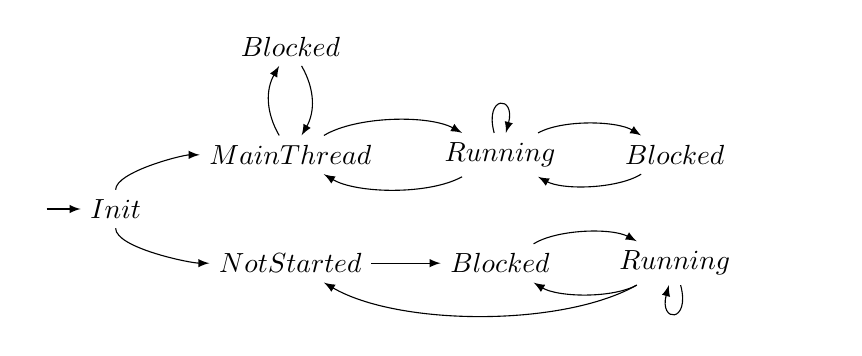
\begin{tikzpicture}
    \node at (9cm,0) (width) {};
    \node at (0,1.5cm) (height) {};

    \path (0,0) --
    node[pos=0.00] (Initxpos) {}
    node[pos=0.25] (Interpreterxpos) {}
    node[pos=0.55] (Executexpos) {}
    node[pos=0.8] (ExecuteAndPollxpos) {}
    (width);

    \path (0,0) --
    node[pos=0] (threadypos) {}
    node[pos=0.5] (Initypos) {}
    node[pos=1] (mainypos) {}
    node[pos=2] (mainBlockedypos) {}
    (height);

    \path (Initxpos |- Initypos) node (Init) {$Init$} ++(-1cm,0cm) node (start) {};
    \node at (Interpreterxpos |- mainypos) (IMn) {$MainThread$};
    \node at (Executexpos |- mainypos) (MRn) {$Running$};
    \node at (Interpreterxpos |- mainBlockedypos) (MBl) {$Blocked$};
    \node at (ExecuteAndPollxpos |- mainypos) (MB2) {$Blocked$};
    \node at (Interpreterxpos |- threadypos) (NSt) {$NotStarted$};
    \node at (Executexpos |- threadypos) (TBl) {$Blocked$};
    \node at (ExecuteAndPollxpos |- threadypos) (TRn) {$Running$};

    \draw[-latex] (start) to (Init);
    \draw[-latex] (Init) to[out=90,in=180,looseness=0.5] (IMn);
    \draw[-latex] (Init) to[out=270,in=180,looseness=0.5] (NSt);
    \draw[-latex] (IMn) to[bend left,looseness=0.7] (MRn);
    \draw[-latex] (MRn) to[bend left,looseness=0.7] (IMn);
    \draw[-latex] (MRn) to[bend left,looseness=0.7] (MB2);
    \draw[-latex] (MB2) to[bend left,looseness=0.7] (MRn);
    \draw[-latex] (IMn) to[bend left,looseness=1.0] (MBl);
    \draw[-latex] (MBl) to[bend left,looseness=1.0] (IMn);
    \draw[-latex] (NSt) to (TBl);
    \draw[-latex] (TBl) to[bend left,looseness=0.7] (TRn);
    \draw[-latex] (TRn) to[bend left,looseness=0.7] (TBl);
    \draw[-latex] (TRn) to[bend left,looseness=0.7] (NSt);
    \draw[-latex] (TRn) to[loop below] (TRn);
    \draw[-latex] (MRn) to[loop above] (MRn);
  \end{tikzpicture}
  \caption{The overall control flow of $Thr$}
  \label{interpreter-flow-figure}
\end{figure}


The $MainThread$ action is shown below.
It begins by accepting a $StackID$ from the $Launcher$ on the
$initMainThread$ channel, which is used to initialise the
$frameStackID$ state component.
It then offers a choice of executing a method on the $main$ thread in
response to a request from the $Launcher$, or switching to another
thread.
A request to start execution of a method is handled in the
$StartIntepreter$ action, which creates the $StackFrame$ for the
method.
The process then behaves as the $Running$ action, executing bytecode
instructions until the method has finished, after which the
$MainThread$ action recurses to offer the choice of method execution
and thread switch again.
If an instruction to switch to another thread from the scheduler is
received on the $CEEswitchThread$ channel, then it is only accepted if
the thread switched from is the $thread$ represented by the process.
If it is accepted, then the process behaves as $Blocked$, waiting for
a request to switch back to the thread, after which it recurses back
to offer the choice of behaviours again.
\begin{circusaction}
  MainThread \circdef initMainThread?stack \then frameStackID := Initialised~stack \circseq \circmu X \circspot \\
  \t1 \circblockbegin
  StartInterpreter \circseq Running \circseq X \\
  {} \extchoice {} \\
  CEEswitchThread?from?to \prefixcolon (from = thread) \then Blocked \circseq X
  \circblockend
\end{circusaction}

The $StartIntepreter$ action, used by $MainThread$ also handles
special methods that execute nested methods.
Its definition is shown below.
It accepts communication on the $executeMethod$ channel, requiring the
$ThreadID$ communicated to be the same as that of the current thread,
$thread$, and storing the other values communicated as $classID$,
$methodID$ and $methodArgs$.
A data operation $ResolveMethod$ is then used to determine the
appropriate class information for the method, since the method may
actually be defined in a superclass of the provided $classID$.
$ResolveMethod$ follows the method resolution rules of the JVM
specification, first checking if the class corresponding to $classID$
defines the method, then checking if one of its superclasses defines
the method, and finally looking for the method definition among its
superinterfaces.
The $Class$ information resulting from this is stored in $class$ and
used to create a new $StackFrame$ on the $frameStack$ in
$InterpreterNewStackFrame$.
The $baseFrame$ value for this stack frame is set to $\true$, since it
is being created in reponse to an external request.
\begin{circusaction}
  StartInterpreter \circdef \\
  \t1  \circvar classID : ClassID; methodID : MethodID; methodArgs : \seq Word; class : Class \circspot \\
  \t1 executeMethod?t \prefixcolon (t = thread) ?c?m?a \then classID, methodID, methodArgs := c, m, a \circseq \\
  \t1 \lschexpract ResolveMethod[cs/cs?] \rschexpract \circseq \lschexpract \exists baseFrame? == \true @ InterpreterNewStackFrame \rschexpract
\end{circusaction}

For threads other than $main$, the behaviour is described by the
$NotStarted$ action below.
It accepts a request to start the $thread$ represented by the process
from the scheduler on the $CEEstartThread$ channel.
The identifier, $bsid$, of the thread's backing store is then passed
to $ObjMan$ via the $addThreadMemory$ channel and the $stack$
identifier is used to initialise $frameStackID$.
The remaining information is stored in $classID$, $methodID$ and
$methodArgs$, and the $Class$ information is determined and a new
$StackFrame$ is created, similarly to what happends in
$StartInterpreter$. 
The process then behaves as the $Blocked$ action, waiting for an
instruction to switch to that thread, after which it behaves as the
$Running$ action, executing bytecode instructions.
When the execution of the thread's method has finished, the scheduler
is signalled on the $CEEremoveThread$ channel.
This causes the scheduler to switch to a different thread, so a thread
switch is accepted on the $CEEswitchThread$ channel.
After that, the action recurses to allow the thread to be restarted.
\begin{circusaction}
  NotStarted \circdef \\
  \t1 \circvar classID : ClassID; methodID : MethodID; methodArgs : \seq Word; class : Class \circspot \\
  \t1 CEEstartThread?toStart?bsid?stack?cid?mid?args \prefixcolon (toStart = thread) \then {} \\
  \t1 addThreadMemory!thread!bsid \then {} \\
  \t1 frameStackID, classID, methodID, methodArgs := Initialised~stack, cid, mid, args \circseq \\
  \t1 \lschexpract ResolveMethod[cs/cs?] \rschexpract \circseq \lschexpract \exists baseFrame? == \true @ InterpreterNewStackFrame \rschexpract \circseq \\
  \t1 Blocked \circseq Running \circseq CEEremoveThread!thread \then {} \\
  \t1 CEEswitchThread?from?to \prefixcolon (from = thread) \then NotStarted
\end{circusaction}

The $Blocked$ and $Running$ actions define the behaviour of threads
after they have been started.
The $Blocked$ action simply waits for a signal on the
$CEEswitchThread$ channel to switch to $thread$, after which it
terminates to allow execution in a different action to continue.
\begin{circusaction}
  Blocked \circdef CEEswitchThread?from?to \prefixcolon (to = thread) \then \Skip
\end{circusaction}

The $Running$ action, shown below, executes the bytecode instructions
of a program. 
It has the form of a loop that repeatedly executes until $frameStack$
is empty.
Within the loop, it handles the bytecode instruction at the current
$pc$ value in $HandleInstruction$ and then it polls for thread
switches in $Poll$.
\begin{circusaction}
  Running \circdef \\
  \t1 \circif frameStack = \emptyset \circthen \Skip \\
  \t1 {} \circelse frameStack \neq \emptyset \circthen HandleInstruction \circseq Poll \circseq Running \\
  \t1 \circfi
\end{circusaction}
The behaviour of polling for thread switches in $Poll$ permits thread
switches inbetween bytecode instructions.
Implementations that allow thread switches at other points are valid
if they retain the same sequence of externally visible events, meaning
only instructions involving communication with other parts of the
model need be atomic.
$Poll$ simply offers communication from the scheduler on the
$CEEswitchThread$ and $CEEproceed$ channels, switching to $Blocked$
upon receiving a signal on $CEEswitchThread$, and terminating on
receiving a signal on $CEEproceed$.

The $HandleInstruction$ action, shown in part below, offers a choice
of actions for handling the bytecode instructions.
There is one action for each of the instructions, with the action's
name formed from the bytecode mnemonic prefixed with $Handle$ (e.g.\
$HandleAload$ for the \texttt{aload} instruction).
\begin{circusaction}
	HandleInstruction \circdef \\
	\t1 HandleAconst\_null \extchoice HandleDup \extchoice HandleAload \extchoice HandleAstore \extchoice HandleIadd \extchoice {} \cdots
\end{circusaction}

The $Handle$ actions define the semantics for the instructions and, as
such are involved in the compilation strategy.
Many of these actions for handling bytecode instructions have a
similar form.

\subsubsection*{Bytecode Semantics}

The simplest $Handle$ actions consist of a guard requiring the $bc$
value at the current $pc$ to be a particular bytecode instruction,
followed by a data operation specified by a Z schema updating
$InterpreterState$.
This is illustrated in the definition of $HandleAconst\_null$ below,
which uses the $InterpreterAconst\_null$ schema.
\begin{circusaction}
  HandleAconst\_null \circdef \lcircguard bc~pc = aconst\_null \rcircguard \circguard \lschexpract InterpreterAconst\_null \rschexpract
\end{circusaction}
The \Circus{} actions and Z schemas for each bytecode instruction are
listed in Table~\ref{bytecode-model-table}.
We omit the definitions of the Z schemas in our description here.
Their contents are in line with the state updates for the bytecode
instructions presented in Table~\ref{bytecode-subset-table}.

\begin{table}[ht]
  \centering
  \begin{tabular}{llp{5cm}}
    \hline
    Bytecode instruction & \Circus{} action & Z schema \\
    \hline
    \texttt{aconst\_null} & $HandleAconst\_null$ & $InterpreterAconst\_null$ \\
    \texttt{aload} & $HandleAload$ & $InterpreterAload$ \\
    \texttt{areturn} & $HandleAreturn$ & $InterpreterAreturn$ \\
    \texttt{astore} & $HandleAstore$ & $InterpreterAstore$ \\
    \texttt{dup} & $HandleDup$ & $InterpreterDup$ \\
    \texttt{getfield} & $HandleGetfield$  & $InterpreterPush$ \\
    \texttt{getstatic} & $HandleGetstatic$ & $InterpreterPush$ \\
    \texttt{goto} & $HandleGoto$ & $InterpreterGoto$ \\
    \texttt{iadd} & $HandleIadd$ & $InterpreterIadd$ \\
    \texttt{iconst} & $HandleIconst$ & $InterpreterPush$ \\
    \texttt{if\_icmple} & $HandleIf\_icmple$ & $InterpreterIf\_icmple$ \\
    \texttt{ineg} & $HandleIneg$ & $InterpreterIneg$ \\
    \texttt{invokespecial} & $HandleInvokespecial$ & $InterpreterStackFrameInvoke$, $InterpreterNewStackFrame$ \\
    \texttt{invokestatic} & $HandleInvokestatic$ & $InterpreterStackFrameInvoke$, $InterpreterNewStackFrame$ \\
    \texttt{invokevirtual} & $HandleInvokevirtual$ & $InterpreterStackFrameInvoke$, $InterpreterNewStackFrame$ \\
    \texttt{new} & $HandleNew$ & $InterpreterPush$ \\
    \texttt{putfield} & $HandlePutfield$ & $InterpreterPop2$ \\
    \texttt{putstatic} & $HandlePutstatic$ & $InterpreterPop$ \\
    \texttt{return} & $HandleReturn$ & $InterpreterReturn$ \\
    \hline
  \end{tabular}
  \caption{The relationship between the bytecode instructions in our
    subset and the \Circus{} actions and Z schemas defining them}
  \label{bytecode-model-table}
\end{table}

The $HandleDup$, $HandleIadd$ and $HandleIneg$ actions follow the
simple form exemplified above.
Some instructions have parameters that must be extracted so that they
can be passed to the data operation for the instruction.
This can be seen in the definition of the $HandleAload$ action, shown
below, in which the inverse of the $aload$ constructor is used to
extract its parameter into a $variableIndex$ variable that is used by
the $IntepreterAload$ schema.
\begin{circusaction}
  HandleAload \circdef  \lcircguard bc~pc \in \ran aload \rcircguard \circguard \\
  \t1 \circvar variableIndex : \nat \circspot variableIndex := (aload\inv)~(bc~pc) \circseq \lschexpract InterpreterAload \rschexpract
\end{circusaction}
The $HandleAstore$, $HandleGoto$, $HandleIconst$ and
$HandleIf\_icmple$ actions all follow a similar form, extracting the
parameter of the bytecode instruction into a separate variable.

The actions to handle the return instructions (\texttt{areturn} and
\texttt{return}) require additional communication to pass the return
value to the $Launcher$ when returning from a method that has been
started by the $Launcher$.
This is performed by an additional action, $CheckLauncherReturn$, that
is called after return from the schema action.
This can be seen in the definition of $HandleAreturn$ below, where
$CheckLauncherReturn$ is passed the two output values from the
$InterpreterAreturn$ function.
The first output, $returnValue$, holds the return value for the
returning method, while the second, $fromBaseFrame$, is a boolean
value indicating if the $StackFrame$ for the method had its
$baseFrame$ value set to $\true$.
\begin{circusaction}
  HandleAreturn \circdef \circvar returnValue : Word; fromBaseFrame : \boolean \circspot \\
  \t1 \lcircguard bc~pc = areturn \rcircguard \circguard \lschexpract InterpreterAreturn \rschexpract \circseq \\
  \t1 CheckLauncherReturn(returnValue, fromBaseFrame)
\end{circusaction}
The form of the $HandleReturn$ action is similar, but since
$InterpreterReturn$ does not output a return value, $returnValue$
takes an arbitrary value.

Within the $CheckLauncherReturn$ action, the definition of which is
shown below, the boolean value $fromBaseFrame$ is used to determine
whether the return value should be communicated to the $Launcher$.
If $fromBaseFrame$ is set to $\true$, then that normally indicates
that the return value needs to be passed to the launcher.
The exception to this is if the return is from the first frame of a
$thread$ other than $main$, which is created in response to a
$CEEstartThread$ signal from the scheduler and so does not require a
return value to be sent to the launcher.
Thus, the condition checked is that $fromBaseFrame$ is $\true$, and
either $frameStack$ is empty or the current $thread$ is $main$.
If that is true, then $returnValue$ is sent to the $Launcher$ on the
$executeMethodRet$ channel and a signal is awaited on the
$continueExecution$ channel before continuing.
If the condition is not true then the action terminates.
\begin{circusaction}
  CheckLauncherReturn \circdef \circval returnValue : Word; \circval fromBaseFrame : \boolean \circspot \\
  \t1 \circif fromBaseFrame = \true \land (frameStack \neq \emptyset \lor thread = main) \circthen \\
  \t2 executeMethodRet!thread!returnValue \then continueExecution?t \prefixcolon (t = thread) \then \Skip \\
  \t1 {} \circelse fromBaseFrame = \false \lor (frameStack = \emptyset \land thread \neq main) \circthen \Skip \\
  \t1 \circfi
\end{circusaction}

For the instructions that create objects and access their fields
(\texttt{new}, \texttt{getfield}, \texttt{putfield},
\texttt{getstatic} and \texttt{putstatic}), communication with
$ObjMan$ is needed.
This can be seen in the definition of $HandleGetfield$, shown below,
where the object identifier, $oid$, is popped from the $operandStack$
of the current $StackFrame$ using the data operation $IntepreterPop$,
and the field identifier is extracted from the parameter to the
bytecode instruction.
Note that $pc$ is hidden from the $InterpreterPop$, since this action
uses two data operations promoted from $StackFrame$ operations and
only one of them need update $pc$. 
This information is passed to $ObjMan$ via the $getField$ channel,
which then handles the operation.
The field's value is returned via the $getFieldRet$ channel and pushed
onto the $operandStack$ of the current $StackFrame$ by the data
operation $InterpreterPush$.
\begin{circusaction}
  HandleGetfield \circdef \lcircguard bc~pc \in \ran getfield \land (getfield\inv)~(bc~pc) \in fieldRefIndices~currentClass \rcircguard \circguard \\
  \t1 \circvar oid : ObjectID \circspot \lschexpract InterpreterPop[oid!/value!] \hide (pc, pc') \rschexpract \circseq \\
  \t1 getField!oid!(fieldOf~currentClass~((getfield\inv)~(bc~pc))) \\
  \t1 {} \then getFieldRet?value \then \lschexpract InterpreterPush \rschexpract
\end{circusaction}
The $HandleNew$, $HandlePutfield$, $HandleGetstatic$ and
$HandlePutstatic$ actions are similar, getting information from the
$operandStack$ using $InterpreterPop$, communicating with $ObjMan$ to
handle the instruction, and using $InterpreterPush$ to push returned
information onto the $operandStack$.

Finally, the method invocation instructions (\texttt{invokespecial},
\texttt{invokestatic} and \texttt{invokevirtual}), require special
handling by the virtual machine.
Since the different method invocation instructions differ only in how
the class for the method is determined and whether a \texttt{this}
object identifier is passed among the method's arguments, the
invocation of the method after this has been determined is handled by
a common $Invoke$ action.
This can be seen in the definition of the $HandleInvokespecial$ action
below.
The method identifier $mid$ is extracted from the instruction's
parameter, and the data operation $InterpreterStackFrameInvoke$ is
used to store the return $pc$ address and pop the arguments of the
method in $poppedArgs$.
The number of arguments popped, $argsToPop?$, is the $methodArguments$
value for $mid$, plus one for the \texttt{this} identifier passed to
the method.
The class identifier is then extracted from the instruction's
parameter and passed into $Invoke$ along with $mid$ and $poppedArgs$.
\begin{circusaction}
  HandleInvokespecial \circdef \circvar cid : ClassID; mid : MethodID; poppedArgs : \seq Word \circspot \\
  \t1 \lcircguard bc~pc \in \ran invokespecial \land ((invokespecial\inv)~(bc~pc)) \in methodRefIndices~currentClass \rcircguard \circguard \\
  \t1 mid := methodOf~currentClass~((invokespecial\inv)~(bc~pc)) \circseq \\
  \t1 \lschexpract \exists argsToPop? == methodArguments~mid + 1 @ InterpreterStackFrameInvoke \rschexpract \circseq \\
  \t1 Invoke(classOf~currentClass~((invokespecial\inv)~(bc~pc)), mid, poppedArgs)
\end{circusaction}
The $HandleInvokestatic$ and $HandleInvokevirtual$ actions are
similar, except that $argsToPop?$ does not include the extra
\texttt{this} argument in $HandleInvokeStatic$, and
$HandleInvokevirtual$ obtains the class identifier from the
\texttt{this} identifier via the $getClassIDOf$ channel rather than
from the instruction's parameter.

The $Invoke$ action, shown in part below, has the form of an external
choice over actions for each of the special methods supported by the
SCJVM, plus an $InvokeOther$ action for handling non-special methods
implemented in bytecode.
The name of the action for each special method is formed from the name
of the special method prefixed with $Invoke$ (e.g. 
$InvokeResumeThread$ for the \texttt{resumeThread()} method).
The parameters passed to the $Invoke$ action, which are the class
identifier, $classID$, the method identifier, $method$, and the
method argument list, $args$, are passed on to each of the actions in
the external choice.
\begin{circusaction}
  Invoke \circdef \circval classID : ClassID; \circval method : MethodID; \circval args : \seq Word \circspot \\
  \t1 InvokeResumeThread(classID, method, args) \extchoice InvokeSuspend(classID, method) \extchoice \cdots \\
  \t1 {} \extchoice InvokeOther(classID, method, args)
\end{circusaction}

Within the special method actions, there is a guard ensuring the
action is taken when the class and method identifiers are those for
the method.
The method is then handled by communication on the appropriate
channels.
This is illustrated by the definition of the $InvokeResumeThread$
action, shown below.
The class identifier parameter, $classID$, is required to refer to a
subclass of some class $resumeThreadClass$, while the method
identifier, $method$, must be $resumeThreadID$.
The class and method identifiers used in the special method actions
are a mixture of identifiers from the SCJ API and
implementation-defined identifiers provided to expose SCJVM services
to bytecode programs.
The argument to the method, stored as the first element of the
$methodArgs$ parameter, is converted to a $ThreadID$ and passed to the
$Launcher$ via the $resumeThread$ channel.
A return signal is then awaited on the $resumeThreadRet$ channel
before continuing.
\begin{circusaction}
  InvokeResumeThread \circdef \\
  \t1 \circval classID : ClassID; \circval method : MethodID; \circval methodArgs : \seq Word \circspot \\
  \t1 \lcircguard (classID,resumeThreadClass) \in subclassRel~cs \land method = resumeThreadID \rcircguard \circguard {} \\
  \t1 resumeThread!(WordToThreadID~(methodArgs~1)) \then resumeThreadRet \then \Skip
\end{circusaction}

Some of the special methods start other methods as part of their
execution, which requires additional handling.
An example is \texttt{enterPrivateMemory()} from the SCJ API, which
executes the \texttt{run()} method of a \texttt{Runnable} object after
entering a private memory area.
This is handled in the action $InvokeEnterPrivateMemory$, shown below.
It begins in a similar way to $InvokeResumeThread$, with a guard on
the $classID$ and $method$ passed into the action.
The method is then handled by communicating with the $Launcher$ on the
$enterPrivateMemory$ channel, passing the arguments from $methodArgs$.
The execution of the nested method is then handled as in
$StartInterpreter$, waiting for the request to execute the nested
method on the $executeMethod$ channel and creating a new $StackFrame$
for it.
\begin{circusaction}
  InvokeEnterPrivateMemory \circdef \\
  \t1 \circval classID : ClassID; \circval method : MethodID; \circval methodArgs : \seq Word \circspot \\
  \t1 \lcircguard (classID,managedMemoryClass) \in subclassRel~cs \land method = enterPrivateMemoryID \rcircguard \circguard {} \\
  \t2 enterPrivateMemory!thread!(methodArgs~1)!(methodArgs~2) \then StartInterpreter
\end{circusaction}

In addition to the special methods handled in the $Launcher$, we also
supply \texttt{read()} and \texttt{write()} methods for reading from
and writing to some standard input and output device. 
These methods are handled using the \texttt{input} and \texttt{output}
channels that communicate the values from and to the environment of
the SCJVM.
This is shown in the definition of the $InvokeRead$ action below,
which accepts the input on the $input$ channel and pushes it onto the
stack as the return value for the method.
\begin{circusaction}
  InvokeRead \circdef \\
  \t1 \circval classID : ClassID; \circval method : MethodID; \circval methodArgs : \seq Word \circspot \\
  \t1 \lcircguard (classID,readClass) \in subclassRel~cs \land method = readID \rcircguard \circguard {} \\
  \t2 input?value \then \lschexpract InterpreterPush \hide (pc,pc') \rschexpract
\end{circusaction}
The $InvokeWrite$ action is similar, writing the method argument to
the $output$ channel.

The $InvokeOther$ action, shown in part below, describes the handling
of non-special methods.
It begins with a guard that is the conjunction of the negation of the
guards for the invocation actions for the special methods.
The actions starts execution of the method in the interpreter by
finding its $Class$ information with $ResolveMethod$ and creating a
new $StackFrame$ with $IntepreterNewStackFrame$.
The $baseFrame$ value is set to $\false$ here, since the stack frame
is created due to execution of a bytecode instruction in the
interpreter, rather than in response to an external request.
\begin{circusaction}
  InvokeOther \circdef \circval classID : ClassID; \circval methodID : MethodID; \circval methodArgs : \seq Word \circspot \\
  \t1 \lcircguard ((classID,resumeThreadClass) \notin subclassRel~cs \lor methodID \neq resumeThreadID) \\
  \t2 {} \land \cdots \\
  \t2 {} \land ((classID, writeClass) \notin subclassRel~cs \lor methodID \neq writeID) \rcircguard \circguard {} \\
  \t1 \circvar class : Class \circspot \\
  \t1 \lschexpract ResolveMethod[cs/cs?] \rschexpract \circseq \lschexpract \exists baseFrame? == \false @ InterpreterNewStackFrame \rschexpract
\end{circusaction}

This concludes our description of the handling of bytecode
instructions, and of our description of the CEE before the application
of the compilation strategy.
In the next section we describe the model of the C code that is used
for the output of the compilation strategy.

\section{C Code Model}
\label{cee-c-code-section}

As mentioned previously, the CEE after compilation to C has a similar
structure to the CEE before compilation, but the object manager is
replaced with a struct manager and the intepreter is replaced with the
C program.
The struct manager is represented by a process $StructMan_{cs}$, and
the C program by a process $CProg_{bc,cs}$.
These are place in parallel composition with the $Launcher$ process
described in Section~\ref{cee-launcher-section} to form a $CCEE_{bc,cs}$
process representing the CEE for a C program, as shown below.
\begin{circus}
  CEE_{bc,cs}(sid, initOrder) \circdef StructMan_{cs} \parallel CProg_{bc,cs} \parallel Launcher(sid, initOrder)
\end{circus}
The subscripts here indicate that the processes depend on the $bc$ and
$cs$ constants used as inputs to the compilation strategy. 
However, $bc$ and $cs$ are not true parameters of the processes and so
are not referenced within the processes.
Note that the $sid$ and $initOrder$ parameters to $Launcher$ remain as
parameters here since $Launcher$ is not transformed during the
compilation strategy.

The channels used for communication between these processes are the
same as those in Table~\ref{cee-channel-table}, except that the
$getField$, $getFieldRet$ and $putField$ channels are replaced with
$getObject$, $getObjectRet$ and $putObject$ channels.
The new channels are discussed in more detail in the
Section~\ref{cee-struct-manager-subsection}, which describes the
struct manager.
After that, in Section~\ref{cee-c-program-subsection}, the
$CProg_{bc,cs}$ process is described and the shallow embedding of C it
uses is discussed.

\subsection{Struct Manager}
\label{cee-struct-manager-subsection}

$StructMan_{cs}$ manages objects represented by C structs that
incorporate the class information from $cs$, refining the process
$ObjMan$, which handles abstract objects.
$StructMan_{cs}$ has Z schemas representing struct types for objects
of each class.
For each class identifier ${<}classID_1{>}, \dots, {<}classID_n{>}$,
we define a schema ${<}classID_k{>}Obj$ for $k \in \{1,\dots,n\}$,
representing the objects of that class. 
They begin with a $classID$ component containing the class identifier
of the object, so that polymorphic method calls can be made by choice
over the object's class.
There is then a component for each of the fields
${<}fieldID_1{>}, \dots, {<}fieldID_{m_k}{>}$ of the class, with each
component having the type $Word$.
\begin{schema}{{<}classID_k{>}Obj}
  classID : ClassID \\
  {{<}fieldID_{k,1}{>}} : Word \\
  \t1 \vdots \\
  {{<}fieldID_{k,m_k}{>}} : Word
\end{schema}

The schema types for each type of object are combined into a single
free type $ObjectStruct$.
The constructor for each ${<}classID_k{>}$ is called
${<}classID_k{>}Con$, with a single parameter of type
${<}classID_k{>}Obj$.
\begin{zed}
  ObjectStruct ::= {<}classID_1{>}Con \ldata {<}classID_1{>}Obj \rdata | \dots | {<}classID_n{>}Con \ldata {<}classID_n{>}Obj \rdata
\end{zed}

For each object type, we define a natural number constant
$sizeof{<}classID_k{>}Obj$ that represents the result of applying C's
\texttt{sizeof} operator to the struct represented by the
corresponding ${<}classID_k{>}Obj$ type.
We also define a function $classIDOf$ for obtaining the value of the
common $classID$ field from an $ObjectStruct$ value.
Additionally, we define a $cast{<}classID_k{>}$ function for each
${<}classID_k{>}$, which maps an $ObjectStruct$ value to a
${<}classID_k{>}Obj$ value.
This works not only for values in the range of the
${<}classID_k{>}Con$ constructor, but also for any class that is a
subclass of ${<}classID_k{>}$, with the common fields copied across.
Thus, $cast{<}classID_k{>}$ represents casting of C structs, where a
struct can be truncated by casting to a struct whose fields are a
prefix of it.
Finally, we also define a function
$update{<}classID_k{>}\_{<}fieldID{>}_i$ for each class identifier
${<}classID_k{>}$ and field identifier ${<}fieldID_i{>}$, which takes
an $ObjectStruct$ and updates the specified field with a given value.
This represents a combined cast and update.

Channels $getObject$, $getObjectRet$, and $putObject$, the definitions
of which are shown below, are used to pass $ObjectStruct$ values to
and from $StructMan_{cs}$.
\begin{circus}
  \circchannel getObject : ObjectID \\
  \circchannel getObjectRet : ObjectStruct \\
  \circchannel putObject : ObjectID \cross  ObjectStruct
\end{circus}

For the static class fields, the static fields from each class
${<}classID_1{>}, \dots, {<}classID_n{>}$ are collected together in a
schema $StaticFields$, as shown below.
\begin{schema}{StaticFields}
  {<}classID_1{>}\_{<}staticfieldID_{1,1}{>} : Word \\
  \t1 \vdots \\
  {<}classID_1{>}\_{<}staticfieldID_{1,\ell_1}{>} : Word \\
  \t1 \vdots \\
  {<}classID_n{>}\_{<}staticfieldID_{n,1}{>} : Word \\
  \t1 \vdots \\
  {<}classID_n{>}\_{<}staticfieldID_{n,\ell_n}{>} : Word
\end{schema}
We define a natural number constant $sizeofStaticFields$ giving the
amount of space required for the struct represented by $StaticFields$.

The $StaticFields$ type is communicated using the $getStaticFields$
and $putStaticFields$ channels, the definitions of which are shown
below.
\begin{circus}
  \circchannel getStaticFields : StaticFields \\
  \circchannel putStaticFields : StaticFields
\end{circus}

The state of $StructMan_{cs}$ is given by the schema $StructManState$,
shown below.
This is similar to $ObjManState$, but the $objects$ map relates object
identifiers to $ObjectStruct$ values, and $staticClassFields$ is a map
from $ObjectID$ to the $StaticFields$ type.
We omit the invariant as it is similar to the invariant of
$ObjManState$.
\begin{schema}{StructManState}
  objects : ObjectID \pfun ObjectStruct \\
  backingStoreMap : BackingStoreID \pfun \finset ObjectID \\
  backingStoreStacks : ThreadID \pfun \seq_1 BackingStoreID \\
  rootBS : BackingStoreID \\
  staticClassFieldsID : StaticFieldsStructID \\
  staticClassFields : ObjectID \pfun StaticFields
\where
  \dots
\end{schema}

Within the $StructMan_{cs}$ process, the structure is much the same as
for the $ObjMan$ process, with the state initialised in the same way.
However, $AllocateStaticFields$ is changed to handle the
$StaticFields$ type.
The definition of $AllocateStaticFields$ in $StructMan_{cs}$ is as
shown below.
It is similar to the $ObjMan$ definition of $AllocateStaticFields$,
but it does not collect the required field identifiers since that is
already implicitly done in the definition of $StaticFields$.
The required size for the allocated space is now $sizeofStaticFields$.
The initialisation of the static fields, in $InitStaticFields$ is much
the same, but now specialised to refer to $StaticFields$, setting all
its components to $null$.
\begin{circusaction}
  AllocateStaticFields \circdef \\
  \t1 MMallocateMemory!(last~(backingStoreStacks~main))!(sizeofStaticFields) \then {} \\
  \t1 MMallocateMemoryRet?objectID \then {} \\
  \t2 (MMreport?r \prefixcolon (r = MMokay) \then \lschexpract InitStaticFields \rschexpract \\
  \t2 {} \extchoice MMreport?r \prefixcolon (r = MMokay) \then \Chaos)
\end{circusaction}

Also, the actions $GetField$, $PutField$, $GetStatic$ and $PutStatic$
are replaced with new actions $GetObject$, $PutObject$, $GetStaticFields$ and
$PutStaticFields$.
These are fairly simple, with $GetObject$ and $PutObject$ retrieving
and storing $ObjectStruct$ values in the $objects$ map.
These are presented exposed on the $getObject$ and $getObjectRet$
channels for $GetObject$, and the $putObject$ channel for $PutObject$. 
Similarly, $GetStaticFields$ and $PutStaticFields$ retrieve and store
the $StaticFields$ value associated with $staticClassFieldsID$ from
the $staticClassFields$ map.
These are performed on the $getStaticFields$ and $putStaticFields$
channels respectively.
We omit the definitions of these actions here; their definitions are
given in Appendix~\ref{struct-manager-appendix}, which shows the
general form of the $StructMan_{cs}$ process.

The $NewObject$ action is different in $StructMan_{cs}$ to that in
$ObjMan$. 
It uses the same channels ($newObject$ and $newObjectRet$), but must
create the correct $ObjectStruct$ value for the provided class.
It has the form shown below.
The $thread$ and $classID$ identifiers are received from the
$newObject$ channel, and a choice is then made over the $classID$,
matching it against each class identifier supported by
$StructMan_{cs}$.
If $classID$ matches a class identifier ${<}classID_k{>}$, then space
for the object is allocated via communication with the memory manager,
as in $AllocateStaticFields$, then the object is stored in $objects$
and initialised.
The allocation is performed in a separate action, $AllocateObject$, as
it is similar for each class.
The size of the object is given by the $sizeof{<}classID_k{>}$
identifier for ${<}classID_k{>}$, and the returned object identifier
is stored in $objectID$.
The storing and initialisation of the object is then done in a schema
action $StructMan{<}classID_k{>}ObjInit$, which sets all the object's
fields to $null$ and puts it in $objects$, stored within
${<}classID_k{>}Con$. 
Finally, $objectID$ is returned via the $newObjectRet$ channel.
\begin{circusaction}
  NewObject \circdef \circvar objectID : ObjectID \circspot \\
  \t1 newObject?thread?classID \then \\
  \t1 \circif classID = {{<}classID_1{>}} \circthen {} \\
  \t2 AllocateObject(thread, sizeof{<}classID_1{>}, objectID) \circseq \lschexpract StructMan{<}classID_1{>}ObjInit \rschexpract \\
  \t1 {} \circelse classID = {{<}classID_2{>}} \circthen {} \\
  \t2 AllocateObject(thread, sizeof{<}classID_2{>}, objectID) \circseq \lschexpract StructMan{<}classID_2{>}ObjInit \rschexpract \\
  \t2 \vdots \\
  \t1 {} \circelse classID = {{<}classID_n{>}} \circthen {} \\
  \t2 AllocateObject(thread, sizeof{<}classID_n{>}, objectID) \circseq \lschexpract StructMan{<}classID_n{>}ObjInit \rschexpract \\
  \t1 \circfi \circseq newObjectRet!objectID \then \Skip \\
\end{circusaction}

Finally, $GetClassIDOf$ is changed to extract the class identifier
from an $ObjectStruct$ value using the $classIDOf$ function.
This is not used in the C code, which, as we will see in the next
section, uses $classIDOf$ directly, but is supplied for use by the
$Launcher$, which is unchanged by the strategy.
We omit the definition of $GetClassIDOf$ here.

In the next section we describe the structure of the C code of the
program and our shallow embedding of C in \Circus{}, which makes use
of some of the types and channels discussed in this section.

\subsection{Shallow Embedding of C in \Circus{}}
\label{cee-c-program-subsection}

The C code output by our compilation strategy is represented by a
\Circus{} process $CProg_{bc,cs}$, which is determined by the bytecode
instructions, $bc$, and the class information, $cs$.
This process has a similar structure to that of $Interpreter$:~a
parallel composition of $CThr_{bc,cs}(t)$ processes representing C
threads, one for each thread identifier $t$ except the $idle$ thread,
as shown in the definiton of $CProg_{bc,cs}$ below.
\begin{circus}
  \circprocess CProg_{bc,cs} \circdef \Parallel t : ThreadID \setminus \{ idle \} \lpar ThrChans(t) \rpar \circspot CThr_{bc,cs}(t)
\end{circus}

The $CThr_{bc,cs}$ process has a similar structure to the $Thr$
process presented in Section~\ref{cee-interpreter-subsection}.
However, the $pc$ and $frameStack$ components are eliminated from the
state during compilation.
Thus, the state of $CThr_{bc,cs}$, shown in $CThrState$ below, just
contains $stackID$, which has the same type as $frameStackID$ in
$InterpreterState$ and so may be $Uninitialised$ or $Initialised$ with
a $StackID$ for the C thread's stack.
Since there is no explicit stack in C, we only need to ensure there is
a stack identifier in $stackID$ so space for the thread's stack has
been allocated and the $stackID$ is not manipulated beyond that.
\begin{schema}{CThrState}
  stackID : Stack
\end{schema}
The $stackID$ is initially set to $Uninitialised$.

The $Running$ action and creation of stack frames are also replaced
with an $ExecuteMethod$ action that executes the C function
corresponding to a given method identifier.
The main action of $CThr_{bc,cs}$ thus has the same structure as that
of $Interpreter$, with a choice of $MainThread$ for the $main$ thread
and $NotStarted$ for non-$main$ threads.
However, $MainThread$ now has the structure shown below.
This is similar to the definition of $MainThread$ in $Thr$, but the
information received from the $executeMethod$ channel is passed into
the $ExecuteMethod$ action to select the correct C function to
execute.
After method execution has finished, the return value, $retVal$, is
obtained from $ExecuteMethod$ and communicated on the
$executeMethodRet$ channel.
\begin{circusaction}
  MainThread \circdef initMainThread?stack \then stackID := Initialised~stack \circseq \circmu X \circspot \\
  \t1 \circblockbegin
  \circvar retVal : Word \circspot executeMethod?t \prefixcolon (t = thread) ?cid?mid?args \then {} \\
  \t1 ExecuteMethod(cid,mid,args,retVal) \circseq \\
  \t1 executeMethodRet!retVal \then continueExecution \then X \\
  {} \extchoice {} \\
  CEEswitchThread?from?to \prefixcolon (from = thread) \then Blocked
  \circseq X \circblockend
\end{circusaction}

Similarly, the $NotStarted$ action in $CThr_{bc,cs}$ has the form
shown below, with $ExecuteMethod$ after $Blocked$, replacing
$Running$.
The return value, $retVal$, is discarded here since the methods that
are executed a the top level on the non-$main$ threads should not
return a value so $retVal$ will be arbitrary.
The thread's removal is also handled by $CEEremoveThread$ so no
communication on $executeMethodRet$ follows the end of the method's
execution.
\begin{circusaction}
  NotStarted \circdef \\
  \t1 \circvar classID : ClassID; methodID : MethodID; methodArgs : \seq Word; class : Class \circspot \\
  \t1 CEEstartThread?toStart?bsid?stack?cid?mid?args \prefixcolon (toStart = thread) \then {} \\
  \t1 addThreadMemory!thread!bsid \then {} \\
  \t1 frameStackID, classID, methodID, methodArgs := Initialised~stack, cid, mid, args \circseq \\
  \t1 Blocked \circseq \circvar retVal : Word \circspot ExecuteMethod(classID, methodID, methodArgs, retVal) \circseq \\
  \t1 CEEremoveThread!thread \then CEEswitchThread?from?to \prefixcolon (from = thread) \then NotStarted
\end{circusaction}

The $ExecuteMethod$ action has the form shown below.
It takes as parameters the class identifier, $cid$, method identifier,
$mid$, and arguments list, $args$, for the method to be executed.
It then chooses the appropriate action corresponding to the supplied
$cid$ and $mid$, and passes the appropriate number of arguments from
$args$ to the action.
The return value of each of the actions, if they return one, is
captured in $retVal$ to be returned to $MainThread$ or $NotStarted$.
\begin{circusaction}
  ExecuteMethod \circdef \\
  \t1 \circval cid : ClassID; \circval mid : MethodID; \circval args : \seq Word; \circres retVal : Word \circspot \\
  \t1 \circif (cid,mid) = ({<}classID_1{>}, {<}methodID_1{>}) \circthen {} \\
  \t2 {<}classID_1{>}\_{<}methodID_1{>}(args~1,\dots,args~(methodArgs~{<}methodID_1{>}), retVal) \\
  \t2 \vdots \\
  \t1 {} \circelse (cid,mid) = ({<}classID_n{>}, {<}methodID_{m_n}{>}) \circthen {} \\
  \t2 {<}classID_n{>}\_{<}methodID_{m_n}{>}(args~1,\dots,args~(methodArgs~{<}methodID_{m_n}{>}), retVal) \\
  \t1 \circif
\end{circusaction}

The actions used by $ExecuteMethod$ represent C functions containing
the behaviour of the compiled methods.
The name of each action is made up of the class and method identifier
for the method, separated by an underscore.
Within the action, the constructs of C are represented by constructs
of \Circus{}. 
The representation of these constructs is summarised in
Table~\ref{embedding-table}.

\begin{table}[t]
\centering
{\scriptsize
\setlength{\zedindent}{0pt}
\setlength{\zedleftsep}{2mm}
\setlength{\zedtab}{1em}
\setlength{\abovedisplayskip}{0mm}
\setlength{\belowdisplayskip}{0mm}
\setlength{\abovedisplayshortskip}{0mm}
\setlength{\belowdisplayshortskip}{0mm}
\renewcommand{\arraystretch}{0.5}
\rowcolors{2}{white}{lightgray}
\begin{tabular}{p{3cm}p{5cm}p{4cm}}
\hline
Construct & C code & \Circus{} equivalent \\
\hline %%%%%%%%%%%%%%%%%%%%%%%%%%%%%%%%%%%%%%%%%%%%%%%%%%%%%%%%%%%%%%%%
\raggedright \hfill \newline Function definition &
\begin{lstlisting}
void foo() {...}
\end{lstlisting}
&
\[
Foo \circdef \cdots
\] \\
%\hline %%%%%%%%%%%%%%%%%%%%%%%%%%%%%%%%%%%%%%%%%%%%%%%%%%%%%%%%%%%%%%%%
\raggedright \hfill \newline Function definition with argument &
\begin{lstlisting}
void bar(int32_t x) {...}
\end{lstlisting}
&
\[
  Bar \circdef \circval x : Word \circspot \cdots
\] \\
%\hline %%%%%%%%%%%%%%%%%%%%%%%%%%%%%%%%%%%%%%%%%%%%%%%%%%%%%%%%%%%%%%%%
\raggedright \hfill \newline Function definition with return value &
\begin{lstlisting}
int32_t baz() {...}
\end{lstlisting}
&
\[
  Baz \circdef \circres retVal : Word \circspot \cdots
\] \\
% \hline %%%%%%%%%%%%%%%%%%%%%%%%%%%%%%%%%%%%%%%%%%%%%%%%%%%%%%%%%%%%%%%
\raggedright \hfill \newline Function definition with parameter and return value &
\begin{lstlisting}
int32_t quux(int32_t x) {...}
\end{lstlisting}
&
\[
  Quux \circdef \circval x : Word; \\
  \t1 \circres retVal : Word \circspot \cdots
\] \\
% \hline %%%%%%%%%%%%%%%%%%%%%%%%%%%%%%%%%%%%%%%%%%%%%%%%%%%%%%%%%%%%%%%
\raggedright \hfill \newline Function call &
\begin{lstlisting}
foo();
\end{lstlisting}
&
\[
Foo
\] \\
%\hline %%%%%%%%%%%%%%%%%%%%%%%%%%%%%%%%%%%%%%%%%%%%%%%%%%%%%%%%%%%%%%%%
\raggedright \hfill \newline Function call with argument &
\begin{lstlisting}
bar(x);
\end{lstlisting}
&
\[
Bar(x)
\] \\
%\hline %%%%%%%%%%%%%%%%%%%%%%%%%%%%%%%%%%%%%%%%%%%%%%%%%%%%%%%%%%%%%%%%
\raggedright \hfill \newline Function call with return value &
\begin{lstlisting}
x = baz();
\end{lstlisting}
&
\[
Baz(x)
\] \\
%\hline %%%%%%%%%%%%%%%%%%%%%%%%%%%%%%%%%%%%%%%%%%%%%%%%%%%%%%%%%%%%%%%%
\raggedright \hfill \newline Function call with argument and return value &
\begin{lstlisting}
y = quux(x);
\end{lstlisting}
&
\[
Quux(x,y)
\] \\
%\hline %%%%%%%%%%%%%%%%%%%%%%%%%%%%%%%%%%%%%%%%%%%%%%%%%%%%%%%%%%%%%%%%
\raggedright \hfill \newline Return statement &
\begin{lstlisting}
return;
\end{lstlisting}
&
\begin{circus}
\Skip
\end{circus} \\
%\hline %%%%%%%%%%%%%%%%%%%%%%%%%%%%%%%%%%%%%%%%%%%%%%%%%%%%%%%%%%%%%%%%
\raggedright \hfill \newline Return statement with value &
\begin{lstlisting}
return x;
\end{lstlisting}
&
\begin{circus}
  retVal := x
\end{circus} \\
%\hline %%%%%%%%%%%%%%%%%%%%%%%%%%%%%%%%%%%%%%%%%%%%%%%%%%%%%%%%%%%%%%%%
\raggedright \hfill \newline Assignment &
\begin{lstlisting}
x = e;
\end{lstlisting}
&
\begin{circus}
x := e
\end{circus} \\
%\hline %%%%%%%%%%%%%%%%%%%%%%%%%%%%%%%%%%%%%%%%%%%%%%%%%%%%%%%%%%%%%%%%
\raggedright \hfill \newline Variable declaration &
\begin{lstlisting}
int32_t x;
\end{lstlisting}
& \[\circvar x : Word \circspot \] \\
%\hline %%%%%%%%%%%%%%%%%%%%%%%%%%%%%%%%%%%%%%%%%%%%%%%%%%%%%%%%%%%%%%%%
\raggedright \hfill \newline Variable declaration and initialisation &
\begin{lstlisting}
int32_t x = e;
\end{lstlisting}
& \[\circvar x : Word \circspot x := e\] \\
%\hline %%%%%%%%%%%%%%%%%%%%%%%%%%%%%%%%%%%%%%%%%%%%%%%%%%%%%%%%%%%%%%%%
\raggedright \hfill \newline If statement &
\begin{lstlisting}
if (b) {...}
\end{lstlisting}
&
\[
\circif b \circthen \cdots \\
{} \circelse \lnot b \circthen \Skip \\
\circfi
\] \\
%\hline %%%%%%%%%%%%%%%%%%%%%%%%%%%%%%%%%%%%%%%%%%%%%%%%%%%%%%%%%%%%%%%%
\raggedright \hfill \newline If-else statement &
\begin{lstlisting}
if (b) {...} else {...}
\end{lstlisting}
&
\[
\circif b \circthen \cdots \\
{} \circelse \lnot b \circthen \cdots \\
\circfi
\] \\  
%\hline %%%%%%%%%%%%%%%%%%%%%%%%%%%%%%%%%%%%%%%%%%%%%%%%%%%%%%%%%%%%%%%%
\raggedright \hfill \newline Infinite loop &
\begin{lstlisting}
while (1) {...}
\end{lstlisting}
&
{
\[
\circmu X \circspot\cdots \circseq X
\]}\\
%\hline %%%%%%%%%%%%%%%%%%%%%%%%%%%%%%%%%%%%%%%%%%%%%%%%%%%%%%%%%%%%%%%%
\raggedright \hfill \newline While loop &
\begin{lstlisting}
while (b) {...}
\end{lstlisting}
&
{
\def\arraystretch{1.1}
\[
\circmu X \circspot \\
  \t1 \circif b \circthen \cdots \circseq X \\
  \t1 {} \circelse \lnot b \circthen \Skip \\
  \t1 \circfi
\]}\\  
%\hline %%%%%%%%%%%%%%%%%%%%%%%%%%%%%%%%%%%%%%%%%%%%%%%%%%%%%%%%%%%%%%%%
\raggedright \hfill \newline Do-while loop &
\begin{lstlisting}
do {...} while (b);
\end{lstlisting}
&
{
\def\arraystretch{1.1}
\[
  \circmu X \circspot \cdots \circseq \\
  \t1 \circif b \circthen X \\
  \t1 {} \circelse \lnot b \circthen \Skip \\
  \t1 \circfi
\]}\\
\hline %%%%%%%%%%%%%%%%%%%%%%%%%%%%%%%%%%%%%%%%%%%%%%%%%%%%%%%%%%%%%%%%%
\end{tabular}}
\caption{The \Circus{} representations of C constructs in our shallow
  embedding}
\label{embedding-table}
\end{table}

The constructs we allow within a C function are conditionals, while
loops, assignment statements, and function calls.
These are comparable with those allowed in MISRA-C~\cite{MISRA} and
present in the code generated by icecap.
Conditionals in C correspond to \Circus{} alternation blocks, similar
to those in Dikstra's guarded command language~\cite{dijkstra1975}.
We handle loops in C using recursion in \Circus{}, with alternation
used to handle loop conditions.

As each function in the C code is a \Circus{} action, function calls
are represented as references to those actions.
Function arguments in C are passed by value, although those values may
be pointers to other values.
Accordingly, since our SCJVM model represents pointers explicitly (via
the object/struct manager), we represent function arguments using
value parameters of the \Circus{} action.

If a function has a return value, it is represented with a result
parameter of the \Circus{} action, usually named $retVal$, with an
assignment to that parameter at the end of the action representing
return statements.
We assume there is a single return statement at the end of the
function, so the return can simply be represented by the termination
of the action if there is no return value.
It is not necessary to cater for return statements in the middle of a
function as we have control over the structure of the functions.
We follow guidelines for safety-critical uses of C variants, such as
MISRA-C~\cite{MISRA}, and use a single return statement at the end of
a function.
A function with both a return value and arguments has its value
parameters (representing the arguments) followed by the result
parameter (representing the return value).

Local variables of the function are represented using \Circus{}
variable blocks.
These are placed near the start of the action, after the parameter
declarations.
While \Circus{} variable blocks could also be used to represent
variables declared in the middle of functions, that is not necessary
for our work.
Restricting ourselves to variables at the start of functions ensures
the code or strategy generates is compatible with older versions of C.


\section{Final Considerations}
\label{cee-final-considerations-section}

In this chapter we have presented our model of the core execution
environment (CEE) of an SCJVM and specified the subset of Java
bytecode covered in our model.
Our bytecode subset consists of 14 instructions, which focus on method
invocation and the manipulation of objects, since those are core
concepts of Java.
We have omitted instructions for exception handling, since that would
complicate the model while adding little power.
Our subset is sufficiently small to permit reasoning, but large enough
to express a variety of SCJ programs.

Our CEE model is divided in three components, with a \Circus{} process
representing each component.
The first component is the memory, which manages objects and the
entering of backing stores, since the memory manager discussed in the
previous chapter has no knowledge of the structure of objects.
The second component of the CEE model is the interpreter, which
describes the semantics of each of the bytecode instructions in our
subset and provides for executing methods.
The third and final component is the interpreter, which manages the
SCJ mission model and coordinates execution.

One interesting point about our model is the handling of special
methods in the interpreter and launcher.
This is necessary for several reasons: to allow methods running in the
interpreter to access the SCJVM services defined in the previous
chapter, to allow mission setup methods to interact with the launcher,
and to permit entering of memory areas by interaction with the CEE
memory component.
The handling of special methods works by having the interpreter check
upon invocation of a method whether it requires special handling.
If it does require special handling, it is passed to the launcher to
be handled.
The launcher then performs the required handling of the method,
communicating with the SCJVM services and the memory as required.

This model forms the first part of our compilation strategy, which is
the specification of the source language.
That is mostly included in the interpreter section as the semantics of
the bytecode instructions, though handling of special methods passed
to the launcher and the representation of classes and objects must
also be considered in the compilation strategy.
There are also other possible uses for the model presented in this
chapter.
Since it is a model of an interpreting SCJVM, it could be used as a
specification for an implementation of an interpreting SCJVM.
Such an SCJVM could also incorporate the compilation strategy to
provide a choice between interpreted and complied code, as in the
icecap HVM.
Additionally, since error handling in our model is done via aborting
execution, an identification of the conditions required for the model
to be divergence-free would produce requirements that can be used for
bytecode verification.


\chapter{Conclusions}
\label{conclusions-chapter}
% three sections: summary of contributions, related work, and future
% work
In this chapter we conclude by summarising the contributions of this
dissertation in Section~\ref{summary-section}.
We then discuss directions of future work in
Section~\ref{future-work-section}.

\section{Summary of Contributions}
\label{summary-section}

\addchange{Added references to previous parts of the thesis in
  Section\protect~\protect\ref{summary-section}} We have considered
the safety-critical variant of Java\added{, in
  Section~\ref{scj-section},} and the virtual machines designed to run
programs written in it\added{, in
  Section~\ref{virtual-machines-section}}.
None of the virtual machines is formally verified and\deleted{ that}
many of them precompile programs to native code.
Given the need for a formally verified virtual machine, we have
developed a framework within which an SCJVM can be verified.

Having noted that SCJ virtual machines employ compilation, we have
surveyed some of the work on compiler correctness, particularly those
related to Java compilation\added{, in
  Section~\ref{compiler-correctness-section}}.
We have established that two approaches to compiler correctness have
been used:~the commuting-diagram approach and the algebraic approach.
We have adopted the algebraic approach and chosen \Circus{}\added{, described
in Section~\ref{circus-section},} as a specification language.

To specify an SCJVM we have identified the requirements of the virtual
machine services to support SCJ programs.
We have also constructed a formal model of those requirements in the
\Circus{} specification language.
\added{These virtual machine services requirements and their formal
  model are discussed in Chapter~\ref{scjvm-services-chapter}.}

Contact with one of the authors of the SCJ specification has allowed
us to obtain clarifications where the specification was unclear.
The development of the formal model has helped in the identification
of the areas that require clarification.
It may be noted that the interface we have defined is not the only one
that can support SCJ, but its overall functionality must be present in
all SCJ virtual machines in some way.
The SCJ specification has been changed to reflect\deleted{ of} many of
these clarifications.
In particular, the current thread during an interrupt, the backing
store space required during mission setup, and the initialisation of
the \texttt{Safelet} have all been clarified as a result of our
contact with the authors of the SCJ specification.

We have also created a formal model of the core execution environment
that executes SCJ programs in an SCJVM.
This model has been created by identifying a minimal subset of Java
bytecode and defining its semantics, and then constructing a \Circus{}
model of an interpreter for that subset with the necessary
infrastructure around it.
\added{We have discussed the core execution environment model in
  Chapter~\ref{cee-chapter}.}

Finally, we have specified a strategy for compiling SCJ bytecode to
C\added{, presented in Chapter~\ref{strategy-chapter}}.
This is a strategy to apply individual compilation rules, which are
stated as algebraic laws, to transform our model of an SCJVM
interpreter, loaded with an SCJ bytecode program, to a \Circus{}
representation of the equivalent C code.
Since the compilation rules are stated formally as \Circus{}
refinement laws, we can, and have, written proofs of them.
\added{We have discussed these proofs in
  Section~\ref{proofs-of-laws-section}.}
This allows us to be sure of their correctness, so that our
compilation strategy preserves the semantics of the original SCJ
bytecode.
In this way, we have created a strategy for correct compilation from
SCJ bytecode to C.

Our work is done in the context of a wider effort to facilitate fully
verified SCJ programs.
There has already been work on generating correct SCJ programs from
\Circus{} specifications~\cite{cavalcanti2011, cavalcanti2013} and
formalisation of the SCJ memory model~\cite{cavalcanti2011a}.
These works allow for verification of SCJ programs, with our work
covering the next stage in ensuring those programs can be run
correctly.

Since our work addresses the execution of Java bytecode, it must still
be ensured that SCJ programs can be compiled to bytecode correctly.
Since SCJ does not make any syntactic changes to Java and the
semantic changes can be dealt with at the level of Java bytecode, a
standard Java compiler suffices for SCJ.
As discussed earlier, there has been plenty of work on correct
compilation of Java programs~\cite{klein2006, strecker2002,
  lochbihler2010, duran2005, stark2001} so it can be seen that there
is already sufficient work to permit correct compilation to Java
bytecode.
This then leaves us with correct SCJ programs in Java bytecode and the
focus of our work is on the next stage of running those programs.

Finally, as we are adopting the approach of compilation to C, it must
also be ensured that the C code can be compiled correctly.
We note that there has been much work on verified C
compilation~\cite{leroy2009a, leroy2009b, leroy2012, leinenbach2005,
  blazy2006} and, in particular, that the CompCert project provides a
functioning formally verified C compiler that can be used.

\addchange{Changed concluding sentence of
  Section\protect~\protect\ref{summary-section} to be more balanced}
\added{
So, our work provides the basis for the implementation of a verified
compiler, the development of which would provide the final piece
required for complete verification of SCJ programs down to executable
code.
}
\deleted{
So our proposed work is the final piece needed for complete
verification of SCJ programs down to executable code.
}

\section{Future Work}
\label{future-work-section}

There are various possibilities for future work arising from our work.
Firstly, our work may be further validated by consideration of a wider
range of examples.
This may involve further extension of the model and compilation
strategy to consider instructions and features not covered by our
work.
These extensions would not involve significant changes to the
strategy, since most of the instructions not included in our subset
are similar to those in our subset.

A further direction for future work to validate the strategy would be
to mechanise the compilation rules and their proofs using an automated
theorem prover, such as Isabelle/UTP.
This would confirm the correctness of the rules and allow for easier
reasoning about the strategy as whole.
Code generation from such a mechanisation could also be used to
produce an implementation of the strategy.

\addchange{Added paragraph on how our work may be applied to future
  work on the algebraic approach}
\added{
Our strategy also shows how the algebraic approach developed
in~\cite{sampaio1993} may be adapted to compile from low-level
languages to higher-level languages.
Future work could build upon this to develop compilation strategies
for other low-level languages in a similar way, contributing to wider
work on the algebraic approach to compilation.
}

Other possible directions for future work include the full
verification of an SCJ virtual machine using our framework or even the
creation of a correct-by-construction virtual machine from our
specification.
The option of deriving a correct virtual machine from our
specification may be more desirable than verifying an existing one.
This is because virtual machines can often be complex and therefore
difficult to verify in a structured way.
Moreover, while the effort of proving a virtual machine correct may
uncover bugs, it may be a challenge to fix them.
Also, the design of an existing virtual machine may not exactly meet
the structure of our specification, requiring restructuring to allow
the proof effort to begin.
The work verifying the icecap scheduler in~\cite{freitas2016} shows
this, since the tight coupling between components in icecap made
modelling and verification challenging.

On the other hand, the fact that \Circus{} allows for refinement means
that a correct virtual machine can be constructed from our model in a
stepwise and modular fashion, being shown to be correct at each stage
of the process.
Facilitating such work is the ultimate aim of our work, in order to
provide for the correct running of SCJ programs.



{\raggedright \printbibliography}

\appendix

\chapter{Full SCJVM Services Model}
\label{full-scjvm-services-model}
\FullModeltrue
\section{Memory Manager}
\input{../../SCJ-VM/James/memorymanager.zed}

\section{Scheduler}
\input{../../SCJ-VM/James/scheduler.zed}

\section{Real-Time Clock}
\input{../../SCJ-VM/James/realtimeclock.zed}

\section{Complete SCJVM Services Model}
\input{../../SCJ-VM/James/scjvmservices.zed}

\chapter{Full Core Execution Environment Model}
\label{full-cee-model}

\section{Classes}
\input{../../SCJ-VM/James/Bytecode/classes.zed}

\section{Code Area}
\input{../../SCJ-VM/James/Bytecode/code_area.zed}

\section{Objects and Memory}
\input{../../SCJ-VM/James/Bytecode/memory.zed}

\section{Stack Frames}
\input{../../SCJ-VM/James/Bytecode/stack_frames.zed}

\section{Interpreter}
\input{../../SCJ-VM/James/Bytecode/interpreter.zed}

\section{Launcher}
\input{../../SCJ-VM/James/Bytecode/launcher.zed}


\chapter{Z/Eves Theorems and Proofs}
\label{zeves-proofs}

\section{Additional Toolkit Lemmas}
\label{additional-lemmas}
\normalsize

%TC:ignore
\input{../../SCJ-VM/James/additional_lemmas.zed} 
%TC:endignore

\section{Proofs of Additional Toolkit Lemmas}
\label{additional-lemmas-proofs}
\scriptsize

%TC:ignore
\input{../../SCJ-VM/James/additional_lemmas_sets_proofs.zed}
\input{../../SCJ-VM/James/additional_lemmas_relations_proofs.zed}
\input{../../SCJ-VM/James/additional_lemmas_numbers_proofs.zed}
%TC:endignore

\section{Memory Manager Theorems}
\label{memory-manager-theorems}
\normalsize

%TC:ignore
\input{../../SCJ-VM/James/memorymanager_theorems.zed}
%TC:endignore

\section{Proofs of Memory Manager Theorems}
\label{memory-manager-proofs}
\scriptsize

%TC:ignore
\input{../../SCJ-VM/James/memorymanager_proofs.zed}
%TC:endignore

\end{document}
